% -*- Mode:TeX -*-

%% IMPORTANT: The official thesis specifications are available at:
%%            http://libraries.mit.edu/archives/thesis-specs/
%%
%%            Please verify your thesis' formatting and copyright
%%            assignment before submission.  If you notice any
%%            discrepancies between these templates and the 
%%            MIT Libraries' specs, please let us know
%%            by e-mailing thesis@mit.edu

%% The documentclass options along with the pagestyle can be used to generate
%% a technical report, a draft copy, or a regular thesis.  You may need to
%% re-specify the pagestyle after you \include  cover.tex.  For more
%% information, see the first few lines of mitthesis.cls. 

%\documentclass[12pt,vi,twoside]{mitthesis}
%%
%%  If you want your thesis copyright to you instead of MIT, use the
%%  ``vi'' option, as above.
%%
%\documentclass[12pt,twoside,leftblank]{mitthesis}
%%
%% If you want blank pages before new chapters to be labelled ``This
%% Page Intentionally Left Blank'', use the ``leftblank'' option, as
%% above. 

\documentclass[11pt,twoside]{mitthesis}
\usepackage{lgrind, afterpage}
\usepackage{fancyhdr}
\usepackage[sc]{mathpazo}
%% These have been added at the request of the MIT Libraries, because
%% some PDF conversions mess up the ligatures.  -LB, 1/22/2014
\usepackage{cmap}
\usepackage{tabto}
\usepackage[T1]{fontenc}
\usepackage[english]{babel}
\usepackage{graphicx}
\usepackage{appendix}
\usepackage{eurosym}
\usepackage{subcaption}
\usepackage{epigraph}
\usepackage{amsmath} % equations
\usepackage{mathtools}
\usepackage{algorithm}
\usepackage{algorithmicx}
\usepackage{algpseudocode}
\usepackage[textfont=it]{caption}
\usepackage[hidelinks]{hyperref}
\usepackage[acronym]{glossaries}
\usepackage{array,booktabs,makecell,rotating,ragged2e} % nice tables
\usepackage{pifont}	% check
\usepackage{listings} % linux commands
\usepackage[utf8]{inputenc}
\makeglossaries
\pagestyle{plain}

  \makeglossaries
  
% Traceability matrix
\renewcommand*\theadfont{\bfseries}
\settowidth\rotheadsize{\theadfont Infrastructure}
\renewcommand\theadgape{}
\renewcommand\theadalign{lc}
\renewcommand\rotheadgape{}

% epigraph
\setlength\epigraphwidth{8cm}
\setlength\epigraphrule{0pt}

% pseudocode
\makeatletter
\renewcommand{\ALG@name}{Pseudocode}
\makeatother
\renewcommand{\thealgorithm}{\thechapter.\arabic{algorithm}}% Algorithm # is <chapter>.<algorithm>
\makeatletter\@addtoreset{algorithm}{chapter}\makeatother
\makeatletter
\renewcommand{\ALG@beginalgorithmic}{\normalsize}
\makeatother

% xml
\usepackage{color}
\definecolor{gray}{rgb}{0.4,0.4,0.4}
\definecolor{darkblue}{rgb}{0.0,0.0,0.6}
\definecolor{cyan}{rgb}{0.0,0.6,0.6}

\lstset{
  basicstyle=\ttfamily,
  columns=fullflexible,
  showstringspaces=false,
  commentstyle=\color{gray}\upshape
}

\lstdefinelanguage{XML}
{
  morestring=[b]",
  morestring=[s]{>}{<},
  morecomment=[s]{<?}{?>},
  stringstyle=\color{black},
  identifierstyle=\color{darkblue},
  keywordstyle=\color{cyan},
  morekeywords={xmlns,version,type}% list your attributes here
}

\usepackage{etoolbox}

% hyphenation
\hyphenation {ma-yo-res}


\makeatletter
\patchcmd{\epigraph}{\@epitext{#1}}{\itshape\@epitext{#1}}{}{}
\makeatother

\newcommand{\ra}[1]{\renewcommand{\arraystretch}{#1}}
\newcolumntype{L}[1]{>{\raggedright\let\newline\\\arraybackslash\hspace{0pt}}m{#1}}
\newcolumntype{C}[1]{>{\centering\let\newline\\\arraybackslash\hspace{0pt}}m{#1}}
\newcolumntype{R}[1]{>{\raggedleft\let\newline\\\arraybackslash\hspace{0pt}}m{#1}}

% encabezados
\lhead[\thepage]{\rightmark}
\chead[]{}
\rhead[A Complete Simulator for Volunteer Computing Environments\leftmark]{\thepage}
\renewcommand{\headrulewidth}{0.5pt}

\newcommand\blankpage{%
    \null
    \thispagestyle{empty}%
    \newpage}

% pie de pagina
\lfoot[]{}
\cfoot[]{}
\rfoot[]{}
\renewcommand{\footrulewidth}{0pt}

% primera pagina de un capitulo
\fancypagestyle{plain}{
\fancyhead[L]{}
\fancyhead[C]{}
\fancyhead[R]{}
\fancyfoot[L]{}
\fancyfoot[C]{\thepage}
\fancyfoot[R]{}
\renewcommand{\headrulewidth}{0pt}
\renewcommand{\footrulewidth}{0pt}
\cfoot{\thepage}
}

\pagestyle{fancy}

% Authors margins
\def\changemargin#1#2{\list{}{\rightmargin#2\leftmargin#1}\item[]}
\let\endchangemargin=\endlist 

% Glossary

\newglossaryentry{ensamblador}{name=ensamblador, description={Lenguaje de programación de bajo nivel}}

\newglossaryentry{microcodigo}{name=microcódigo, description={Instrucciones o estructuras de datos implicados en la implementación  de lenguaje máquina}}

\newglossaryentry{hardware}{name=hardware, description={Conjunto de elementos físicos o materiales que constituyen una computadora o un sistema informático}}

\newglossaryentry{software}{name=software, description={Conjunto de programas y rutinas que permiten a la computadora realizar determinadas tareas}}

\newglossaryentry{framework}{name=framework, description={Estructura real o conceptual destinada a servir de soporte o guía para la construcción de algo que expande la estructura en algo útil}}

\newglossaryentry{pipeline}{name=pipeline, description={Arquitectura basada en la transformación de un flujo de datos en un proceso comprendido por varias fases secuenciales, siendo la entrada de cada una la salida anterior}}

\newglossaryentry{lexyacc}{name=LEX and YACC, description={Programa para generar analizadores léxicos y sintácticos}}

\newglossaryentry{opensource}{name=open-source, description={Software desarrollado y distribuido libremente}}

\newglossaryentry{protocol}{name=protocolo, description={Es el conjunto especial de reglas que terminan los puntos en una conexión de telecomunicación cuando se comunican. Los protocolos especifican interacciones entre las entidades comunicantes}}

% Acronyms

\newacronym{wepsim}{WepSIM}{Web Elemental Processor SIMulator}

\newacronym{arcos}{ARCOS}{Grupo de Aquitectura de Computadores}

\newacronym{html}{HTML}{Hyper-Text Markup Language}

\newacronym{css}{CSS}{Cascading Style Sheets}

\newacronym{w3c}{W3C}{World Wide Web Consortium}

\newacronym{xhtml}{XHTML}{eXtensible Hyper-Text Markup Language}

\newacronym{mvc}{MVC}{Modelo-Vista-Controlador}

\newacronym{api}{API}{Application Programming Interface}

\newacronym{iva}{IVA}{Impuesto Sobre el Valor Añadido}

\newacronym{mips}{MIPS}{Microprocessor without Interlocked Pipeline Stages}

\newacronym{cpu}{CPU}{Central Processor Unit}

\newacronym{risc}{RISC}{Reduced Instruction Set Computing}

\newacronym{pc}{PC}{Personal Computer}

\newacronym{ram}{RAM}{Random-Access Memory}

\newacronym{alu}{ALU}{Arithmetic Logic Unit}

\newacronym{wysiwyg}{WYSIWYG}{What You See Is What You Get}

\newacronym{dom}{DOM}{Document Object Model}

\newacronym{ajax}{AJAX}{Asynchronous Javascript And XML}






% Acronyms

%% This bit allows you to either specify only the files which you wish to
%% process, or `all' to process all files which you \include.
%% Krishna Sethuraman (1990).

%\typein [\files]{Enter file names to process, (chap1,chap2 ...), or `all' to
%process all files:}
\def\all{all}
%\ifx\files\all \typeout{Including all files.} \else \typeout{Including only \files.} \includeonly{\files} \fi

\begin{document}
\pagenumbering{roman} %

\begin{titlepage}
    \begin{center}
        \vspace*{1cm}
     
        \Large
        Universidad Carlos III de Madrid\\
        Escuela Politécnica Superior\\
        Bachelor's Degree in Computer Science and Engineering
        
        \vspace{0.8cm}
        
        \centering        
        
\includegraphics[width=0.3\textwidth]{figures/uc3m}
        
        \vspace{1.5cm}
        
        \LARGE
        Bachelor Thesis
        
        \Huge
        %\textbf{A Volunteer Computing Environments Simulator}
        \textbf{WepSIM: Simulador de procesador elemental con unidad de control microprogramada}
        
        \vspace{0.5cm}
        
        \vspace{1.5cm}
        
        \Large
        \begin{changemargin}{3.8cm}{3.8cm}
        Author:\hfill Javier Prieto Cepeda\\
        Supervisor:\hfill Félix García Carballeira\\
        \end{changemargin}
		\begin{changemargin}{3.8cm}{3.8cm}
		\begin{flushright}		        
        \vspace{0.5cm}
        Leganés, Madrid, Spain\\
        November 2016
 		\end{flushright}
        \end{changemargin}
        
        \vfill
        
    \end{center}
\end{titlepage}

% -*-latex-*-
% 
% For questions, comments, concerns or complaints:
% thesis@mit.edu
% 
%
% $Log: cover.tex,v $
% Revision 1.8  2008/05/13 15:02:15  jdreed
% Degree month is June, not May.  Added note about prevdegrees.
% Arthur Smith's title updated
%
% Revision 1.7  2001/02/08 18:53:16  boojum
% changed some \newpages to \cleardoublepages
%
% Revision 1.6  1999/10/21 14:49:31  boojum
% changed comment referring to documentstyle
%
% Revision 1.5  1999/10/21 14:39:04  boojum
% *** empty log message ***
%
% Revision 1.4  1997/04/18  17:54:10  othomas
% added page numbers on abstract and cover, and made 1 abstract
% page the default rather than 2.  (anne hunter tells me this
% is the new institute standard.)
%
% Revision 1.4  1997/04/18  17:54:10  othomas
% added page numbers on abstract and cover, and made 1 abstract
% page the default rather than 2.  (anne hunter tells me this
% is the new institute standard.)
%
% Revision 1.3  93/05/17  17:06:29  starflt
% Added acknowledgements section (suggested by tompalka)
% 
% Revision 1.2  92/04/22  13:13:13  epeisach
% Fixes for 1991 course 6 requirements
% Phrase "and to grant others the right to do so" has been added to 
% permission clause
% Second copy of abstract is not counted as separate pages so numbering works
% out
% 
% Revision 1.1  92/04/22  13:08:20  epeisach

% NOTE:
% These templates make an effort to conform to the MIT Thesis specifications,
% however the specifications can change.  We recommend that you verify the
% layout of your title page with your thesis advisor and/or the MIT 
% Libraries before printing your final copy.

\title{WepSIM: Simulador de un procesador elemental con unidad de control microprogramada}

\author{Javier Prieto Cepeda}
% If you wish to list your previous degrees on the cover page, use the 
% previous degrees command:
%       \prevdegrees{A.A., Harvard University (1985)}
% You can use the \\ command to list multiple previous degrees
%       \prevdegrees{B.S., University of California (1978) \\
%                    S.M., Massachusetts Institute of Technology (1981)}
\department{Department of Electrical Engineering and Computer Science}

% If the thesis is for two degrees simultaneously, list them both
% separated by \and like this:
% \degree{Doctor of Philosophy \and Master of Science}
\degree{Bachelor of Science in Computer Science and Engineering}

% As of the 2007-08 academic year, valid degree months are September, 
% February, or June.  The default is June.
\degreemonth{June}
\degreeyear{1990}
\thesisdate{May 18, 1990}

%% By default, the thesis will be copyrighted to MIT.  If you need to copyright
%% the thesis to yourself, just specify the `vi' documentclass option.  If for
%% some reason you want to exactly specify the copyright notice text, you can
%% use the \copyrightnoticetext command.  
%\copyrightnoticetext{\copyright IBM, 1990.  Do not open till Xmas.}

% If there is more than one supervisor, use the \supervisor command
% once for each.
\supervisor{Félix García Carballeira}{Full Professor}

% This is the department committee chairman, not the thesis committee
% chairman.  You should replace this with your Department's Committee
% Chairman.
\chairman{Arthur C. Smith}{Chairman, Department Committee on Graduate Theses}

% Make the titlepage based on the above information.  If you need
% something special and can't use the standard form, you can specify
% the exact text of the titlepage yourself.  Put it in a titlepage
% environment and leave blank lines where you want vertical space.
% The spaces will be adjusted to fill the entire page.  The dotted
% lines for the signatures are made with the \signature command.
%\maketitle

% The abstractpage environment sets up everything on the page except
% the text itself.  The title and other header material are put at the
% top of the page, and the supervisors are listed at the bottom.  A
% new page is begun both before and after.  Of course, an abstract may
% be more than one page itself.  If you need more control over the
% format of the page, you can use the abstract environment, which puts
% the word "Abstract" at the beginning and single spaces its text.

%% You can either \input (*not* \include) your abstract file, or you can put
%% the text of the abstract directly between the \begin{abstractpage} and
%% \end{abstractpage} commands.

% First copy: start a new page, and save the page number.
\afterpage{\blankpage} % blank page
\clearpage

\thispagestyle{empty}
\vspace*{\fill} 
\begin{quote}
\epigraph{\large \textit{If you would not be forgotten\\
As soon as you are dead and rotten, \\
Either write things worth reading, \\
Or do things worth the writing.}}{\large \flushright \textbf{Benjamin Franklin}}
\end{quote}
\vspace*{\fill} 

\afterpage{\blankpage} % blank page

\chapter*{Agradecimientos}
%\addcontentsline{toc}{chapter}{\textit{Agradecimientos}}%
Es muy difícil incluir en tan pocas palabras a todas aquellas personas que han puesto su granito de arena a lo largo de estos años para que a día de hoy, haya logrado llegar hasta aquí. Es por ello que si me dejo a alguien sin incluir, me disculpe y no dude en sentirse parte de estas palabras.

En primer lugar, quiero agradecer de corazón a mis padres, Tomás y Raquel, el haberme educado y enseñado a elegir aquel camino que me hiciera feliz de verdad, dándome la oportunidad de estudiar con su esfuerzo y sacrificio. Aquí también estás tú, David. Pese a llegar unos años después de mí, no paras de enseñarme día a día nuevas lecciones. De los pequeños también se aprende. Gracias.

También debo de dar las gracias a la persona que ha tenido que aguantar estos cinco años las consecuencias de estudiar esta carrera. Míriam, gracias por tu paciencia, tus consejos y tus ánimos. 

Mis abuelos también han sido parte de esas personas que han sumado su granito de arena enseñándome y aconsejándome en todo momento, ejerciendo de guías. Sé que vosotros habéis sufrido también mucho en estos años, pero aquí está el premio.

Por otro lado, debo de agradecer a dos personas el darme la oportunidad de realizar este proyecto. Félix y Álex, gracias por este tiempo en el que tanto he podido aprender y en el que tanto me habéis ayudado.

También son parte de este proyecto los grandes amigos que he hecho en la travesía por el grupo de investigación ARCOS. Uno de ellos además, después de compartir asiento en clase. Saúl, gracias por tu ayuda y por los buenísimos momentos que hemos compartido. Carlos, nos quedan más carreras por hacer juntos. Fran, Estefanía, Silvina, Alberto, Jesús Cristina, Garci, Pablo, David, Rafa y Alfredo, gracias por acogerme tan bien en el laboratorio y por ayudarme en todo momento.

Agradecer también a Jesús, Javi Blas y al resto de personas de componen el grupo de investigación ARCOS la ayuda prestada durante este tiempo.

Por otro lado, también quiero destacar a aquellos compañeros de prácticas y amigos que he hecho a lo largo de estos años en la carrera, y que siempre recordaré: Sergio, Planet, Rubén, Álvaro, Álex, Guille, Juanlu, Sandra y Marin.



\thispagestyle{empty}

%%%%%%%%%%%%%%%%%%%%%%%%%%%%%%%%%%%%%%%%%%%%%%%%%%%%%%%%%%%%%%%%%%%%%%
% -*-latex-*-


% Uncomment the next line if you do NOT want a page number on your
% abstract and acknowledgments pages.
% \pagestyle{empty}
%\setcounter{savepage}{\thepage}
\begin{abstractpage}
%\addcontentsline{toc}{chapter}{Resumen}%
% $Log: abstract.tex,v $
% Revision 1.1  93/05/14  14:56:25  starflt
% Initial revision
% 
% Revision 1.1  90/05/04  10:41:01  lwvanels
% Initial revision
% 
%
%% The text of your abstract and nothing else (other than comments) goes here.
%% It will be single-spaced and the rest of the text that is supposed to go on
%% the abstract page will be generated by the abstractpage environment.  This
%% file should be \input (not \include 'd) from cover.tex.
\thispagestyle{plain}

%Volunteer computing is a type of distributed computing in which ordinary people donate their idle computer time to science projects like SETI@home, Climateprediction.net and many others. \acrshort{boinc} provides a complete \gls{middleware} system for volunteer computing, and it became  generalized as a platform for distributed applications in areas as diverse as mathematics, medicine, molecular biology, climatology, environmental science, and astrophysics. In this document we present the whole development process of \acrshort{comsimboinc}, a complete simulator of the \acrshort{boinc} infrastructure. Although there are other \acrshort{boinc} simulators, our intention was to create a complete simulator that, unlike the existing ones, could simulate realistic scenarios taking into account the whole \acrshort{boinc} infrastructure, that other simulators do not consider: projects, servers, network, redundant computing, \gls{scheduling}, and volunteer nodes. The output of the simulations allows us to analyze a wide range of statistical results, such as the \gls{throughput} of each project, the number of jobs executed by the clients, the total credit granted and the average occupation of the \acrshort{boinc} servers. This bachelor thesis describes the design of \acrshort{comsimboinc} and the results of the validation performed. This validation compares the results obtained in \acrshort{comsimboinc} with the real ones of three different \acrshort{boinc} projects (Einstein@home, SETI@home and LHC@home). Besides, we analyze the performance of the simulator in terms of memory usage and execution time. This document also shows that our simulator can guide the design of \acrshort{boinc} projects, describing some case studies using \acrshort{comsimboinc} that could help designers verify the feasibility of \acrshort{boinc} projects.

\vspace{0.7cm}

\textbf{Keywords:} \acrshort{boinc} $\cdot$ Simulation $\cdot$ \Gls{throughput} $\cdot$ Volunteer Computing

\end{abstractpage}

% Additional copy: start a new page, and reset the page number.  This way,
% the second copy of the abstract is not counted as separate pages.
% Uncomment the next 6 lines if you need two copies of the abstract
% page.
% \setcounter{page}{\thesavepage}
% \begin{abstractpage}
% % $Log: abstract.tex,v $
% Revision 1.1  93/05/14  14:56:25  starflt
% Initial revision
% 
% Revision 1.1  90/05/04  10:41:01  lwvanels
% Initial revision
% 
%
%% The text of your abstract and nothing else (other than comments) goes here.
%% It will be single-spaced and the rest of the text that is supposed to go on
%% the abstract page will be generated by the abstractpage environment.  This
%% file should be \input (not \include 'd) from cover.tex.
\thispagestyle{plain}

%Volunteer computing is a type of distributed computing in which ordinary people donate their idle computer time to science projects like SETI@home, Climateprediction.net and many others. \acrshort{boinc} provides a complete \gls{middleware} system for volunteer computing, and it became  generalized as a platform for distributed applications in areas as diverse as mathematics, medicine, molecular biology, climatology, environmental science, and astrophysics. In this document we present the whole development process of \acrshort{comsimboinc}, a complete simulator of the \acrshort{boinc} infrastructure. Although there are other \acrshort{boinc} simulators, our intention was to create a complete simulator that, unlike the existing ones, could simulate realistic scenarios taking into account the whole \acrshort{boinc} infrastructure, that other simulators do not consider: projects, servers, network, redundant computing, \gls{scheduling}, and volunteer nodes. The output of the simulations allows us to analyze a wide range of statistical results, such as the \gls{throughput} of each project, the number of jobs executed by the clients, the total credit granted and the average occupation of the \acrshort{boinc} servers. This bachelor thesis describes the design of \acrshort{comsimboinc} and the results of the validation performed. This validation compares the results obtained in \acrshort{comsimboinc} with the real ones of three different \acrshort{boinc} projects (Einstein@home, SETI@home and LHC@home). Besides, we analyze the performance of the simulator in terms of memory usage and execution time. This document also shows that our simulator can guide the design of \acrshort{boinc} projects, describing some case studies using \acrshort{comsimboinc} that could help designers verify the feasibility of \acrshort{boinc} projects.

\vspace{0.7cm}

\textbf{Keywords:} \acrshort{boinc} $\cdot$ Simulation $\cdot$ \Gls{throughput} $\cdot$ Volunteer Computing

% \end{abstractpage}

\afterpage{\blankpage} % blank page

% Some departments (e.g. 5) require an additional signature page.  See
% signature.tex for more information and uncomment the following line if
% applicable.
% % -*- Mode:TeX -*-
%
% Some departments (e.g. Chemistry) require an additional cover page
% with signatures of the thesis committee.  Please check with your
% thesis advisor or other appropriate person to determine if such a 
% page is required for your thesis.  
%
% If you choose not to use the "titlepage" environment, a \newpage
% commands, and several \vspace{\fill} commands may be necessary to
% achieve the required spacing.  The \signature command is defined in
% the "mitthesis" class
%
% The following sample appears courtesy of Ben Kaduk <kaduk@mit.edu> and
% was used in his June 2012 doctoral thesis in Chemistry. 

\begin{titlepage}
\begin{large}
This doctoral thesis has been examined by a Committee of the Department
of Chemistry as follows:

\signature{Professor Jianshu Cao}{Chairman, Thesis Committee \\
   Professor of Chemistry}

\signature{Professor Troy Van Voorhis}{Thesis Supervisor \\
   Associate Professor of Chemistry}

\signature{Professor Robert W. Field}{Member, Thesis Committee \\
   Haslam and Dewey Professor of Chemistry}
\end{large}
\end{titlepage}


\pagestyle{plain}
 % -*- Mode:TeX -*-
%% This file simply contains the commands that actually generate the table of
%% contents and lists of figures and tables.  You can omit any or all of
%% these files by simply taking out the appropriate command.  For more
%% information on these files, see appendix C.3.3 of the LaTeX manual. 
\lhead[\thepage]{CONTENTS}
\chead[]{}
\rhead[A Complete Simulator for Volunteer Computing Environments]{\thepage}
\renewcommand{\headrulewidth}{0.5pt}
\lfoot[]{}
\cfoot[]{}
\rfoot[]{}
\renewcommand{\footrulewidth}{0pt}
\tableofcontents
\addcontentsline{toc}{chapter}{Contents}
\markboth{}{CONTENTS}

\clearpage
\afterpage{\blankpage} % blank page
%\blankpage

\lhead[\thepage]{LIST OF FIGURES}
\chead[]{}
\rhead[WepSIM: Simulador de procesador elemental con unidad de control microprogramada\leftmark]{\thepage}
\renewcommand{\headrulewidth}{0.5pt}
\lfoot[]{}
\cfoot[]{}
\rfoot[]{}
\renewcommand{\footrulewidth}{0pt}
\listoffigures
\addcontentsline{toc}{chapter}{\listfigurename}
\markboth{}{LIST OF FIGURES}

\lhead[\thepage]{LIST OF TABLES}
\chead[]{}
\rhead[WepSIM: Simulador de procesador elemental con unidad de control microprogramada\leftmark]{\thepage}
\renewcommand{\headrulewidth}{0.5pt}
\lfoot[]{}
\cfoot[]{}
\rfoot[]{}
\renewcommand{\footrulewidth}{0pt}
\listoftables
\addcontentsline{toc}{chapter}{\listtablename}
\markboth{}{LIST OF TABLES}

\afterpage{\blankpage} % blank page


\pagenumbering{arabic}

\lhead[\thepage]{CHAPTER \thechapter. INTRODUCTION}
\chead[]{}
\rhead[A Complete Simulator for Volunteer Computing Environments\leftmark]{\thepage}
\renewcommand{\headrulewidth}{0.5pt}

\lfoot[]{}
\cfoot[]{}
\rfoot[]{}
\renewcommand{\footrulewidth}{0pt}

%% This is an example first chapter.  You should put chapter/appendix that you
%% write into a separate file, and add a line \include{yourfilename} to
%% main.tex, where `yourfilename.tex' is the name of the chapter/appendix file.
%% You can process specific files by typing their names in at the 
%% \files=
%% prompt when you run the file main.tex through LaTeX.
\chapter{Introducción}
\label{ch:introduction}
\markboth{}{INTRODUCTION}

El primer capítulo introduce brevemente el objetivo del proyecto, incluyendo las características clave del proyecto y su motivación (Section \ref{sec:background_and_motivation}, \textit{\nameref{sec:background_and_motivation}}), los objetivos del proyecto (Section \ref{sec:objectives}, \textit{\nameref{sec:objectives}}), y toda la estructura del documento(Section \ref{sec:document_structure}, \textit{\nameref{sec:document_structure}}).

\section{Motivación}
\label{sec:background_and_motivation}
Explicamos la motivación de realizar un simulador interactivo.



\section{Objetivos}
\label{sec:objectives}

El objetivo principal de este proyecto, es desarrollar un simulador, que a diferencia de los existentes, pueda simular de forma completa el comportamiento de un procesador elemental permitiendo comprobar el estado de los componentes en cada ciclo de reloj, de manera que ayude a los alumnos a comprender y asimilar de forma sencilla y visual el funcionamiento de un procesador. Los objetivos secundarios son:

\begin{itemize}

\item Diseñar la especificación del juego de instrucciones que permita la creación de un lenguaje ensamblador adaptado a la arquitectura del simulador.

\item Diseñar e implementar el compilador del juego de instrucciones para la generación del firmware del simulador.

\item Diseñar e implementar el compilador genérico de ensamblador que permita la generación del binario correspondiente al juego de instrucciones diseñado.

\item Diseñar e implementar el motor del simulador permitiendo ejecuciones reales del código ensamblador correspondiente al juego de instrucciones compilado.

\item Diseñar una interfaz que proporcione en todo momento la información necesaria en relación al estado de la ejecución del código, de forma sencilla y visual.

\item Permitir que los usuarios puedan importar/exportar tanto la especificación del juego de instrucciones como el código ensamblador.

\item Crear un mecanismo de "modificación en caliente" que permita en mitad de una ejecución modificar el juego de instrucciones, de forma que se puedan realizar pruebas sin necesidad de reiniciar la ejecución.

\end{itemize}

\section{Estructura del documento}
\label{sec:document_structure}

El documento contiene los siguientes capítulos:

\begin{itemize}

\item Capítulo \ref{ch:introduction}, \textit{\nameref{ch:introduction}}, presenta una breve descripción del contenido del documento. También incluye la motivación y los objetivos del proyecto.

\item Capítulo \ref{ch:state_of_the_art}, \textit{\nameref{ch:state_of_the_art}}, incluye una descripción de los diferentes tipos de procesadores y compiladores actuales y presenta el trabajo relacionado.

\item Capítulo \ref{ch:analysis}, \textit{\nameref{ch:analysis}}, describe brevemente el proyecto, explica la solución elegida, establece los requisitos y presenta el marco regulador del proyecto.

\item Capítulo \ref{ch:design}, \textit{\nameref{ch:design}}, detalla el diseño del sistema, incluyendo todos sus componentes.

\item Capítulo \ref{ch:implementation_and_deployment}, \textit{\nameref{ch:implementation_and_deployment}}, incluye los detalles de implementación de las partes principales del software desarrollado y las características necesarias para la implementación de la aplicación.

\item Capítulo \ref{ch:verification_validation_and_evaluation}, \textit{\nameref{ch:verification_validation_and_evaluation}}, detalla una verificación y validación completa del proyecto. También muestra una evaluación de diferentes casos de prueba utilizando el simulador.

\item Capítulo \ref{ch:planning_and_budget}, \textit{\nameref{ch:planning_and_budget}}, presenta los conceptos relacionados con la planificación seguida, descompone todos los costes del proyecto y describe el entorno socio-económico.

\item Capítulo \ref{ch:conclusions_and_future_work}, \textit{\nameref{ch:conclusions_and_future_work}}, incluye las contribuciones del proyecto, explica las principales conclusiones del proyecto y presenta los trabajos futuros.

\item Appendix \ref{ch:user_manual}, \textit{\nameref{ch:user_manual}}, incluye un manual de usuario completo para la aplicación. Contiene un tutorial que guía al usuario desde la creación de un nuevo juego de instrucciones hasta una ejecución completa paso a paso, y una serie de ejemplos educativos para aprender el funcionamiento de un procesador mediante el uso de simulaciones utilizando el software desarrollado. 

\end{itemize}


\lhead[\thepage]{CHAPTER \thechapter. STATE OF THE ART}
\chead[]{}
\rhead[WepSIM: Simulador de procesador elemental con unidad de control microprogramada\leftmark]{\thepage}
\renewcommand{\headrulewidth}{0.5pt}

\lfoot[]{}
\cfoot[]{}
\rfoot[]{}
\renewcommand{\footrulewidth}{0pt}

%% This is an example first chapter.  You should put chapter/appendix that you
%% write into a separate file, and add a line \include{yourfilename} to
%% main.tex, where `yourfilename.tex' is the name of the chapter/appendix file.
%% You can process specific files by typing their names in at the 
%% \files=
%% prompt when you run the file main.tex through LaTeX.
\chapter{Estado del arte}
\label{ch:state_of_the_art}
\markboth{}{STATE OF THE ART}

Este capítulo presenta el estado del arte, la última y más avanzada etapa de las tecnologías relacionadas con nuestra aplicación. Primero, se presentan los diferentes simuladores existentes para microprogramación (Section \ref{sec:simuladores_microprogramacion}). Después, se presentan los diferentes simuladores existentes para la programación en código ensamblador (Section \ref{sec:simuladores_ensamblador}). Por último, realizamos una comparación de nuestro trabajo con el contexto actual de los distintos simuladores expuestos previamente (Section \ref{sec:propuesta_simulacion}).

\section{Simuladores para microprogramación}
\label{sec:simuladores_microprogramacion}

En esta sección, se explican los diferentes simuladores existentes para la microprogramación. Cabe destacar, que actualmente existen pocos simuladores que nos proporcionen esta funcionalidad, debido a que una gran parte de ellos, son utilizados de forma interna por las empresas para verificar el correcto funcionamiento de sus unidades en la fase de diseño y desarrollo. En primer lugar, vamos a centrarnos en los simuladores que están más enfocados a una labor docente.

P8080E \cite{p8080E} es un simulador desarrollado en el DATSI en la Facultad de Informática de la Universidad Politécnica de Madrid. Este simulador, no consta de una interfaz gráfica portable e interactiva que se ajuste a las tecnologías actuales. Para realizar poder realizar el desarrollo del microcódigo, el simulador requiere el binario completo de cada ciclo, de forma que resulta un tanto complejo su uso. Pese a ser un simulador bastante completo, no está orientado para la enseñanza de ensamblador y microprogramación con la misma herramienta, puesto que no permite la definición del juego de instrucciones con un formato diferente al definido por defecto.

En \cite{yen1986development}, se describe el desarrollo y la implementación de un simulador para una arquitectura de microprogramación específica. Fue publicado en el año 1986, y estaba basado en la arquitectura definida en el entonces popular libro de ingeniería de computadores \cite{tanenbaum1984}. El simulador, requería de la definición de cada uno de los ciclos de ejecución de las intrucciones para la posterior generación de la memoria de control. Esta definición, se realizaba mediante la sintaxis definida en el libro, lo que hacía de este simulador una herramienta bastante completa al para aprender junto con el libro. 

\begin{figure}[htbp]
 	\centering
 	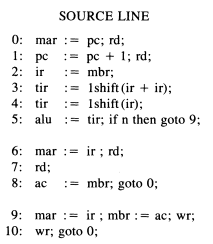
\includegraphics[width=6cm]{figures/ejemploTanenbaum}
 	\caption{Ejemplo de definición de microcódigo en simulador Tanenbaum.}
	\label{fig:tanenbaum_figure}
\end{figure}

En




\section{Simuladores para programación en ensamblador}
\label{sec:simuladores_ensamblador}
En esta sección, se explican los diferentes simuladores existentes para la programación en ensamblador. Los simuladores más conocidos para labores docentes, son SPIM, MARS y WebMIPS.

SPIM \cite{larus1990spim}, es un simulador de un procesador MIPS de 32 bits desarrollado a principios de 1990. En un primer momento implementaba el juego de instrucciones MIPS-1, utilizado por los computadores MIPS R2000/R3000. Actualmente, implementa la arquitectura MIPS32 más reciente y sus instrucciones adicionales. Permite ejecutar programas en ensamblador para esta arquitectura. Además, también permite depurar el código implementado, de forma que el alumno pueda corregir con mayor facilidad los errores cometidos. Este simulador, fue creado por James R. Larus y tiene versiones compiladas para Windows, Mac OS X y Unix/Linux e incluso tiene una versión básica para Android, aunque su diseño no está pensado para dispositivos móviles. Puesto que el simulador está totalmente enfocado al procesador MIPS, posee el juego completo de instrucciones para la versión de 32 bits del procesador y todas las directivas de las que consta el lenguaje. Otra característica que hace de SPIM un potente simulador, es proveer de un pequeño sistema operativo que soporta las principales llamadas al sistema mediante la instrucción syscall. SPIM, es un simulador que permite múltiples configuraciones mediante su interfaz de usuario, de manera que se puede indicar:

\begin{itemize}

\item Activación del uso de pseudoinstrucciones.

\item Simulación de predicción de saltos y accesos a memoria, con la latencia correspondiente.

\item Activación del uso del manejador de la señal trap y la carga del manejador personalizado.

\item Activación de la visualización de los mensajes en caso de ocurrir excepciones.

\item Activación del uso de "memory-mapped IO".

\end{itemize}

\begin{figure}[htbp]
 	\centering
 	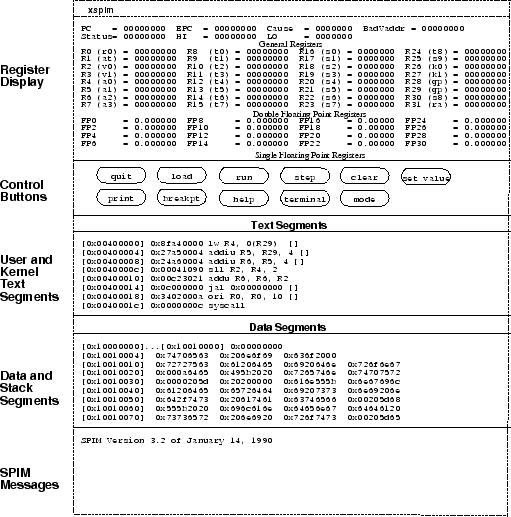
\includegraphics[width=8cm]{figures/spim_figure}
 	\caption{Interfaz SPIM.}
	\label{fig:spim_figure}
\end{figure}

SPIM, además cuenta con una versión más actualizada del simulador, que posee una interfaz gráfica más potente. Éste simulador se llama QtSPIM \cite{aguilar2013simuladores}, y cuenta con todas las características anteriormente mencionadas de SPIM.

\begin{figure}[htbp]
 	\centering
 	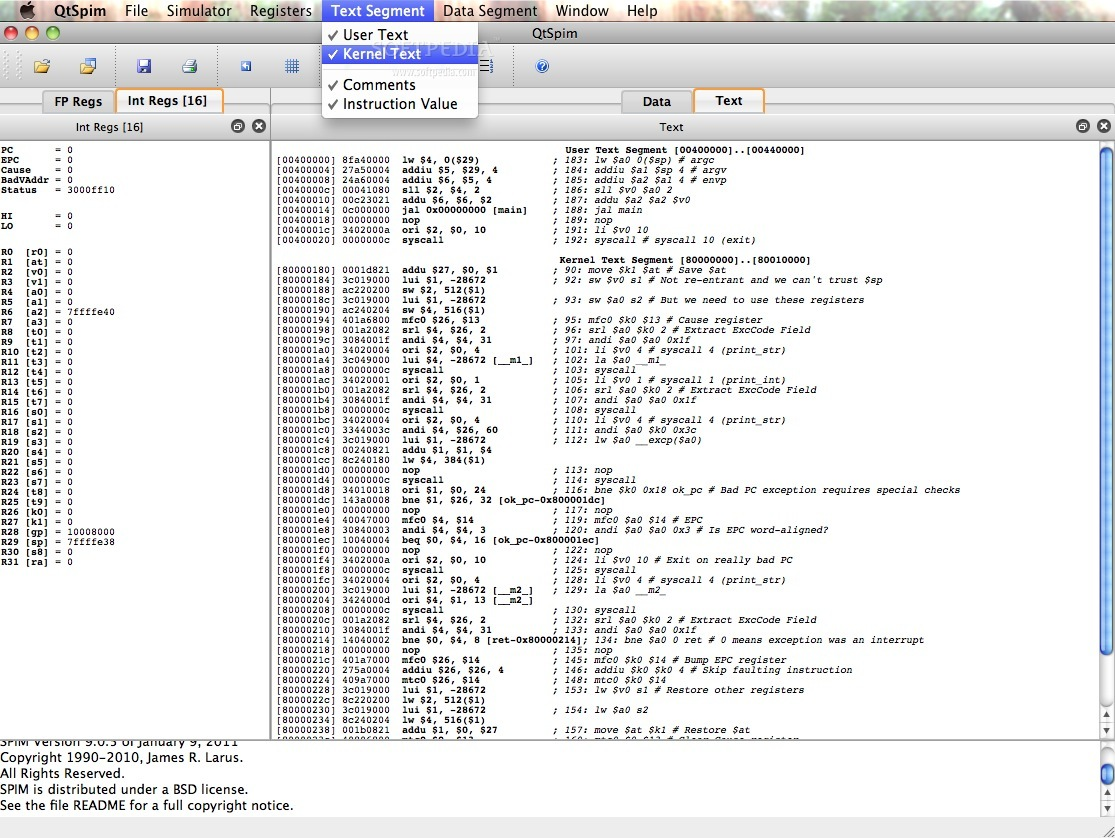
\includegraphics[width=12cm]{figures/qtspim_figure}
 	\caption{Interfaz QtSPIM.}
	\label{fig:qtspim_figure}
\end{figure}

MARS \cite{vollmar2006mars}, es un simulador con interfaz gráfica desarrollado en JAVA para el lenguaje ensamblador MIPS. Fue creado en el año 2005 como una alternativa del simulador SPIM y diseñado específicamente para las necesidades limitadas de cusos de pregrado. Está basado en la arquitectura MIPS RISC, que tiene un número pequeño de elementos del lenguaje e instrucciones. Consta de operaciones de entrada/salida, saltos, condiciones y operaciones aritmético-lógicas tanto enteras como en coma flotante. Alguna de las mejoras que incorpora MARS con respecto a SPIM son \cite{vegdahl2008mipspilot}: 

\begin{itemize}

\item Depuración más sencilla y cómoda, debido constar de GUI. Ésto se debe, a que para añadir un punto de ruptura, únicamente hay que clickar sobre un checkbox que tiene la instrucción.

\item Los programas puedes ejecutarse de forma inversa, lo que permite volver a un estado anterior de la máquina en la ejecución de un programa.

\item La velocidad de ejecución puede modificarse, de forma que si se ralentiza el usuario puede observar como cada instrucción se resalta cuando está siendo ejecutada y ver los cambios que se producen en los valores del banco de registros y de las ubicaciones de memoria.

\item  La memoria y los registros se pueden modificar de una manera WYSIWYG.

\item Incorpora un editor de texto, eliminando dependencias externas para el uso del simulador.

\item Permite que los desarrolladores puedan suministrar nuevos complementos, que por ejemplo, sirvan para extender la arquitectura o mostrar los datos de forma intuitiva.

\end{itemize}

\begin{figure}[htbp]
 	\centering
 	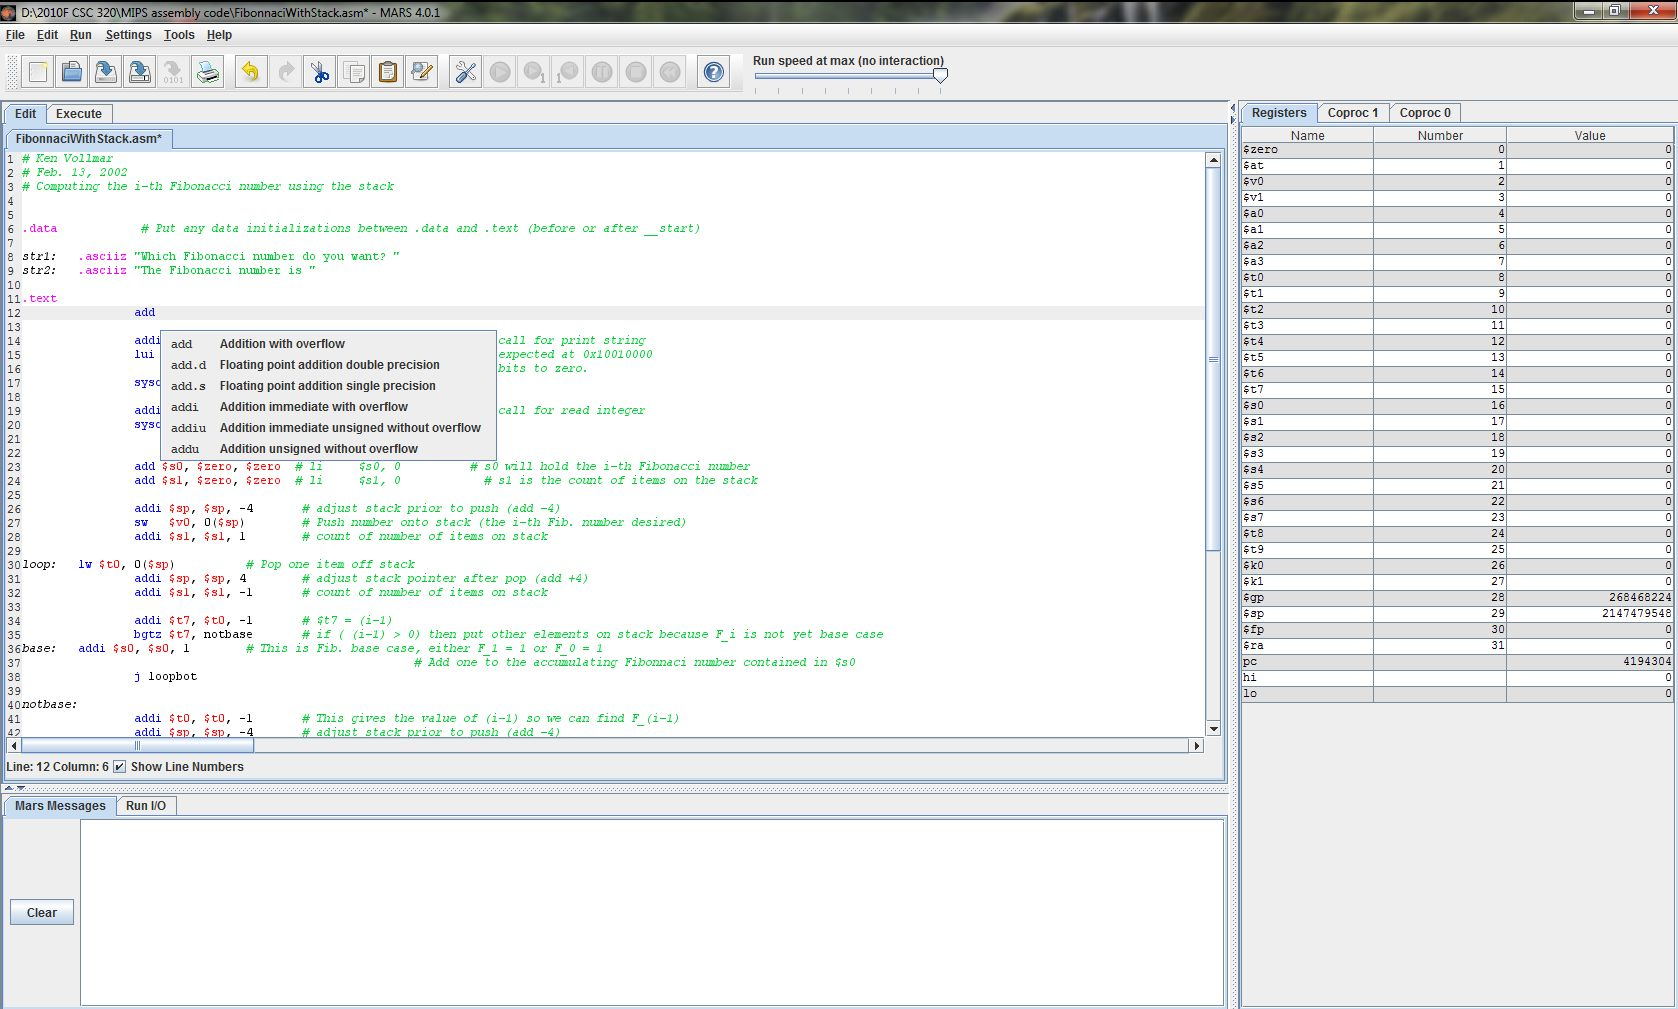
\includegraphics[width=12cm]{figures/mars_figure}
 	\caption{Interfaz MARS.}
	\label{fig:mars_figure}
\end{figure}

P88110, es emulador descrito en \cite{garcia2009p88110} que se basa en la emulación de un procesador superescalar. El propósito fundamental de este emulador, es mostrar el funcionamiento de este tipo de procesadores, haciendo visible el funcionamiento del pipeline y las dependencias existentes. Está basado en una arquitectura específica (MC88110) y pese a integrar el efecto de un procesador superescalar no integra la microprogramación, que haría de él un emulador completo.

\begin{figure}[htbp]
 	\centering
 	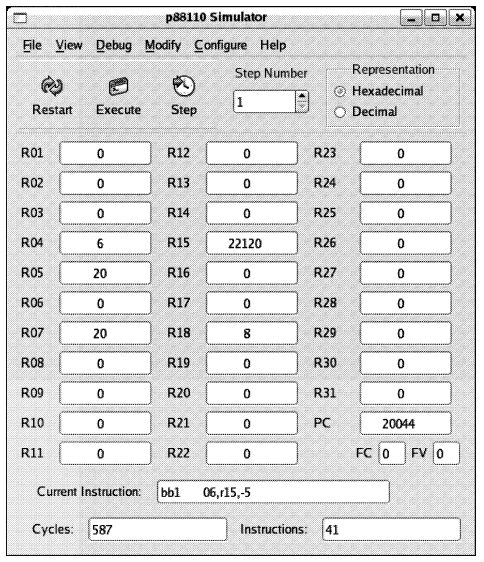
\includegraphics[width=12cm]{figures/em88110}
 	\caption{Interfaz em88110.}
	\label{fig:p88110_figure}
\end{figure}


WebMIPS \cite{branovic2004webmips}, es un simulador desarrollado en la Facultad de Ingeniería de la Información de Sienna, Italia. Está escrito en el lenguaje de programación ASP.NET y se utiliza mediante una página web, de forma que no requiere de su instalación en local. No soporta el juego completo de instrucciones de MIPS, sino que consta de un juego reducido de instrucciones que sirve de intruducción al estudio de arquitectura de computador. Con respecto a los anteriores simuladores mencionados, difiere al mostrar el esquema arquitectónico, indicando las 5 etapas de pipeline de las que consta el computador que simula. Otra característica, es la indicación del número de ciclos de reloj que consume la ejecución del programa. Tiene como objetivo principal la demostración de la ejecución del juego de instrucciones básico explicado durante la asignatura "Arquitectura de Computadores" impartida por los creadores del simulador.

Entre las diferentes características a destacar de este simulador, se encuentran:

\begin{itemize}
	
\item Verificación del código ensamblador, comprobando que no existen errores en la definición el código.

\item Dispone de códigos simples de ejemplo ("load-and-play") que facilitan la comprensión del funcionamiento del procesador.

\item Permite diferentes visualizaciones del estado de la memoria y los registros del procesador.

\item Consta de dos modos de ejecución: paso a paso y ejecución completa del programa.
	
\end{itemize}

\begin{figure}[htbp]
 	\centering
 	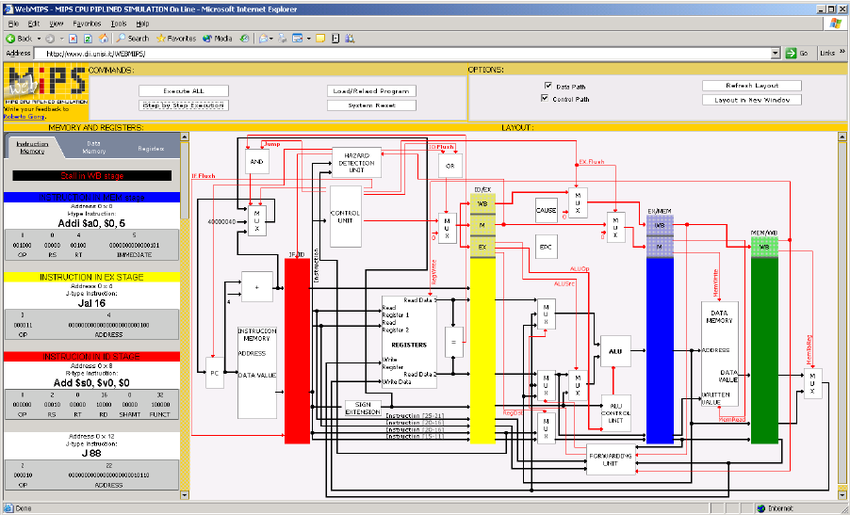
\includegraphics[width=12cm]{figures/webmips_figure}
 	\caption{ Interfaz WebMIPS.}
	\label{fig:webmips_figure}
\end{figure}

\clearpage

\section{Propuesta de simulación unificada}
\label{sec:propuesta_simulacion}
Hay distintas herramientas muy útiles para labores docentes relacionadas con la asignatura Estructura de Computadores, aunque como se comento previamente, no existe una herramienta que nos proporcione el desarrollo y simulación tanto a nivel de microcódigo como a nivel de ensamblador. WepSIM, une ambos aspectos ofreciendo:

\begin{itemize}
	\item Visión interrelacionada de la microprogramación y la programación en ensamblador.
	\item Flexibilidad en la plataforma usada, pensando el dispositivos móviles.
	\item Herramienta autocontenida, de forma que incorpora en sí misma tanto la ayuda como distintos ejemplos que favorecen la comprensión del simulador.
	\item Consta de un modelo hardware que puede ser modificado o ampliado en caso de ser necesario.
	\item Permite definir un amplio conjunto de instrucciones máquina.
	\item Puede ser usado como herramienta de microprogramación o de programación en ensamblador.
\end{itemize}

De este modo, con WepSIM se pretende crear un simulador unificado, abarcando los aspectos más relevantes de la asignatura "Estructura de Computadores" y permitiendo que todas las prácticas de la asignatura puedan realizarse en la misma plataforma, evitando la pérdida de tiempo y dificultad que supone para el alumno el habituarse a diferentes entornos para cada una de las prácticas.

WepSIM, se puede definir por tanto como un simulador de programación en ensamblador y microprogramación, flexible puesto que permite la personalización del juego de instrucciones de la máquina, multiplataforma puesto que permite su uso desde diferentes tipos de dispositivos, e interactivo al poder modificar la configuración de la máquina en tiempo de ejecución.

\begin{table}[htbp]
\ra{1.2}
\centering
%\resizebox{\textwidth}{%
\resizebox{\textwidth}{!}{
\begin{tabular}{@{}llllllll@{}}
\toprule
Simulador & SPIM & MARS & PC88110 & WebMIPS & WepSIM  & P8080E & MicMac\\ 
\midrule
Ensamblador				& \ding{51} & \ding{51} & \ding{51} & \ding{51} & \ding{51} &  &  \\
\midrule
Microprogramación				&  &  &  &  & \ding{51} & \ding{51} & \ding{51} \\
\midrule
Multiplataforma				& \ding{51} &  &  & \ding{51} & \ding{51} &  &  \\
\midrule
Interactivo				&  &  &  &  & \ding{51} &  &  \\
\midrule
Juego de instrucciones personalizable				&  &  &  &  & \ding{51} &  &  \\
\bottomrule
\end{tabular}
}
\caption{Comparación de simuladores de ensamblador y microcódigo.}
\label{tab:comparison_frameworks}
\end{table}


\lhead[\thepage]{CAPÍTULO \thechapter. ANÁLISIS}
\chead[]{}
\rhead[WepSIM: Simulador de procesador elemental con unidad de control microprogramada\leftmark]{\thepage}
\renewcommand{\headrulewidth}{0.5pt}

\lfoot[]{}
\cfoot[]{}
\rfoot[]{}
\renewcommand{\footrulewidth}{0pt}

%% This is an example first chapter.  You should put chapter/appendix that you
%% write into a separate file, and add a line \include{yourfilename} to
%% main.tex, where `yourfilename.tex' is the name of the chapter/appendix file.
%% You can process specific files by typing their names in at the 
%% \files=
%% prompt when you run the file main.tex through LaTeX.
\chapter{Análisis}
\label{ch:analysis}
\markboth{}{ANALYSIS}

El objetivo principal de este capitulo, es describir el proyecto mediante la obtención y especificación de los requisitos del simulador, que puede proporcionar información suficiente para un análisis detallado que, por lo tanto, puede servir para continuar diseñando e implementando (Capítulos \ref{ch:design}, \textit{\nameref{ch:design}}; and \ref{ch:implementation_and_deployment}, \textit{\nameref{ch:implementation_and_deployment}}) un software que cumpla con esos requisitos. 

Con el fin de obtener los requisitos del sistema, el tutor ha desempeñado el papel del cliente en diferentes reuniones, mientras que el alumno ha desempeñado los roles de analista, diseñador, programador y probador.

La sección \ref{sec:project_description} resume brevemente la descripción del proyecto. La sección \ref{sec:requirements} especifica los requisitos del sistema, empezando con los requisitos de usuario y finalizando con los requisitos funcionales y no-funcionales. Finalmente, la sección \ref{sec:regulatory_framework} indica el conjunto de leyes y regulaciones para la gestión del software.  

\section{Descripción del proyecto}
\label{sec:project_description}

El objetivo de este proyecto es construir una herramienta que permita simular con realismo el comportamiento de un procesador basado en la arquitectura indicada por el el tutor del proyecto, de forma que sirva como única herramienta para los alumnos a lo largo de la asignatura Estructura de Computadores.

\begin{figure}[htbp]
 	\centering
 	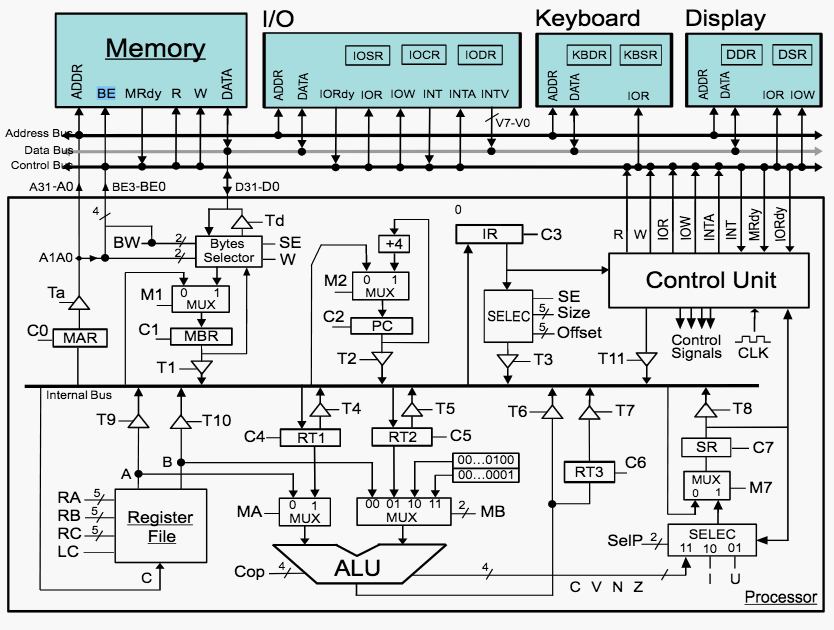
\includegraphics[width=12cm]{figures/cpu}
 	\caption{Arquitectura CPU WepSIM .}
	\label{fig:wepsimCPU_figure}
\end{figure}

\begin{figure}[htbp]
 	\centering
 	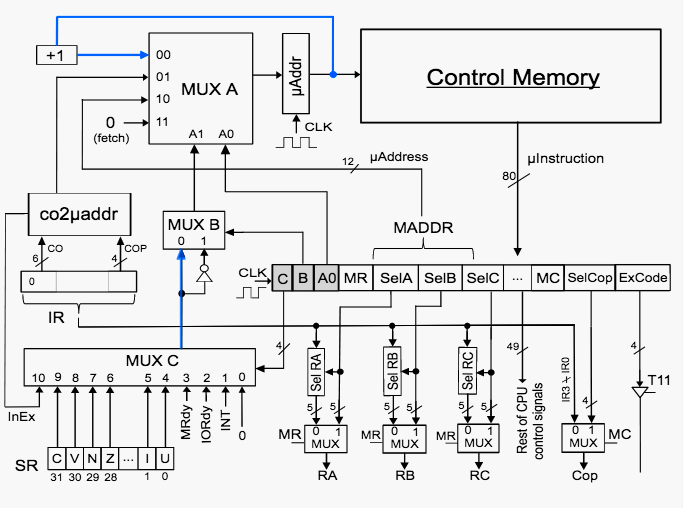
\includegraphics[width=12cm]{figures/controlUnit}
 	\caption{Arquitectura unidad de control WepSIM.}
	\label{fig:wepsimCU_figure}
\end{figure}

Los simuladores actuales para la enseñanza de Estructura de Computadores, están focalizados a una función concreta, como puede ser la simulación de cachés, la simulación de código ensamblador o la simulación de microcódigo entre otros, pero a la hora de unificar todas estas funcionalidades en una única herramienta, existe un vacío que genera una pérdida de tiempo en el aprendizaje de cada herramienta y la no posibilidad de ver una simulación completa.

El reto al que se enfrente cualquier simulador educativo es el de ser capaz de simular fielmente el funcionamiento de un dispositivo permitiendo al estudiante poder observar con el mayor detalle posible el comportamiento éste.

El sistema que se propone debe ser capaz de simular con realismo el comportamiento del procesador, permitiendo la definición del juego de instrucciones a utilizar para el posterior desarrollo de código ensamblador y su ejecución en el simulador con un alto nivel de detalle en cada uno de los ciclos de ejecución,.De esta forma, los estudiantes podrán comprender fácilmente los contenidos teóricos expuestos en la asignatura y serán capaces de realizar todas las prácticas en una misma herramienta, pudiendo ver de forma incremental el desarrollo de software de bajo nivel sobre un procesador elemental.

\section{Requisitos}
\label{sec:requirements}

Esta sección proporciona una descripción detallada de los requisitos de la aplicación. Para la tarea de la especificación de requisitos, se han seguido las prácticas recomendadas por IEEE \cite{ieee1998}. De acuerdo con estas prácticas, una buena especificación debe abordar la funcionalidad del software, los problemas de rendimiento, las interfaces externas, otras características no funcionales y las limitaciones de diseño o implementación.
Además, la especificación de los requisitos debe ser:

\begin{itemize}

\item \textbf{Completa:} el documento refleja todos los requisitos de software importantes.

\item \textbf{Consistente:} los requisitos no deben generar conflictos entre sí.

\item \textbf{Correcta:} cada requisito debe ser cumplido por el software según las necesidades del usuario.

% every requirement is one that the software shall meet according to the user needs.

\item \textbf{Modificable:} la estructura de la especificación permite cambios en los requisitos de una manera simple, completa y consistente.

\item \textbf{Clasificación basada en la importancia y la estabilidad:} cada requisito debe indicar su importancia y su estabilidad.

\item \textbf{Trazable:} el origen de cada requisito es claro y se puede hacer referencia fácilmente en otras etapas.

\item \textbf{Inequívoco:} cada requisito tiene una sola interpretación.

\item \textbf{Verificable:} Cada requisito debe ser verificable, es decir, existe algún proceso para verificar que el software cumple con cada requisito.

\end{itemize}

A partir de los requisitos de los usuarios, que constituyen una referencia informal al comportamiento del producto que el cliente espera, derivamos los requisitos de software (en este caso, requisitos funcionales y no funcionales) que guiaron el proceso de diseño con información específica sobre la funcionalidad del sistema y otras características. Los requisitos recuperados se estructuraron de acuerdo con el siguiente esquema:

%Starting from the user requirements, which constitute an informal reference to the product p%erformance that the client expects, we derived the software requirements (in this case, functional r%equirements and non-functional requirements) that guided the design process with specific %nformation on the functionality of the system and other characteristics. The retrieved requirements %were structured according with the following schema:

\begin{itemize}
\item[1.] \textbf{Requisitos de Usuario} 
	\begin{itemize}
		\item[(a)] \textbf{Capacidad:} el requisito describe la funcionalidad esperada del sistema como en casos de uso.
		\item[(b)] \textbf{Restricción:} el requisito especifica las restricciones o condiciones que el sistema debe cumplir.
	\end{itemize}	
\end{itemize}

\begin{itemize}
\item[2.] \textbf{Requisitos de Software}
	\begin{itemize}
	\item[(a)] 	\textbf{Funcionales}
		\begin{itemize}
		\item[i.] 	\textbf{Funcional:} el requisito describe la funcionalidad básica y el propósito del sistema mientras se minimiza la ambigüedad.
		\item[ii.] 	\textbf{Inverso:} el requisito limita la funcionalidad de la aplicación para aclarar su alcance.
		\end{itemize}

	\item[(b)] 	\textbf{No-Funcionales}
		\begin{itemize}
		\item[i.] 	\textbf{Rendimiento:} el requisito se relaciona con el rendimiento mínimo requerido del sistema resultante.
		\item[ii.] 	\textbf{Interfaz:} el requisito está relacionado con la interfaz de usuario de la aplicación.
		\item[iii.] 	\textbf{Escalabilidad:} el requisito está relacionado con la capacidad del sistema para adaptarse a cargas de trabajo cada vez mayores.
		\item[iv.] 	\textbf{Plataforma:} el requisito especifica las plataformas subyacentes de software y hardware en las que funcionará el sistema.
		\end{itemize}			
	\end{itemize}
\end{itemize}

La tabla \ref{tab:requirements_template} proporciona la plantilla utilizada para la especificación de requisitos. Tenga en cuenta que para los requisitos del usuario, el formato de identificación será UR-XYY, donde X indica el subtipo de requisito: requisitos de capacidad (C) o restricciones (R). YY corresponde al número de requisito en su subcategoría. Para los requisitos de software, se utilizará el formato de identificación SR-X-YZZ, donde X indica si es un requisito funcional (F) o no funcional (NF), e Y representa su subcategoría: funcional (F), inversa (I) ), Rendimiento (P), interfaz (UI), escalabilidad (S) o plataforma (PL). ZZ corresponde al número de requisito en su subcategoría.

\begin{center}
\begin{table*}[htbp]
\centering
\begin{tabular}{@{}p{2.5cm} p{9cm}@{}} 
\toprule
\textbf{ID} 				& Requisito ID. \\
\midrule
\textbf{Nombre} 			& Nombre del requisito. \\
\midrule
\textbf{Tipo} 			& Indica la categoría en la que se colocaría el requisito de acuerdo con el esquema descrito anteriormente. \\
\midrule
\textbf{Origen} 			& Constituye la fuente del requisito. Puede ser el usuario, otro requisito u otros actores involucrados en el proyecto. \\
\midrule
\textbf{Prioridad}		& Indica la prioridad del requisito según su importancia. Un requisito puede ser identificado como \textit{esencial}, \textit{condicional} or \textit{opcional}. \\
\midrule
\textbf{Estabilidad} 		& Indica la variabilidad del requisito a través del proceso de desarrollo, definido como \textit{estable} or \textit{inestable}. \\
\midrule
\textbf{Descripción} 	& Explicación detallada del requisito. \\
\bottomrule
\end{tabular}
\caption{Plantilla para la especificación de requisitos.}
\label{tab:requirements_template}
\end{table*}
\end{center}

\subsection{Requisitos de Usuario}

Esta subsección especifica los requisitos de usuario.

\begin{center}
\begin{table*}[htbp]
\centering
\begin{tabular}{@{}p{2.5cm} p{9cm}@{}} 
\toprule
\textbf{ID} 				& UR-C01 \\
\midrule
\textbf{Nombre} 			& Simulación del modelo hardware propuesto\\
\midrule
\textbf{Tipo} 			& Capacidad \\
\midrule
\textbf{Origen} 			& Usuario \\
\midrule
\textbf{Prioridad}		& Esencial \\
\midrule
\textbf{Estabilidad} 		& Estable \\
\midrule
\textbf{Descripción} 	& La herramienta simulará el comportamiento de la arquitectura definida para la asignatura Estructura de Computadores. \\
\bottomrule
\end{tabular}
\caption{Requisito de usuario UR-C01.}
\label{tab:urc01}
\end{table*}
\end{center}

\begin{center}
\begin{table*}[htbp]
\centering
\begin{tabular}{@{}p{2.5cm} p{9cm}@{}} 
\toprule
\textbf{ID} 				& UR-C02 \\
\midrule
\textbf{Nombre} 			& Definición de juego de instrucciones del simulador \\
\midrule
\textbf{Tipo} 			& Capacidad \\
\midrule
\textbf{Origen} 			& Usuario \\
\midrule
\textbf{Prioridad}		& Esencial \\
\midrule
\textbf{Estabilidad} 		& Estable \\
\midrule
\textbf{Descripción} 	& La herramienta debe permitir la definición del juego de instrucciones a utilizar por el usuario siguiendo el formato especificado por el tutor. \\
\bottomrule
\end{tabular}
\caption{Requisito de usuario UR-C02.}
\label{tab:urc02}
\end{table*}
\end{center}

\begin{center}
\begin{table*}[htbp]
\centering
\begin{tabular}{@{}p{2.5cm} p{9cm}@{}} 
\toprule
\textbf{ID} 				& UR-C03 \\
\midrule
\textbf{Nombre} 			& Operaciones con el juego de instrucciones \\
\midrule
\textbf{Tipo} 			& Capacidad \\
\midrule
\textbf{Origen} 			& Usuario \\
\midrule
\textbf{Prioridad}		& Esencial \\
\midrule
\textbf{Estabilidad} 		& Estable \\
\midrule
\textbf{Descripción} 	& La herramienta debe permitir al usuario las siguientes operaciones con el juego de instrucciones: cargar desde fichero, exportar a un fichero y generar el firmware. \\
\bottomrule
\end{tabular}
\caption{Requisito de usuario UR-C03.}
\label{tab:urc03}
\end{table*}
\end{center}

\begin{center}
\begin{table*}[htbp]
\centering
\begin{tabular}{@{}p{2.5cm} p{9cm}@{}} 
\toprule
\textbf{ID} 				& UR-C04 \\
\midrule
\textbf{Nombre} 			& Definición de juego del código ensamblador \\
\midrule
\textbf{Tipo} 			& Capacidad \\
\midrule
\textbf{Origen} 			& Usuario \\
\midrule
\textbf{Prioridad}		& Esencial \\
\midrule
\textbf{Estabilidad} 		& Estable \\
\midrule
\textbf{Descripción} 	& La herramienta debe permitir la definición del código ensamblador a simular siguiendo el formato utilizado en la asignatura Estructura de Computadores y el juego de instrucciones cargado previamente. \\
\bottomrule
\end{tabular}
\caption{Requisito de usuario UR-C04.}
\label{tab:urc04}
\end{table*}
\end{center}

\begin{center}
\begin{table*}[htbp]
\centering
\begin{tabular}{@{}p{2.5cm} p{9cm}@{}} 
\toprule
\textbf{ID} 				& UR-C05 \\
\midrule
\textbf{Nombre} 			& Operaciones con el código ensamblador \\
\midrule
\textbf{Tipo} 			& Capacidad \\
\midrule
\textbf{Origen} 			& Usuario \\
\midrule
\textbf{Prioridad}		& Esencial \\
\midrule
\textbf{Estabilidad} 		& Estable \\
\midrule
\textbf{Descripción} 	& La herramienta debe permitir al usuario las siguientes operaciones con el código ensamblador: cargar desde fichero, exportar a un fichero y generar el binario asociado. \\
\bottomrule
\end{tabular}
\caption{Requisito de usuario UR-C05.}
\label{tab:urc05}
\end{table*}
\end{center}

\begin{center}
\begin{table*}[htbp]
\centering
\begin{tabular}{@{}p{2.5cm} p{9cm}@{}} 
\toprule
\textbf{ID} 				& UR-C06 \\
\midrule
\textbf{Nombre} 			& Tipos de simulación \\
\midrule
\textbf{Tipo} 			& Capacidad \\
\midrule
\textbf{Origen} 			& Usuario \\
\midrule
\textbf{Prioridad}		& Esencial \\
\midrule
\textbf{Estabilidad} 		& Estable \\
\midrule
\textbf{Descripción} 	& La herramienta debe permitir tres tipos diferentes de simulación: simulación ciclo a ciclo de reloj, simulación instrucción a instrucción y simulación completa del código.\\
\bottomrule
\end{tabular}
\caption{Requisito de usuario UR-C06.}
\label{tab:urc06}
\end{table*}
\end{center}

\begin{center}
\begin{table*}[htbp]
\centering
\begin{tabular}{@{}p{2.5cm} p{9cm}@{}} 
\toprule
\textbf{ID} 				& UR-C07 \\
\midrule
\textbf{Nombre} 			& Configuración de la velocidad de las simulaciones \\
\midrule
\textbf{Tipo} 			& Capacidad \\
\midrule
\textbf{Origen} 			& Usuario \\
\midrule
\textbf{Prioridad}		& Esencial \\
\midrule
\textbf{Estabilidad} 		& Estable \\
\midrule
\textbf{Descripción} 	& La herramienta debe permitir al usuario seleccionar la velocidad de la simulación. \\
\bottomrule
\end{tabular}
\caption{Requisito de usuario UR-C07.}
\label{tab:urc07}
\end{table*}
\end{center}

\begin{center}
\begin{table*}[htbp]
\centering
\begin{tabular}{@{}p{2.5cm} p{9cm}@{}} 
\toprule
\textbf{ID} 				& UR-C08 \\
\midrule
\textbf{Nombre} 			& Esquemas de la arquitectura \\
\midrule
\textbf{Tipo} 			& Capacidad \\
\midrule
\textbf{Origen} 			& Usuario \\
\midrule
\textbf{Prioridad}		& Esencial \\
\midrule
\textbf{Estabilidad} 		& Estable \\
\midrule
\textbf{Descripción} 	& La herramienta debe mostrar la arquitectura de la CPU y la Unidad de Control que forman el simulador. \\
\bottomrule
\end{tabular}
\caption{Requisito de usuario UR-C08.}
\label{tab:urc08}
\end{table*}
\end{center}

\begin{center}
\begin{table*}[htbp]
\centering
\begin{tabular}{@{}p{2.5cm} p{9cm}@{}} 
\toprule
\textbf{ID} 				& UR-C09 \\
\midrule
\textbf{Nombre} 			& Información a mostrar \\
\midrule
\textbf{Tipo} 			& Capacidad \\
\midrule
\textbf{Origen} 			& Usuario \\
\midrule
\textbf{Prioridad}		& Esencial \\
\midrule
\textbf{Estabilidad} 		& Estable \\
\midrule
\textbf{Descripción} 	& La herramienta debe mostrar al usuario la información del estado del simulador en cada paso de la simulación. \\
\bottomrule
\end{tabular}
\caption{Requisito de usuario UR-C09.}
\label{tab:urc09}
\end{table*}
\end{center}


\begin{center}
\begin{table*}[htbp]
\centering
\begin{tabular}{@{}p{2.5cm} p{9cm}@{}} 
\toprule
\textbf{ID} 				& UR-R01 \\
\midrule
\textbf{Nombre} 			& Herramienta web\\
\midrule
\textbf{Tipo} 			& Restricción \\
\midrule
\textbf{Origen} 			& Usuario \\
\midrule
\textbf{Prioridad}		& Esencial \\
\midrule
\textbf{Estabilidad} 		& Estable \\
\midrule
\textbf{Descripción} 	& El simulador debe de ser una herramienta web. \\
\bottomrule
\end{tabular}
\caption{Requisito de usuario UR-R01.}
\label{tab:urr01}
\end{table*}
\end{center}

\begin{center}
\begin{table*}[htbp]
\centering
\begin{tabular}{@{}p{2.5cm} p{9cm}@{}} 
\toprule
\textbf{ID} 				& UR-R02 \\
\midrule
\textbf{Nombre} 			& Navegadores web \\
\midrule
\textbf{Tipo} 			& Restricción \\
\midrule
\textbf{Origen} 			& Usuario \\
\midrule
\textbf{Prioridad}		& Esencial \\
\midrule
\textbf{Estabilidad} 		& Estable \\
\midrule
\textbf{Descripción} 	& El simulador debe de funcionar en los siguiente navegadores web: Microsoft edge, Mozilla Firefox, Google Chrome y Safari. \\
\bottomrule
\end{tabular}
\caption{Requisito de usuario UR-R02.}
\label{tab:urr02}
\end{table*}
\end{center}

\begin{center}
\begin{table*}[htbp]
\centering
\begin{tabular}{@{}p{2.5cm} p{9cm}@{}} 
\toprule
\textbf{ID} 				& UR-R03 \\
\midrule
\textbf{Nombre} 			& Interfaz de usuario \\
\midrule
\textbf{Tipo} 			& Restricción \\
\midrule
\textbf{Origen} 			& Usuario \\
\midrule
\textbf{Prioridad}		& Esencial \\
\midrule
\textbf{Estabilidad} 		& Estable \\
\midrule
\textbf{Descripción} 	& La interfaz de usuario debe de ser compatible para uso en pc's y smartphones. \\
\bottomrule
\end{tabular}
\caption{Requisito de usuario UR-R03.}
\label{tab:urr03}
\end{table*}
\end{center}

\begin{center}
\begin{table*}[htbp]
\centering
\begin{tabular}{@{}p{2.5cm} p{9cm}@{}} 
\toprule
\textbf{ID} 				& UR-R04 \\
\midrule
\textbf{Nombre} 			& Tiempo por ciclo de reloj \\
\midrule
\textbf{Tipo} 			& Restricción \\
\midrule
\textbf{Origen} 			& Usuario \\
\midrule
\textbf{Prioridad}		& Esencial \\
\midrule
\textbf{Estabilidad} 		& Estable \\
\midrule
\textbf{Descripción} 	& El tiempo de ejecución de un ciclo de reloj del simulador no debe de sobrepasar 0,1 segundos. \\
\bottomrule
\end{tabular}
\caption{Requisito de usuario UR-R04.}
\label{tab:urr04}
\end{table*}
\end{center}

\begin{center}
\begin{table*}[htbp]
\centering
\begin{tabular}{@{}p{2.5cm} p{9cm}@{}} 
\toprule
\textbf{ID} 				& UR-R05 \\
\midrule
\textbf{Nombre} 			& Ejecución en local \\
\midrule
\textbf{Tipo} 			& Restricción \\
\midrule
\textbf{Origen} 			& Usuario \\
\midrule
\textbf{Prioridad}		& Esencial \\
\midrule
\textbf{Estabilidad} 		& Estable \\
\midrule
\textbf{Descripción} 	& Las simulaciones serán realizadas en la máquina del usuario, siendo únicamente necesario el servidor para el acceso a la herramienta. \\
\bottomrule
\end{tabular}
\caption{Requisito de usuario UR-R05.}
\label{tab:urr05}
\end{table*}
\end{center}

\begin{center}
\begin{table*}[htbp]
\centering
\begin{tabular}{@{}p{2.5cm} p{9cm}@{}} 
\toprule
\textbf{ID} 				& UR-R06 \\
\midrule
\textbf{Nombre} 			& Conexión a internet \\
\midrule
\textbf{Tipo} 			& Restricción \\
\midrule
\textbf{Origen} 			& Usuario \\
\midrule
\textbf{Prioridad}		& Esencial \\
\midrule
\textbf{Estabilidad} 		& Estable \\
\midrule
\textbf{Descripción} 	& Para realizar una simulación, el dispositivo del usuario no necesita conexión a internet. \\
\bottomrule
\end{tabular}
\caption{Requisito de usuario UR-R06.}
\label{tab:urr06}
\end{table*}
\end{center}

\begin{center}
\begin{table*}[htbp]
\centering
\begin{tabular}{@{}p{2.5cm} p{9cm}@{}} 
\toprule
\textbf{ID} 				& UR-R07 \\
\midrule
\textbf{Nombre} 			& Tecnologías de desarrollo \\
\midrule
\textbf{Tipo} 			& Restricción \\
\midrule
\textbf{Origen} 			& Usuario \\
\midrule
\textbf{Prioridad}		& Esencial \\
\midrule
\textbf{Estabilidad} 		& Estable \\
\midrule
\textbf{Descripción} 	& El simulador debe de ser desarrollado mediante el lenguaje de programación JavaScript, posibilitando migraciones futuras. \\
\bottomrule
\end{tabular}
\caption{Requisito de usuario UR-R07.}
\label{tab:urr07}
\end{table*}
\end{center}


\iffalse

\begin{center}
\begin{table*}[htbp]
\centering
\begin{tabular}{@{}p{2.5cm} p{9cm}@{}} 
\toprule
\textbf{ID} 				& UR-C00 \\
\midrule
\textbf{Nombre} 			& a \\
\midrule
\textbf{Tipo} 			& a \\
\midrule
\textbf{Origen} 			& a \\
\midrule
\textbf{Prioridad}		& a \\
\midrule
\textbf{Estabilidad} 		& a \\
\midrule
\textbf{Descripción} 	& a \\
\bottomrule
\end{tabular}
\caption{Requisito de usuario UR-C00.}
\label{tab:urc00}
\end{table*}
\end{center}

\fi

\clearpage
\subsection{Requisitos Funcionales}

Esta subsección especifica los requisitos funcionales.

\begin{center}
\begin{table*}[htbp]
\centering
\begin{tabular}{@{}p{2.5cm} p{9cm}@{}} 
\toprule
\textbf{ID} 				& SR-F-F01 \\
\midrule
\textbf{Nombre} 			& Arquitectura de 32 bits \\
\midrule
\textbf{Tipo} 			& Funcional \\
\midrule
\textbf{Origen} 			& UR-C01 \\
\midrule
\textbf{Prioridad}		& Esencial \\
\midrule
\textbf{Estabilidad} 		& Estable \\
\midrule
\textbf{Descripción} 	& La herramienta debe simular una arquitectura de 32 bits. \\
\bottomrule
\end{tabular}
\caption{Requisito Funcional SR-F-F01.}
\label{tab:srff01}
\end{table*}
\end{center}

\begin{center}
\begin{table*}[htbp]
\centering
\begin{tabular}{@{}p{2.5cm} p{9cm}@{}} 
\toprule
\textbf{ID} 				& SR-F-F02 \\
\midrule
\textbf{Nombre} 			& Unidad de control microprogramable \\
\midrule
\textbf{Tipo} 			& Funcional \\
\midrule
\textbf{Origen} 			& UR-C01 \\
\midrule
\textbf{Prioridad}		& Esencial \\
\midrule
\textbf{Estabilidad} 		& Estable \\
\midrule
\textbf{Descripción} 	& La unidad de control debe de ser micoprogramable. \\
\bottomrule
\end{tabular}
\caption{Requisito Funcional SR-F-F02.}
\label{tab:srff02}
\end{table*}
\end{center}

\begin{center}
\begin{table*}[htbp]
\centering
\begin{tabular}{@{}p{2.5cm} p{9cm}@{}} 
\toprule
\textbf{ID} 				& SR-F-F03 \\
\midrule
\textbf{Nombre} 			& Datos en complemento a2 \\
\midrule
\textbf{Tipo} 			& Funcional \\
\midrule
\textbf{Origen} 			& UR-C01 \\
\midrule
\textbf{Prioridad}		& Esencial \\
\midrule
\textbf{Estabilidad} 		& Estable \\
\midrule
\textbf{Descripción} 	& La herramienta operará con números enteros en complemento a2. \\
\bottomrule
\end{tabular}
\caption{Requisito Funcional SR-F-F03.}
\label{tab:srff03}
\end{table*}
\end{center}

\begin{center}
\begin{table*}[htbp]
\centering
\begin{tabular}{@{}p{2.5cm} p{9cm}@{}} 
\toprule
\textbf{ID} 				& SR-F-F04 \\
\midrule
\textbf{Nombre} 			& Definición de juego de instrucciones \\
\midrule
\textbf{Tipo} 			& Funcional \\
\midrule
\textbf{Origen} 			& UR-C02 \\
\midrule
\textbf{Prioridad}		& Esencial \\
\midrule
\textbf{Estabilidad} 		& Estable \\
\midrule
\textbf{Descripción} 	& La herramienta debe permitir al usuario la definición del juego de instrucciones a utilizar.\\
\bottomrule
\end{tabular}
\caption{Requisito Funcional SR-F-F04.}
\label{tab:srff04}
\end{table*}
\end{center}

\begin{center}
\begin{table*}[htbp]
\centering
\begin{tabular}{@{}p{2.5cm} p{9cm}@{}} 
\toprule
\textbf{ID} 				& SR-F-F05 \\
\midrule
\textbf{Nombre} 			& Formato del juego de instrucciones\\
\midrule
\textbf{Tipo} 			& Funcional \\
\midrule
\textbf{Origen} 			& UR-C02 \\
\midrule
\textbf{Prioridad}		& Esencial \\
\midrule
\textbf{Estabilidad} 		& Estable \\
\midrule
\textbf{Descripción} 	& El juego de instrucciones debe seguir el formato utilizado en la asignatura Estructura de Computadores, definiendo instrucciones del lenguaje ensamblador, nombrado de los registros y pseudoinstrucciones. \\
\bottomrule
\end{tabular}
\caption{Requisito Funcional SR-F-F05.}
\label{tab:srff05}
\end{table*}
\end{center}

\begin{center}
\begin{table*}[htbp]
\centering
\begin{tabular}{@{}p{2.5cm} p{9cm}@{}} 
\toprule
\textbf{ID} 				& SR-F-F06 \\
\midrule
\textbf{Nombre} 			& Modificación del juego de instrucciones\\
\midrule
\textbf{Tipo} 			& Funcional \\
\midrule
\textbf{Origen} 			& UR-C03 \\
\midrule
\textbf{Prioridad}		& Esencial \\
\midrule
\textbf{Estabilidad} 		& Estable \\
\midrule
\textbf{Descripción} 	& La herramienta debe de permitir la modificación del juego de instrucciones a utilizar por el usuario. \\
\bottomrule
\end{tabular}
\caption{Requisito Funcional SR-F-F06.}
\label{tab:srff06}
\end{table*}
\end{center}

\begin{center}
\begin{table*}[htbp]
\centering
\begin{tabular}{@{}p{2.5cm} p{9cm}@{}} 
\toprule
\textbf{ID} 				& SR-F-F07 \\
\midrule
\textbf{Nombre} 			& Carga de juego de instrucciones\\
\midrule
\textbf{Tipo} 			& Funcional \\
\midrule
\textbf{Origen} 			& UR-C03 \\
\midrule
\textbf{Prioridad}		& Esencial \\
\midrule
\textbf{Estabilidad} 		& Estable \\
\midrule
\textbf{Descripción} 	& La herramienta debe permitir la carga de un fichero que contenga el juego de instrucciones. \\
\bottomrule
\end{tabular}
\caption{Requisito Funcional SR-F-F07.}
\label{tab:srff07}
\end{table*}
\end{center}

\begin{center}
\begin{table*}[htbp]
\centering
\begin{tabular}{@{}p{2.5cm} p{9cm}@{}} 
\toprule
\textbf{ID} 				& SR-F-F08 \\
\midrule
\textbf{Nombre} 			& Exportar juego de instrucciones\\
\midrule
\textbf{Tipo} 			& Funcional \\
\midrule
\textbf{Origen} 			& UR-C03 \\
\midrule
\textbf{Prioridad}		& Esencial \\
\midrule
\textbf{Estabilidad} 		& Estable \\
\midrule
\textbf{Descripción} 	& La herramienta debe permitir exportar el juego de instrucciones en un fichero. \\
\bottomrule
\end{tabular}
\caption{Requisito Funcional SR-F-F08.}
\label{tab:srff08}
\end{table*}
\end{center}

\begin{center}
\begin{table*}[htbp]
\centering
\begin{tabular}{@{}p{2.5cm} p{9cm}@{}} 
\toprule
\textbf{ID} 				& SR-F-F09 \\
\midrule
\textbf{Nombre} 			& Generación firmware del simulador\\
\midrule
\textbf{Tipo} 			& Funcional \\
\midrule
\textbf{Origen} 			& UR-C03 \\
\midrule
\textbf{Prioridad}		& Esencial \\
\midrule
\textbf{Estabilidad} 		& Estable \\
\midrule
\textbf{Descripción} 	& La herramienta debe de generar el firmware simulador a partir del juego de instrucciones definido y cargado por el usuario. \\
\bottomrule
\end{tabular}
\caption{Requisito Funcional SR-F-F09.}
\label{tab:srff09}
\end{table*}
\end{center}

\begin{center}
\begin{table*}[htbp]
\centering
\begin{tabular}{@{}p{2.5cm} p{9cm}@{}} 
\toprule
\textbf{ID} 				& SR-F-F10 \\
\midrule
\textbf{Nombre} 			& Definición del código ensamblador\\
\midrule
\textbf{Tipo} 			& Funcional \\
\midrule
\textbf{Origen} 			& UR-C04 \\
\midrule
\textbf{Prioridad}		& Esencial \\
\midrule
\textbf{Estabilidad} 		& Estable \\
\midrule
\textbf{Descripción} 	& La herramienta debe permitir al usuario la definición del código ensamblador a utilizar en la simulación. \\
\bottomrule
\end{tabular}
\caption{Requisito Funcional SR-F-F10.}
\label{tab:srff10}
\end{table*}
\end{center}

\begin{center}
\begin{table*}[htbp]
\centering
\begin{tabular}{@{}p{2.5cm} p{9cm}@{}} 
\toprule
\textbf{ID} 				& SR-F-F11 \\
\midrule
\textbf{Nombre} 			& Formato del código ensamblador\\
\midrule
\textbf{Tipo} 			& Funcional \\
\midrule
\textbf{Origen} 			& UR-C04 \\
\midrule
\textbf{Prioridad}		& Esencial \\
\midrule
\textbf{Estabilidad} 		& Estable \\
\midrule
\textbf{Descripción} 	& El código ensamblador a simular debe de seguir el formato utilizado en la asignatura Estructura de Computadores, utilizando el lenguaje definido en el juego de instrucciones.\\
\bottomrule
\end{tabular}
\caption{Requisito Funcional SR-F-F11.}
\label{tab:srff11}
\end{table*}
\end{center}

\begin{center}
\begin{table*}[htbp]
\centering
\begin{tabular}{@{}p{2.5cm} p{9cm}@{}} 
\toprule
\textbf{ID} 				& SR-F-F12 \\
\midrule
\textbf{Nombre} 			& Edición del código ensamblador\\
\midrule
\textbf{Tipo} 			& Funcional \\
\midrule
\textbf{Origen} 			& UR-C05 \\
\midrule
\textbf{Prioridad}		& Esencial \\
\midrule
\textbf{Estabilidad} 		& Estable \\
\midrule
\textbf{Descripción} 	& La heramienta debe permitir modificar el código ensamblador. \\
\bottomrule
\end{tabular}
\caption{Requisito Funcional SR-F-F12.}
\label{tab:srff12}
\end{table*}
\end{center}

\begin{center}
\begin{table*}[htbp]
\centering
\begin{tabular}{@{}p{2.5cm} p{9cm}@{}} 
\toprule
\textbf{ID} 				& SR-F-F13 \\
\midrule
\textbf{Nombre} 			& Carga del código ensamblador\\
\midrule
\textbf{Tipo} 			& Funcional \\
\midrule
\textbf{Origen} 			& UR-C05 \\
\midrule
\textbf{Prioridad}		& Esencial \\
\midrule
\textbf{Estabilidad} 		& Estable \\
\midrule
\textbf{Descripción} 	& La herramienta debe permitir la carga de un fichero que contenga el código ensamblador. \\
\bottomrule
\end{tabular}
\caption{Requisito Funcional SR-F-F13.}
\label{tab:srff13}
\end{table*}
\end{center}

\begin{center}
\begin{table*}[htbp]
\centering
\begin{tabular}{@{}p{2.5cm} p{9cm}@{}} 
\toprule
\textbf{ID} 				& SR-F-F14 \\
\midrule
\textbf{Nombre} 			& Generación ejecutable del codigo ensamblador\\
\midrule
\textbf{Tipo} 			& Funcional \\
\midrule
\textbf{Origen} 			& UR-C05 \\
\midrule
\textbf{Prioridad}		& Esencial \\
\midrule
\textbf{Estabilidad} 		& Estable \\
\midrule
\textbf{Descripción} 	& La herramienta debe de generar el binario ejecutable asociado al código ensamblador definido para la simulación. \\
\bottomrule
\end{tabular}
\caption{Requisito Funcional SR-F-F14.}
\label{tab:srff14}
\end{table*}
\end{center}

\begin{center}
\begin{table*}[htbp]
\centering
\begin{tabular}{@{}p{2.5cm} p{9cm}@{}} 
\toprule
\textbf{ID} 				& SR-F-F15 \\
\midrule
\textbf{Nombre} 			& Simulación ciclo a ciclo de reloj\\
\midrule
\textbf{Tipo} 			& Funcional \\
\midrule
\textbf{Origen} 			& UR-C06 \\
\midrule
\textbf{Prioridad}		& Esencial \\
\midrule
\textbf{Estabilidad} 		& Estable \\
\midrule
\textbf{Descripción} 	& La herramienta debe de permitir la simulación ciclo a ciclo de reloj del código ensamblador cargado por el usuario. \\
\bottomrule
\end{tabular}
\caption{Requisito Funcional SR-F-F15.}
\label{tab:srff15}
\end{table*}
\end{center}

\begin{center}
\begin{table*}[htbp]
\centering
\begin{tabular}{@{}p{2.5cm} p{9cm}@{}} 
\toprule
\textbf{ID} 				& SR-F-F16 \\
\midrule
\textbf{Nombre} 			& Simulación instrucción a instrucción\\
\midrule
\textbf{Tipo} 			& Funcional \\
\midrule
\textbf{Origen} 			& UR-C06 \\
\midrule
\textbf{Prioridad}		& Esencial \\
\midrule
\textbf{Estabilidad} 		& Estable \\
\midrule
\textbf{Descripción} 	& La herramienta debe de permitir la simulación instrucción a instrucción del código ensamblador cargado por el usuario. \\
\bottomrule
\end{tabular}
\caption{Requisito Funcional SR-F-F16.}
\label{tab:srff16}
\end{table*}
\end{center}

\begin{center}
\begin{table*}[htbp]
\centering
\begin{tabular}{@{}p{2.5cm} p{9cm}@{}} 
\toprule
\textbf{ID} 				& SR-F-F17 \\
\midrule
\textbf{Nombre} 			& Simulación completa\\
\midrule
\textbf{Tipo} 			& Funcional \\
\midrule
\textbf{Origen} 			& UR-C06 \\
\midrule
\textbf{Prioridad}		& Esencial \\
\midrule
\textbf{Estabilidad} 		& Estable \\
\midrule
\textbf{Descripción} 	& La herramienta debe de permitir la simulación completa del código ensamblador cargado por el usuario. \\
\bottomrule
\end{tabular}
\caption{Requisito Funcional SR-F-F17.}
\label{tab:srff17}
\end{table*}
\end{center}

\begin{center}
\begin{table*}[htbp]
\centering
\begin{tabular}{@{}p{2.5cm} p{9cm}@{}} 
\toprule
\textbf{ID} 				& SR-F-F18 \\
\midrule
\textbf{Nombre} 			& Velocidad de simulación\\
\midrule
\textbf{Tipo} 			& Funcional \\
\midrule
\textbf{Origen} 			& UR-C07 \\
\midrule
\textbf{Prioridad}		& Esencial \\
\midrule
\textbf{Estabilidad} 		& Estable \\
\midrule
\textbf{Descripción} 	& La herramienta debe de permitir al usuario elegir la velocidad de simulación del código ensamblador cargado. \\
\bottomrule
\end{tabular}
\caption{Requisito Funcional SR-F-F18.}
\label{tab:srff18}
\end{table*}
\end{center}

\begin{center}
\begin{table*}[htbp]
\centering
\begin{tabular}{@{}p{2.5cm} p{9cm}@{}} 
\toprule
\textbf{ID} 				& SR-F-F19 \\
\midrule
\textbf{Nombre} 			& Esquema CPU\\
\midrule
\textbf{Tipo} 			& Funcional \\
\midrule
\textbf{Origen} 			& UR-C08 \\
\midrule
\textbf{Prioridad}		& Esencial \\
\midrule
\textbf{Estabilidad} 		& Estable \\
\midrule
\textbf{Descripción} 	& La herramienta debe de mostrar el esquema de la CPU del simulador, modificando el color de las señales activas y buses de datos actualizados en cada ciclo de reloj. \\
\bottomrule
\end{tabular}
\caption{Requisito Funcional SR-F-F19.}
\label{tab:srff19}
\end{table*}
\end{center}

\begin{center}
\begin{table*}[htbp]
\centering
\begin{tabular}{@{}p{2.5cm} p{9cm}@{}} 
\toprule
\textbf{ID} 				& SR-F-F20 \\
\midrule
\textbf{Nombre} 			& Esquema Unidad de Control\\
\midrule
\textbf{Tipo} 			& Funcional \\
\midrule
\textbf{Origen} 			& UR-C08 \\
\midrule
\textbf{Prioridad}		& Esencial \\
\midrule
\textbf{Estabilidad} 		& Estable \\
\midrule
\textbf{Descripción} 	& La herramienta debe de mostrar el esquema de la Unidad de Control del simulador, modificando el color de las señales activas y buses de datos actualizados en cada ciclo de reloj. \\
\bottomrule
\end{tabular}
\caption{Requisito Funcional SR-F-F20.}
\label{tab:srff20}
\end{table*}
\end{center}

\begin{center}
\begin{table*}[htbp]
\centering
\begin{tabular}{@{}p{2.5cm} p{9cm}@{}} 
\toprule
\textbf{ID} 				& SR-F-F21\\
\midrule
\textbf{Nombre} 			& Información de la simulación\\
\midrule
\textbf{Tipo} 			& Funcional \\
\midrule
\textbf{Origen} 			& UR-C09 \\
\midrule
\textbf{Prioridad}		& Esencial \\
\midrule
\textbf{Estabilidad} 		& Estable \\
\midrule
\textbf{Descripción} 	& La herramienta debe de mostrar durante la ejecución el estado de los registros del simulador. \\
\bottomrule
\end{tabular}
\caption{Requisito Funcional SR-F-F21.}
\label{tab:srff21}
\end{table*}
\end{center}





\iffalse

\begin{center}
\begin{table*}[htbp]
\centering
\begin{tabular}{@{}p{2.5cm} p{9cm}@{}} 
\toprule
\textbf{ID} 				& SR-F-F04 \\
\midrule
\textbf{Nombre} 			& Diferenciación de flancos \\
\midrule
\textbf{Tipo} 			& Funcional \\
\midrule
\textbf{Origen} 			& UR-C01 \\
\midrule
\textbf{Prioridad}		& Esencial \\
\midrule
\textbf{Estabilidad} 		& Estable \\
\midrule
\textbf{Descripción} 	& El simulador debe diferenciar los flancos en los ciclos de reloj. \\
\bottomrule
\end{tabular}
\caption{Requisito Funcional SR-F-F04.}
\label{tab:srff00}
\end{table*}
\end{center}

\begin{center}
\begin{table*}[htbp]
\centering
\begin{tabular}{@{}p{2.5cm} p{9cm}@{}} 
\toprule
\textbf{ID} 				& SR-F-F02\\
\midrule
\textbf{Name} 			& Collection of statistics \\
\midrule
\textbf{Type} 			& Functional \\
\midrule
\textbf{Origin} 			& UR-C01 \\
\midrule
\textbf{Priority}		& Essential \\
\midrule
\textbf{Stability} 		& Stable \\
\midrule
\textbf{Description} 	& The simulator shall collect, for each project, the same statistics that actual BOINC projects (published in BOINCstats \cite{BOINC2016}). \\
\bottomrule
\end{tabular}
\caption{Functional requirement SR-F-F02.}
\label{tab:srff02}
\end{table*}
\end{center}

\begin{center}
\begin{table*}[htbp]
\centering
\begin{tabular}{@{}p{2.5cm} p{9cm}@{}} 
\toprule
\textbf{ID} 				& SR-F-F03\\
\midrule
\textbf{Name} 			& Almost identical outputs \\
\midrule
\textbf{Type} 			& Functional \\
\midrule
\textbf{Origin} 			& UR-C01 \\
\midrule
\textbf{Priority}		& Essential \\
\midrule
\textbf{Stability} 		& Stable \\
\midrule
\textbf{Description} 	& The outputs of the simulator for existing projects should be almost identical to those published in BOINCstats \cite{BOINC2016}. \\
\bottomrule
\end{tabular}
\caption{Functional requirement SR-F-F03.}
\label{tab:srff03}
\end{table*}
\end{center}

\begin{center}
\begin{table*}[htbp]
\centering
\begin{tabular}{@{}p{2.5cm} p{9cm}@{}} 
\toprule
\textbf{ID} 				& SR-F-F04\\
\midrule
\textbf{Name} 			& Multiple BOINC projects \\
\midrule
\textbf{Type} 			& Functional \\
\midrule
\textbf{Origin} 			& UR-C01 \\
\midrule
\textbf{Priority}		& Essential \\
\midrule
\textbf{Stability} 		& Stable \\
\midrule
\textbf{Description} 	& The simulator shall allow the simulation of different projects simultaneously. \\
\bottomrule
\end{tabular}
\caption{Functional requirement SR-F-F04.}
\label{tab:srff04}
\end{table*}
\end{center}

\begin{center}
\begin{table*}[htbp]
\centering
\begin{tabular}{@{}p{2.5cm} p{9cm}@{}} 
\toprule
\textbf{ID} 				& SR-F-F05\\
\midrule
\textbf{Name} 			& Client scheduler \\
\midrule
\textbf{Type} 			& Functional \\
\midrule
\textbf{Origin} 			& UR-C02 \\
\midrule
\textbf{Priority}		& Essential \\
\midrule
\textbf{Stability} 		& Stable \\
\midrule
\textbf{Description} 	& The client scheduler shall follow the actual BOINC client \gls{scheduling} (described in \cite{anderson2007}). \\
\bottomrule
\end{tabular}
\caption{Functional requirement SR-F-F05.}
\label{tab:srff05}
\end{table*}
\end{center}

\begin{center}
\begin{table*}[htbp]
\centering
\begin{tabular}{@{}p{2.5cm} p{9cm}@{}} 
\toprule
\textbf{ID} 				& SR-F-F06\\
\midrule
\textbf{Name} 			& Realistic simulation elements \\
\midrule
\textbf{Type} 			& Functional \\
\midrule
\textbf{Origin} 			& UR-C03 \\
\midrule
\textbf{Priority}		& Essential \\
\midrule
\textbf{Stability} 		& Stable \\
\midrule
\textbf{Description} 	& All simulations shall include the following elements: tasks, volunteer hosts, servers, data servers, networks, and hosts availability. \\
\bottomrule
\end{tabular}
\caption{Functional requirement SR-F-F06.}
\label{tab:srff06}
\end{table*}
\end{center}

\fi

\subsection{Requisitos No-Funcionales}

Esta subsección especifica los requisitos no-funcionales.

\begin{center}
\begin{table*}[htbp]
\centering
\begin{tabular}{@{}p{2.5cm} p{9cm}@{}} 
\toprule
\textbf{ID} 				& SR-NF-PL01 \\
\midrule
\textbf{Nombre} 			& Herramienta web \\
\midrule
\textbf{Tipo} 			& Interfaz \\
\midrule
\textbf{Origen} 			& UR-R01 \\
\midrule
\textbf{Prioridad}		& Esencial \\
\midrule
\textbf{Estabilidad} 		& Estable \\
\midrule
\textbf{Descripción} 	& El simulador debe de ser diseñado como una herramienta web. \\
\bottomrule
\end{tabular}
\caption{Requisito Funcional SR-NF-PL01.}
\label{tab:srnfpl01}
\end{table*}
\end{center}

\begin{center}
\begin{table*}[htbp]
\centering
\begin{tabular}{@{}p{2.5cm} p{9cm}@{}} 
\toprule
\textbf{ID} 				& SR-NF-PL02 \\
\midrule
\textbf{Nombre} 			& Herramienta web \\
\midrule
\textbf{Tipo} 			& Interfaz \\
\midrule
\textbf{Origen} 			& UR-R02 \\
\midrule
\textbf{Prioridad}		& Esencial \\
\midrule
\textbf{Estabilidad} 		& Estable \\
\midrule
\textbf{Descripción} 	& El simulador debe poder ser ejecutado en los navegadores: Microsoft Edge, Mozilla Firefox, Google Chrome y Safari. \\
\bottomrule
\end{tabular}
\caption{Requisito Funcional SR-NF-PL02.}
\label{tab:srnfpl02}
\end{table*}
\end{center}

\begin{center}
\begin{table*}[htbp]
\centering
\begin{tabular}{@{}p{2.5cm} p{9cm}@{}} 
\toprule
\textbf{ID} 				& SR-NF-PL03 \\
\midrule
\textbf{Nombre} 			& Plataforma de ejecución \\
\midrule
\textbf{Tipo} 			& Interfaz \\
\midrule
\textbf{Origen} 			& UR-R05 \\
\midrule
\textbf{Prioridad}		& Esencial \\
\midrule
\textbf{Estabilidad} 		& Estable \\
\midrule
\textbf{Descripción} 	& Las ejecuciones de la herramienta deben ser realizadas en el dispositivo del usuario. \\
\bottomrule
\end{tabular}
\caption{Requisito Funcional SR-NF-PL03.}
\label{tab:srnfpl03}
\end{table*}
\end{center}

\begin{center}
\begin{table*}[htbp]
\centering
\begin{tabular}{@{}p{2.5cm} p{9cm}@{}} 
\toprule
\textbf{ID} 				& SR-NF-PL04 \\
\midrule
\textbf{Nombre} 			& Internet \\
\midrule
\textbf{Tipo} 			& Interfaz \\
\midrule
\textbf{Origen} 			& UR-R06 \\
\midrule
\textbf{Prioridad}		& Esencial \\
\midrule
\textbf{Estabilidad} 		& Estable \\
\midrule
\textbf{Descripción} 	& La herramienta únicamente necesitará conexión a internet para el acceso a la herramienta. \\
\bottomrule
\end{tabular}
\caption{Requisito Funcional SR-NF-PL04.}
\label{tab:srnfpl04}
\end{table*}
\end{center}

\begin{center}
\begin{table*}[htbp]
\centering
\begin{tabular}{@{}p{2.5cm} p{9cm}@{}} 
\toprule
\textbf{ID} 				& SR-NF-PL05 \\
\midrule
\textbf{Nombre} 			& Lenguaje de programación JavaScript \\
\midrule
\textbf{Tipo} 			& Interfaz \\
\midrule
\textbf{Origen} 			& UR-R06 \\
\midrule
\textbf{Prioridad}		& Esencial \\
\midrule
\textbf{Estabilidad} 		& Estable \\
\midrule
\textbf{Descripción} 	& La herramienta debe ser desarrollada en el lenguaje de programación JavaScript. \\
\bottomrule
\end{tabular}
\caption{Requisito Funcional SR-NF-PL05.}
\label{tab:srnfpl05}
\end{table*}
\end{center}

\begin{center}
\begin{table*}[htbp]
\centering
\begin{tabular}{@{}p{2.5cm} p{9cm}@{}} 
\toprule
\textbf{ID} 				& SR-NF-UI01 \\
\midrule
\textbf{Nombre} 			& Interfaz de usuario \\
\midrule
\textbf{Tipo} 			& Interfaz \\
\midrule
\textbf{Origen} 			& UR-R03 \\
\midrule
\textbf{Prioridad}		& Esencial \\
\midrule
\textbf{Estabilidad} 		& Estable \\
\midrule
\textbf{Descripción} 	& La interfaz de usuario del simulador debe de ser compatible tanto con pc's y smartphones. \\
\bottomrule
\end{tabular}
\caption{Requisito Funcional SR-NF-UI01.}
\label{tab:srnfui01}
\end{table*}
\end{center}

\begin{center}
\begin{table*}[htbp]
\centering
\begin{tabular}{@{}p{2.5cm} p{9cm}@{}} 
\toprule
\textbf{ID} 				& SR-NF-P01 \\
\midrule
\textbf{Nombre} 			& Tiempo por ciclo de reloj \\
\midrule
\textbf{Tipo} 			& Interfaz \\
\midrule
\textbf{Origen} 			& UR-R03 \\
\midrule
\textbf{Prioridad}		& Esencial \\
\midrule
\textbf{Estabilidad} 		& Estable \\
\midrule
\textbf{Descripción} 	& El tiempo de ejecución de un ciclo de reloj no debe exceder 0,1 segundos. \\
\bottomrule
\end{tabular}
\caption{Requisito Funcional SR-NF-P01.}
\label{tab:srnfp01}
\end{table*}
\end{center}

\vspace{10 mm}

\section{Modelo de Casos de Uso}
\label{sec:user_cases}

Un caso de uso representa un uso típico que realizará alguno de los futuros usuarios del sistema desarrollado. El diagrama que se muestra a continuación representa los casos de uso de un usuario que utilice esta herramienta desarrollada. Se ha partido el diagrama en dos para hacerlo mucho más legible. A continuación se muestra la primera parte del diagrama. En la página siguiente se mostrará la segunda parte.

\begin{figure}[htbp]
 	\centering
 	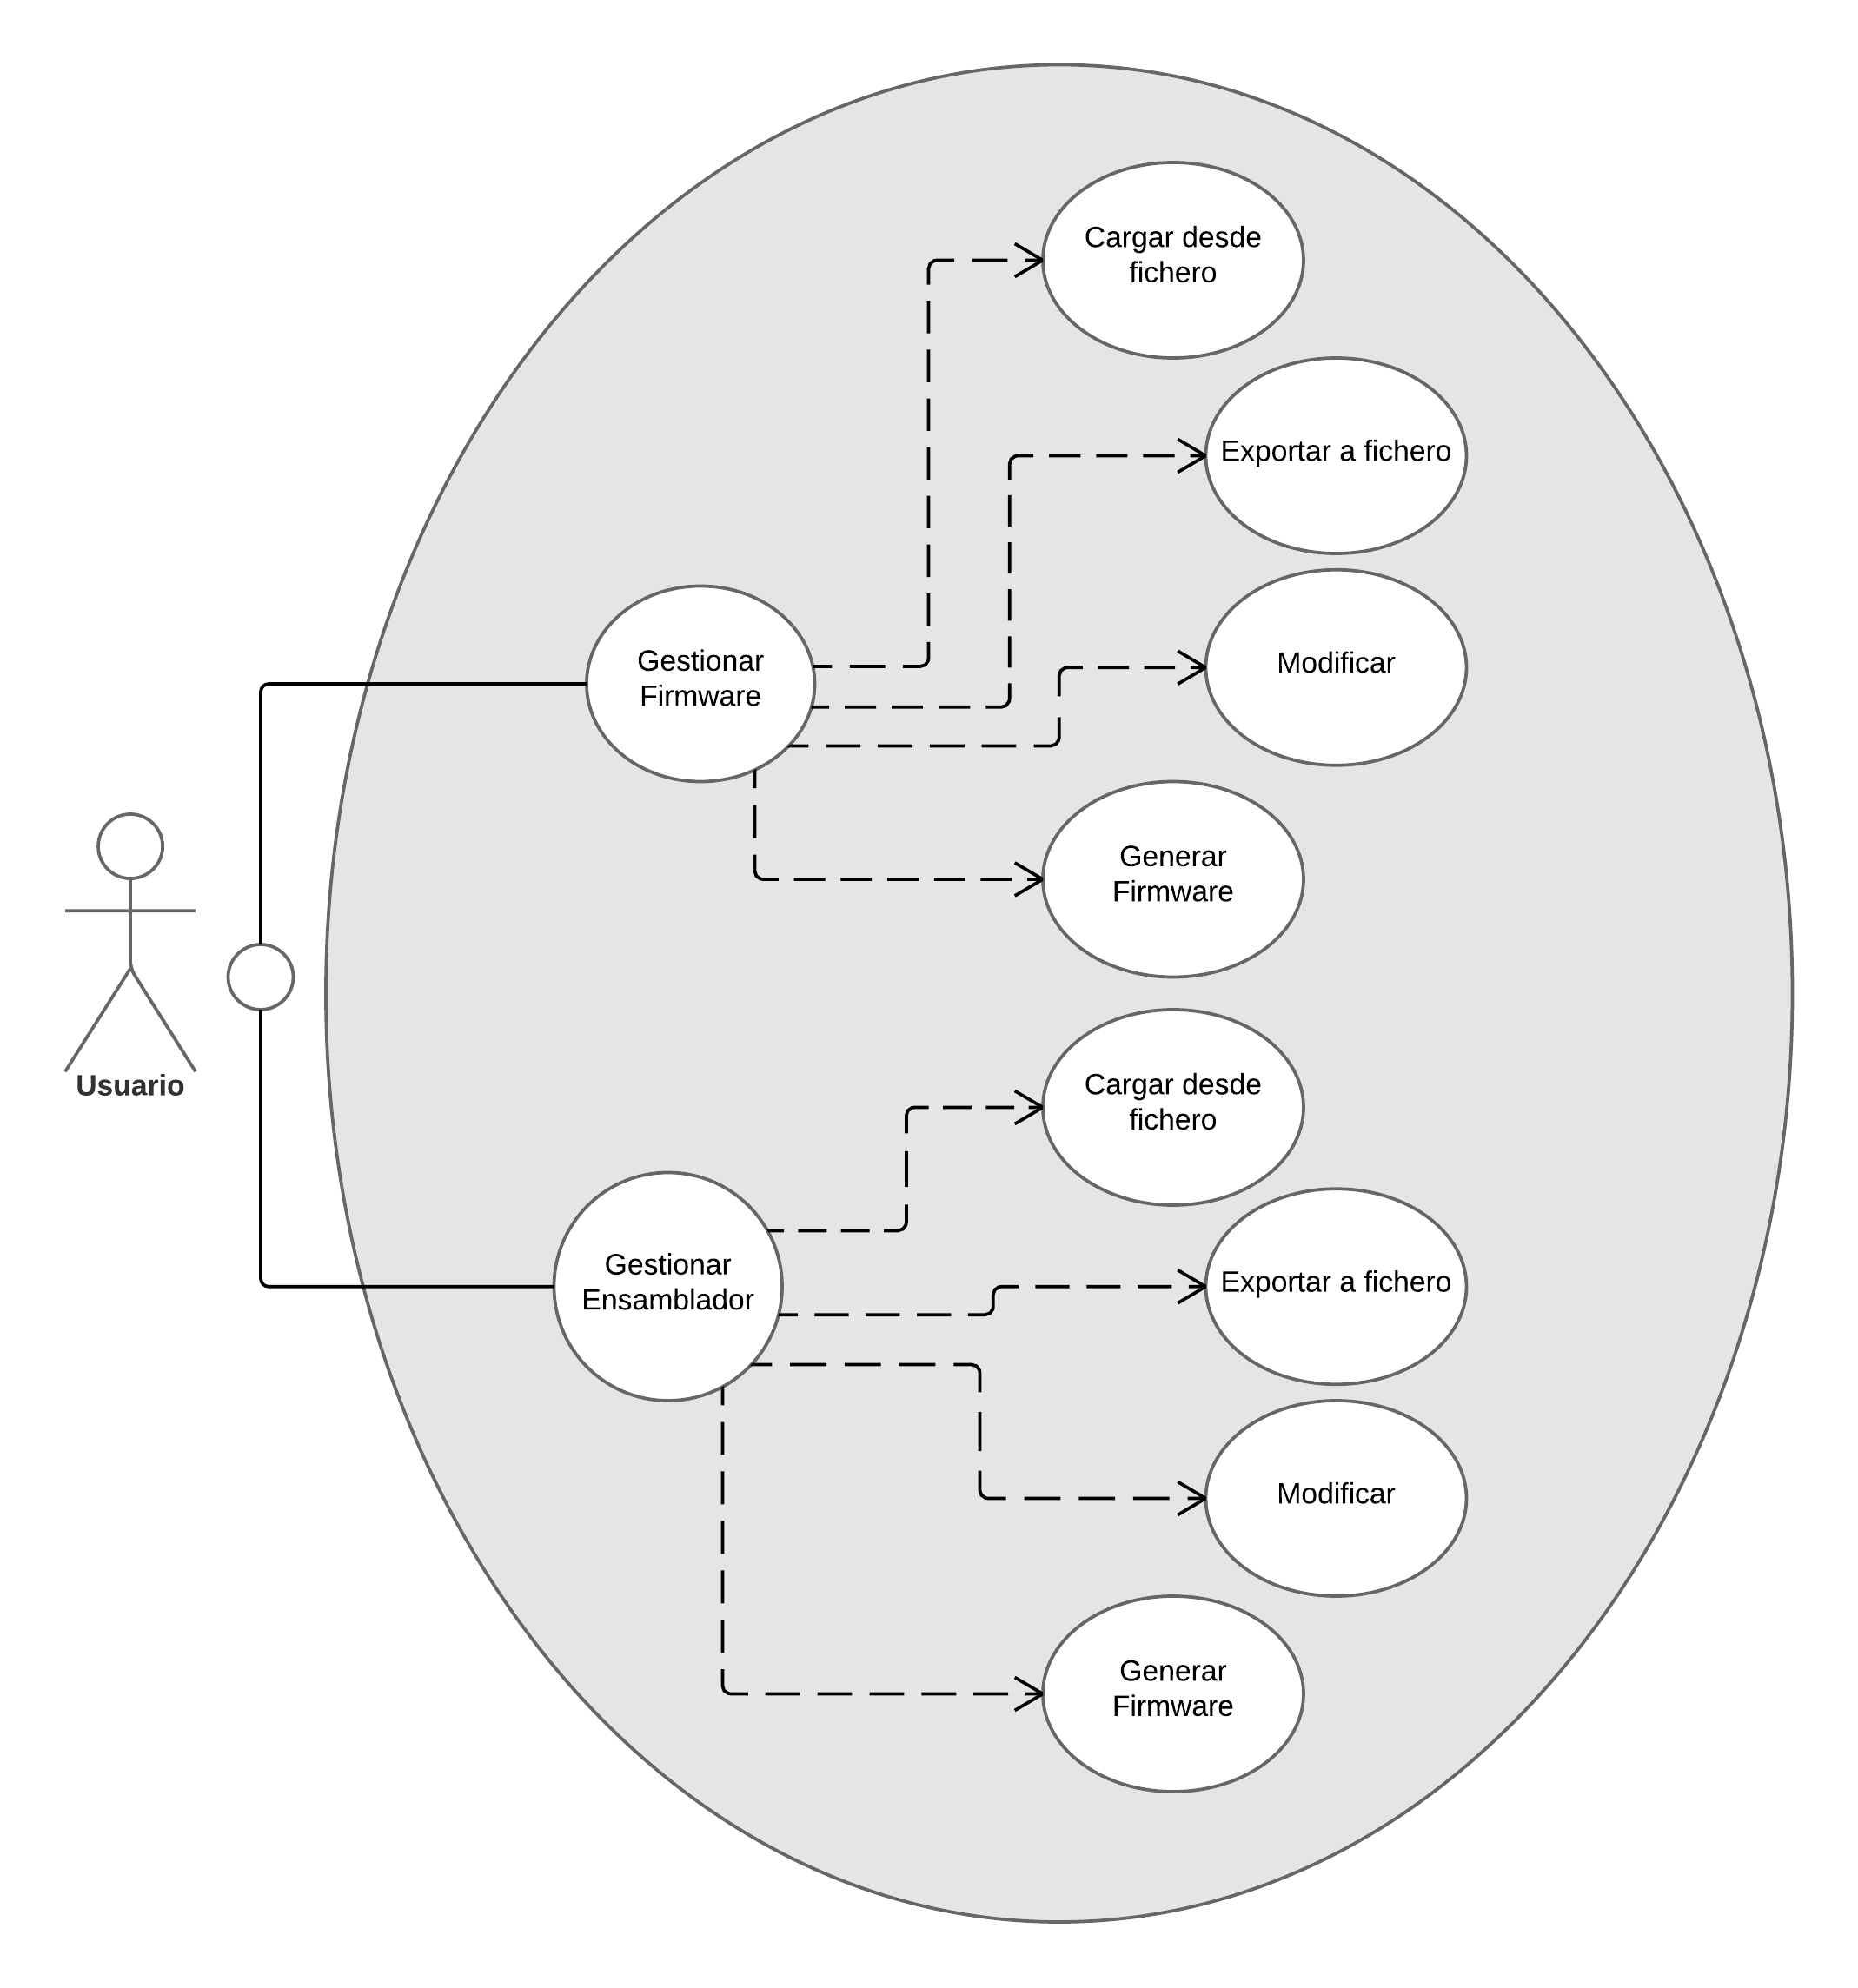
\includegraphics[width=15cm]{figures/user_cases_1}
 	\caption{Diagrama Modelo Casos de Uso 1.}
	\label{fig:user_cases1}
\end{figure}

\vspace{10 mm}

\begin{figure}[htbp]
 	\centering
 	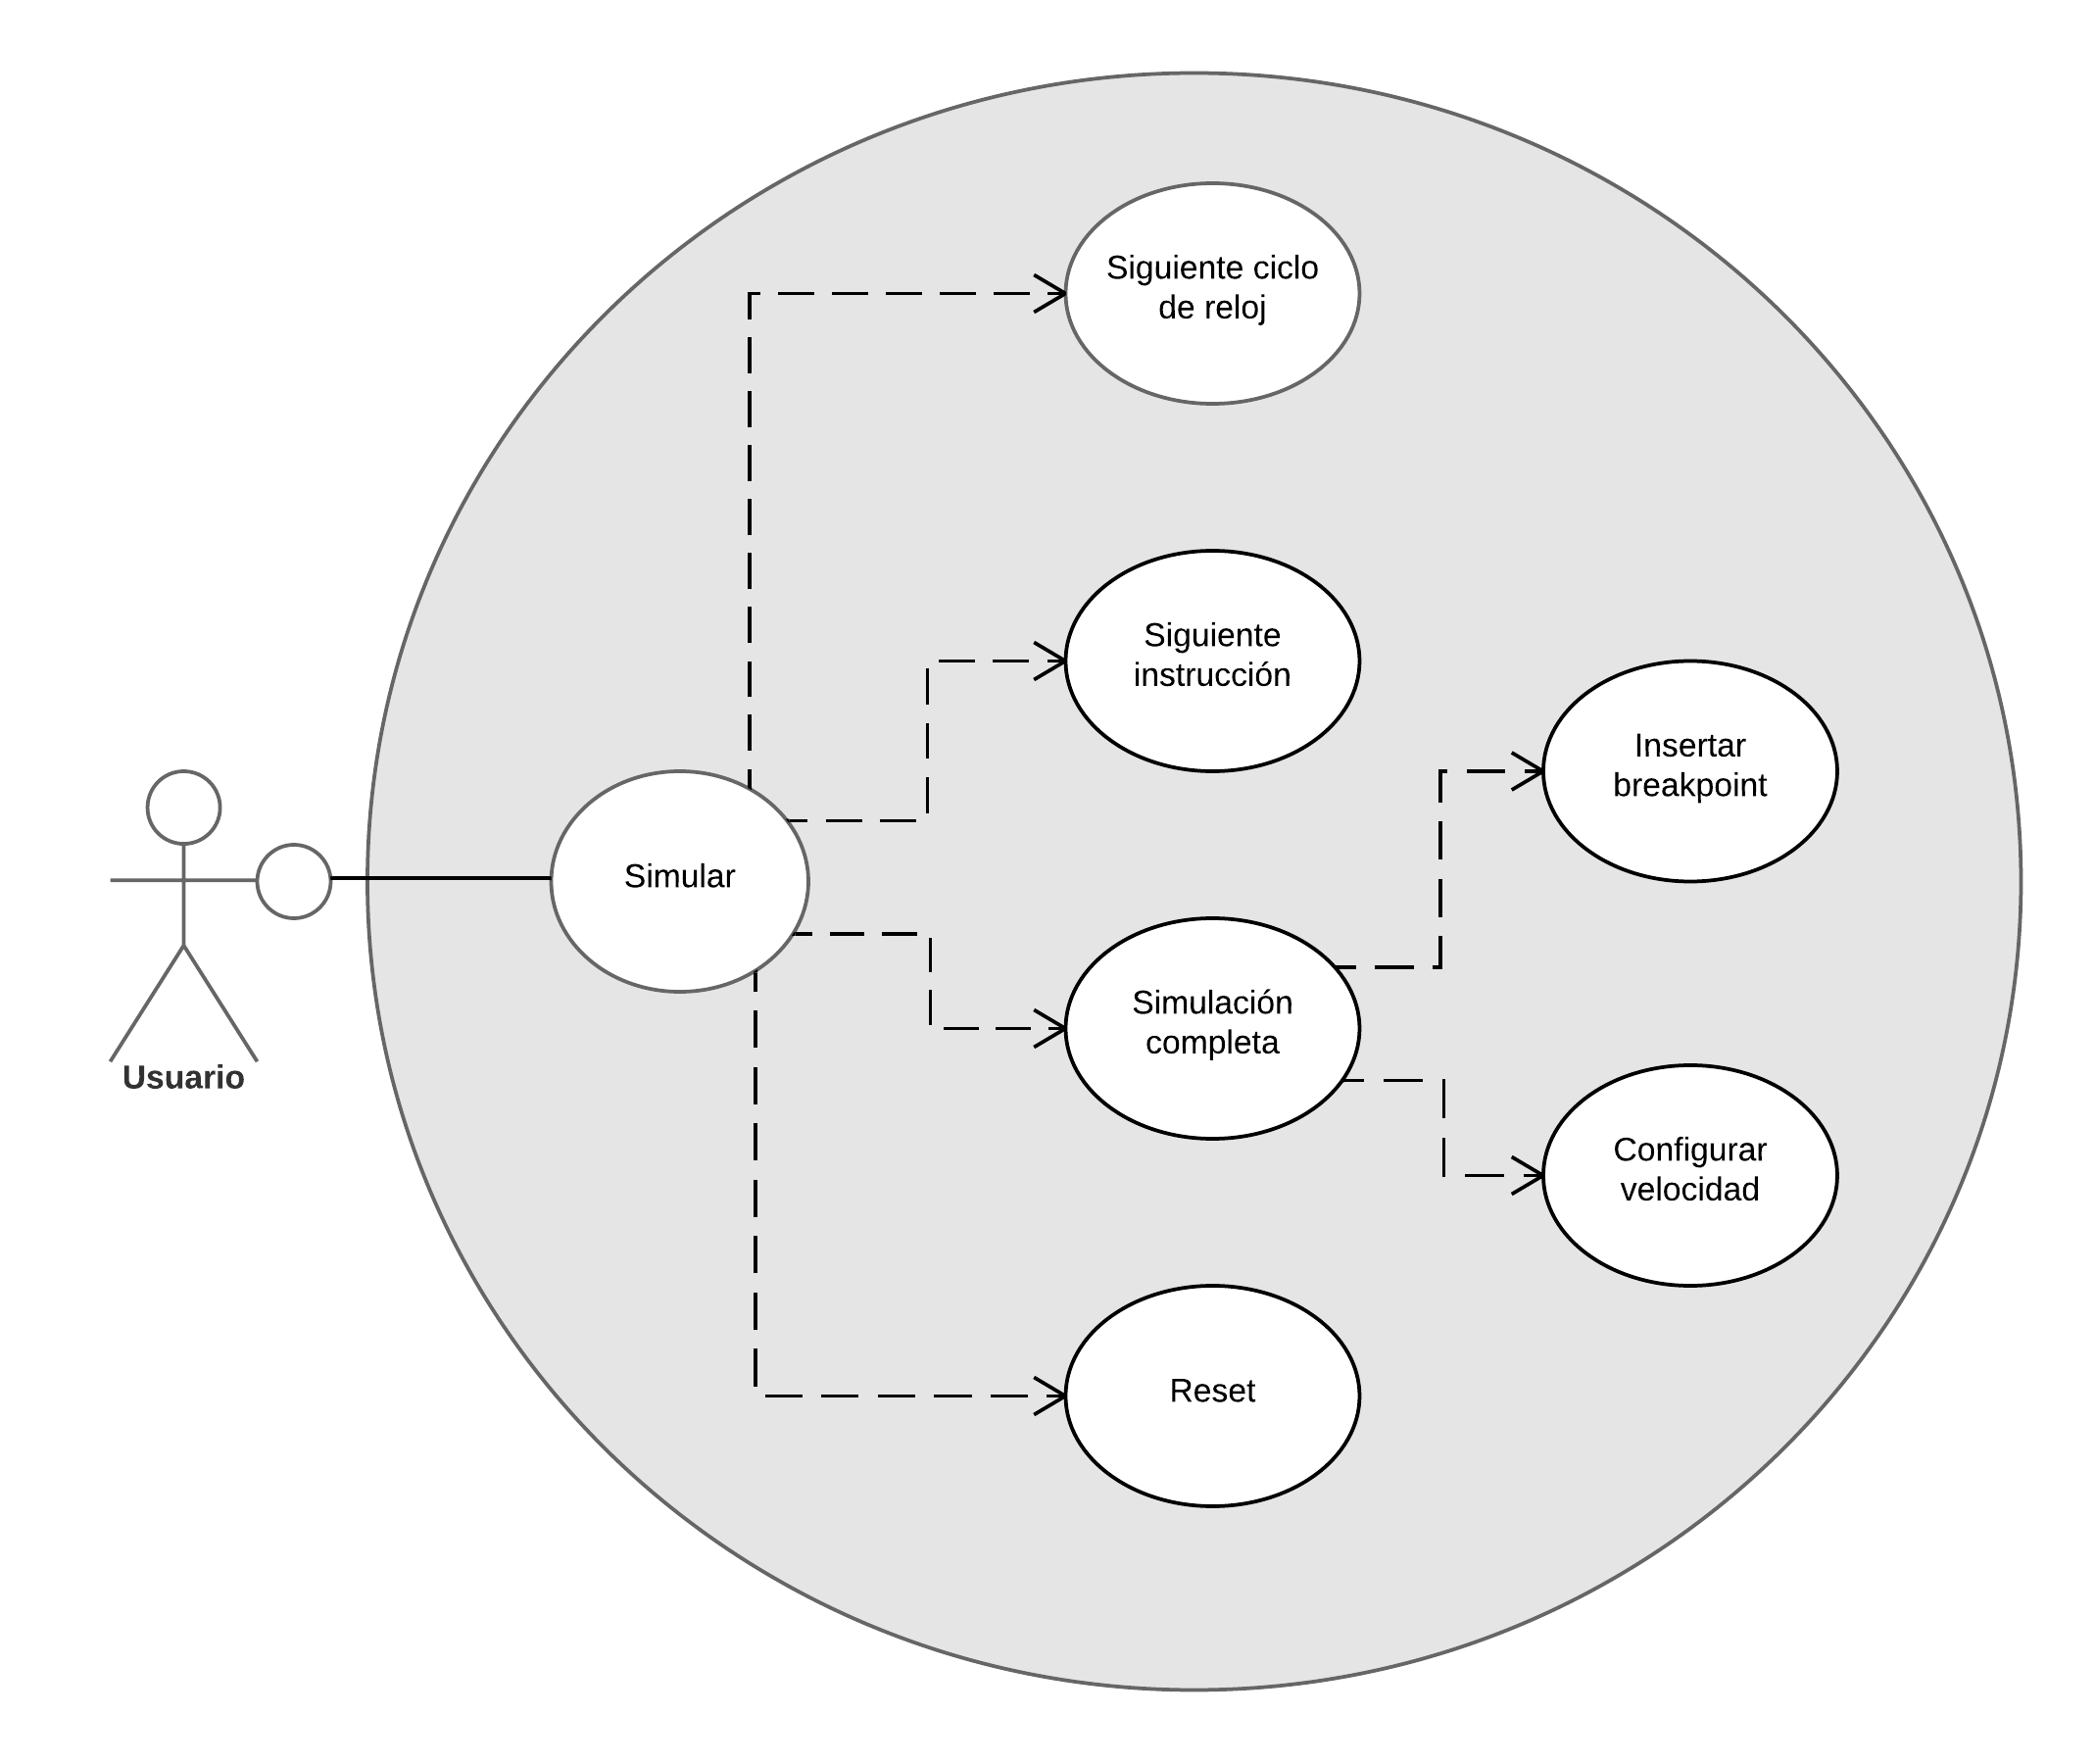
\includegraphics[width=15cm]{figures/user_cases_2}
 	\caption{Diagrama Modelo Casos de Uso 2.}
	\label{fig:user_cases2}
\end{figure}

Para realizar la especificación clara, completa y detallada de cada uno de los casos de uso recogidos en el diagrama anterior se utilizará una tabla donde se recogerán los siguientes campos de información.

\begin{center}
\begin{table*}[htbp]
\centering
\begin{tabular}{@{}p{2.5cm} p{9cm}@{}} 
\toprule
\textbf{ID}	& Caso de Uso ID.  \\
\midrule
\textbf{Nombre} 		& Nombre del Caso de Uso.   \\
\midrule
\textbf{Actores} 		&	Describe el actor o los actores que intervienen en la realización del caso de uso.  \\
\midrule
\textbf{Objetivo} 	&	Describe textualmente el cometido concreto del caso de uso. 	 \\
\midrule
\textbf{Precondiciones}	&	Muestra el estado del sistema que debe darse para que se pueda realizar el caso de uso.   \\
\midrule
\textbf{Postcondiciones} 	&	Presenta el estado del sistema tras la realización del caso de uso.   \\
\midrule
\textbf{Escenario Básico} 	&  Especifica la secuencia de pasos principales que se efectúan para realizar el caso de uso. \\
\bottomrule
\end{tabular}
\caption{Plantilla de caso de uso.}
\label{tab:uc_template}
\end{table*}
\end{center}

La tabla \ref{tab:uc_template} proporciona la plantilla utilizada para la especificación de casos de uso. Tenga en cuenta que el formato de identificación será UC-XX, donde XX corresponde al número de caso de uso. 

\begin{center}
\begin{table*}[htbp]
\centering
\begin{tabular}{@{}p{2.5cm} p{9cm}@{}} 
\toprule
\textbf{ID}	& UC-01.  \\
\midrule
\textbf{Nombre} 		& X   \\
\midrule
\textbf{Actores} 		&	X  \\
\midrule
\textbf{Objetivo} 	&	X 	 \\
\midrule
\textbf{Precondiciones}	&	X   \\
\midrule
\textbf{Postcondiciones} 	&	X   \\
\midrule
\textbf{Escenario Básico} 	&  X \\
\bottomrule
\end{tabular}
\caption{Caso de Uso UC-01.}
\label{tab:uc01}
\end{table*}
\end{center}

\section{Marco Regulador}
\label{sec:regulatory_framework}

Esta sección discute las restricciones necesarias teniendo en cuenta el marco regulador. En concreto, se especifican las restricciones legales aplicables al simulador.

\subsection{Restricciones Legales}
\label{sec:legal_constraints}

Para el uso de la mayoría de herramientas web, los usuarios deben de registrarse, y las bases de datos de las mismas manejan información confidencial de los usuarios, por lo que es necesario garantizar que terceros no puedan acceder a esa información. Una solución es cifrar la información transmitida mediante algún \gls{protocol} criptografico. En España, este requisito es especificado en el artículo 104 del RD 1720/2007 \cite{boe2008}, que se ocupa de la Ley Española de Protección de Datos.


En contraste, la aplicación desarrollada no utiliza datos privados de los usuarios y tampoco transmite información confidencial a terceros, ya que es un simulador que únicamente utiliza los códigos generados por el usuario para ejecutarlos de forma local en la máquina del usuario.


Por otro lado, es crucial que nuestro simulador esté disponible como un software de código abierto. Queremos que sea tal que cualquiera pueda redistribuir el código o modificarlo por los términos de la Licencia Pública General Menor de GNU (LGPL) \cite{gnulgpl}. Para ello, nuestro simulador está disponible en el siguiente sitio web: 

\url{https://www.arcos.inf.uc3m.es/~wepsim/}.

\afterpage{\blankpage} % blank page
\lhead[\thepage]{CAPÍTULO \thechapter. DISEÑO}
\chead[]{}
\rhead[WepSIM: Simulador de un procesador elemental con unidad de control microprogramada\leftmark]{\thepage}
\renewcommand{\headrulewidth}{0.5pt}

\lfoot[]{}
\cfoot[]{}
\rfoot[]{}
\renewcommand{\footrulewidth}{0pt}

%% This is an example first chapter.  You should put chapter/appendix that you
%% write into a separate file, and add a line \include{yourfilename} to
%% main.tex, where `yourfilename.tex' is the name of the chapter/appendix file.
%% You can process specific files by typing their names in at the 
%% \files=
%% prompt when you run the file main.tex through LaTeX.
\chapter{Diseño}
\label{ch:design}
\markboth{}{DESIGN}

En este capítulo se realiza una descripción completa del simulador desarrollado, incluyendo la arquitectura interna y los diferentes componentes software, que componen la herramienta descritos con anterioridad en \cite{mateos2016wepsim}.

La sección \ref{sec:study_of_solution} discute el estudio de la solución final, considerando las diferentes alternativas existentes para el diseño y desarrollo del simulador. En la sección \ref{sec:solution_selection} se indica la solución elegida y la compara con las alternativas consideradas. La sección \ref{sec:simulator_architecture} describe cada uno de los componentes que componen el simulador.

\section{Estudio de la solución final}
\label{sec:study_of_solution}

Debido a los requisitos de usuario establecidos en este proyecto (Sección \ref{sec:user_requirements}), en donde se especificaba que el software no debía de ser instalado en el dispositivo del usuario, y debía de poder ser ejecutado en los navegadores web indicados, se ha decidido que el diseño del simulador esté enfocado como una aplicación web.

Existen diferentes modelos arquitectónicos a la hora de realizar el diseño de una aplicación web. La primera opción, es el modelo cliente-servidor en el cual las tareas se reparten entre dos roles: un proveedor que proporciona recursos o servicios que es llamado servidor, y un consumidor que contacta con el servidor con el objetivo de hacer uso de los recursos que este provee. Es un modelo distribuido en el que la lógica de negocio y el cómputo recae en el servidor, y el cliente provee la interfaz de usuario, realizando validaciones y procesos menores de la lógica de negocio. La segunda opción, es un modelo en el que toda la aplicación es ejecutada en el cliente, siendo únicamente necesario el servidor para el acceso al código de la aplicación. Este modelo, posibilita incluso que el servidor no sea necesario en el caso de existir el código de la aplicación web en el cliente, pudiendo ser ejecutada sin la necesidad de internet. Ambos modelos, poseen una alta compatiblidad al hacer que las aplicaciones no sean dependientes del sistema operativo del usuario, sino del navegador web que este utiliza.

Debido a los requisitos de usuario establecidos en este proyecto (Sección \ref{sec:user_requirements}), la segunda opción es la que cumple con la necesidad de no necesitar acceso a internet, de forma que la funcionalidad total del simulador quede en el dispositivo del usuario.

Una vez decidido el modelo de diseño, es necesario tener en cuenta las diferentes tecnologías a utilizar. Como se indicó en (Sección \ref{sec:user_requirements}), es necesario que la aplicación sea diseñada siguiendo el lenguaje de programación HTML5, que está formado por HTML, CSS y JavaScript. De este modo, es necesario contemplar los diferentes frameworks y bibliotecas existentes que ayudan a la hora de realizar el diseño de la aplicación, posibilitando el funcionamiento de esta tanto el ordenadores como en dispositivos móviles. Estas tecnologías descritas anteriormente en el Apartado \ref{sec:tecnologias_web}, proporcionan distintas funcionalidades y enfoques a la hora de diseñar la aplicación, permitiendo la compatibilidad de la aplicación con la amplia mayoría de los navegadores web. En la Tabla \ref{tab:comparison_webframeworks}, se analizan las funcionalidades y compatibilidades que proporcionan estas tecnologías, valorando si cumplen con los requisitos establecidos en este proyecto.

\begin{table}[htbp]
\ra{1.2}
\centering
%\resizebox{\textwidth}{%
\resizebox{\textwidth}{!}{
\begin{tabular}{@{}llllllll@{}}
\toprule
Framework & Angular.js & jQuery.js & BootStrap & Dojo \\ 
\midrule
Funcionalidad requerida			& \ding{51}  &  \ding{51} & \ding{51} & \ding{51} \\
\midrule
Ejecución en cliente				& \ding{51} & \ding{51} & \ding{51} &  \\
\midrule
Compatibilidad navegadores requeridos				& \ding{51} & \ding{51} & \ding{51} & \ding{51} \\
\midrule
Soporte plataformas móviles				& \ding{51}  & \ding{51}  & \ding{51}  & \\
\bottomrule
\end{tabular}
}
\caption{Comparación de frameworks y bibliotecas.}
\label{tab:comparison_webframeworks}
\end{table}

De este modo, se puede observar como pese a que \textit{Angular.js} nos proporciona la mayoría de funcionalidades requeridas, tiene una curva de aprendizaje bastante mayor que \textit{jQuery}, lo cual hace que \textit{jQuery} se imponga a la hora de su elección debido a que la ganancia de uso que proporcionaría \textit{Angular.js} es inferior a este inconveniente. Por otro lado, sería interesante el uso de \textit{Dojo} a la hora de utilizar una tecnología que nos proporcione funcionalidad y efectos en la interfaz de usuario y nos ayude a la capturación de eventos, pero queda descartado al estar enfocado a aplicaciones que utilizan \textit{AJAX}. De esta forma, \textit{BootStrap} será la tecnología elegida para dotar a la aplicación de la funcionalidad requerida a nivel de interfaz de usuario y complementando tanto a JavaScript como a jQuery.

\subsection{Solución elegida}
\label{sec:solution_selection}

Para que los profesores de la asignatura Estructura de Computadores puedan hacer uso de una herramienta que sirva de ayuda para la explicación de los conceptos teóricos de la asignatura, y los estudiantes puedan utilizarla para comprender estos conceptos y realizar posteriormente las prácticas de la asignatura, se propone el diseño e implementación de una herramienta web que simule con realismo en funcionamiento de un procesador elemental con unidad de control microprogramable.

Este simulador, será desarrollado como una herramienta web debido a la portabilidad que proporciona, ya que podrá ser ejecutado sobre un gran número de diferentes dispositivos independientemente del sistema operativo que utilice, puesto que únicamente necesita un navegador web para su correcto funcionamiento. De esta forma, los profesores y estudiantes podrán hacer uso de la herramienta sin depender de su instalación en el dispositivo a utilizar, incluso pudiendo los estudiantes realizar las prácticas sobre dispositivos móviles.

Para lograr dicha portabilidad, el simulador ha sido desarrollado en HTML5 (HTML + JavaScript + CSS) haciendo posible su ejecución en cualquier plataforma (smartphones, tablet, PC, etc.) que pueden ejecutar Microsoft Edge, Mozilla Firefox, Google Chrome o Safari. Además, la herramienta depende de los siguientes frameworks/bibliotecas: JQuery, JQueryUI, JQuery Mobile, Knockout y BootStrap.

Por tanto, la solución elegida es capaz de unificar en una misma herramienta todas las funcionalidades requeridas para la enseñanza de Estructura de computadores con un alto nivel de detalle, con alta disponibilidad al facilitarse su como una herramienta web, y con una gran portabilidad puesto que podrá ser ejecutada sobre un gran número de diversos dispositivos, buscando en todo momento una solución sin la necesidad de servidor.

\section{Arquitectura de WepSIM}
\label{sec:simulator_architecture}

La arquitectura de la solución presentada en este trabajo consta de tres elementos principales:

\begin{itemize}
\item Modelo hardware: permite definir el hardware a usar.
\item Modelo software: permite definir el juego de instrucciones a utilizar.
\item Kernel de simulación: simula el funcionamiento del hardware ejecutando el microcódigo/lenguaje máquina definido con anterioridad.
\end{itemize}

El modelo hardware permite definir los distintos elementos típicos de un computador (memoria principal, procesador, etc.) de una forma modular. La forma de definir estos elementos equilibra dos objetivos contrapuestos: es suficientemente completa como para imitar los principales aspectos de la realidad, pero es lo suficientemente mínima para facilitar su uso. Ante todo se persigue que sea una herramienta didáctica.

El modelo software permite definir el microcódigo y el ensamblador basado en este microcódigo de la forma tan intuitiva posible. El ensamblador a usar viene dado por un conjunto de instrucciones que puede ser definido por el usuario e intenta ser lo suficientemente flexible como para poder definir diferentes tipos y juegos de instrucciones, como por ejemplo MIPS o ARM.

El tercer elemento de la arquitectura propuesta es un kernel que toma como entrada el modelo hardware descrito y el modelo software de trabajo, y se encarga de mostrar el funcionamiento del hardware con el software dado.

\begin{figure}[htbp]
 	\centering
 	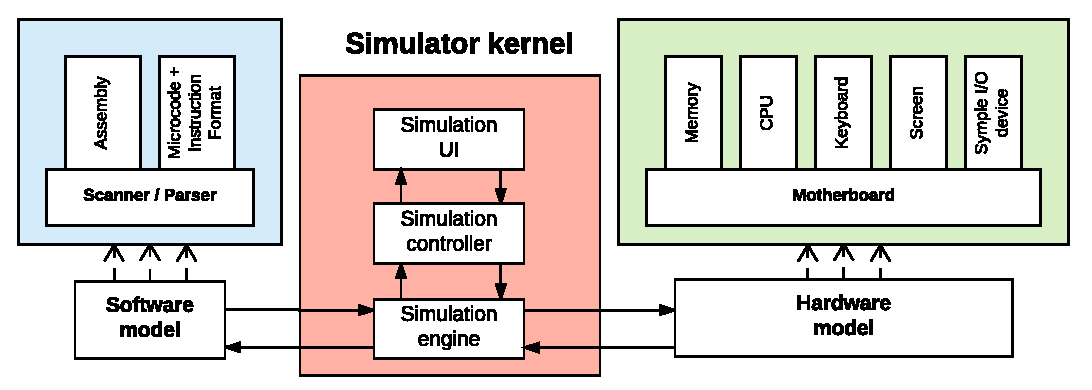
\includegraphics[width=14cm]{figures/architecture_diagram}
 	\caption{Arquitectura de WepSIM.}
	\label{fig:architecture_diagram}
\end{figure}

La figura \ref{fig:architecture_diagram} resume la arquitectura de WepSIM. El punto de inicio es el modelo hardware que describe el procesador a ser simulado. Ello incluye el procesador, la memoria y algunos dispositivos de E/S: teclado, pantalla y un dispositivo de E/S simple que genera interrupciones. El modelo hardware describe el estado global del procesador. A partir del estado global del procesador, el kernel de simulación actualiza el estado en cada ciclo de reloj.

La unidad de control simulada almacena las señales de control de cada ciclo en una memoria de control. La memoria de control tiene todos los microprogramas para las instrucciones con las que trabaja el procesador, y el fetch para leer la instrucción de memoria y decodificarla.


El microcódigo (el contenido de la memoria de control) junto con el formato de cada instrucción (campos de la instrucción y su longitud) se describe en un fichero de texto. El modelo software lee este fichero, lo traduce a binario y lo carga en el procesador. La definición del lenguaje ensamblador a utilizar se describe junto con el microcódigo, y el modelo software permite traducir a binario programas escritos en dicho ensamblador.


El kernel de simulación pregunta al subsistema del modelo software por el microcódigo definido, la descripción del formato de instrucción y el contenido de la memoria principal. Los binarios se cargan en los elementos del modelo hardware, y a continuación el kernel de simulación actualiza el estado global en cada ciclo de reloj.


WepSIM dispone de un controlador de simulación que se encarga de actualizar el ciclo de reloj y mostrar el estado global. El subsistema de interfaz de simulación actualiza la interfaz de usuario. Cuando el usuario usa la interfaz de usuario para solicitar una operación, el subsistema de interfaz de simulación traslada la petición al controlador de simulación. Como se puede ver, se usa un Modelo- Vista-Controlador (MVC) básico para la arquitectura de WepSIM.

\subsection{Modelo hardware}

El modelo hardware que usa WepSIM permite definir los distintos elementos típicos de un computador (memoria principal, procesador, etc.) de una forma modular y de manera que sea posible añadir, quitar o modificar estos elementos.

\begin{figure}[htbp]
 	\centering
 	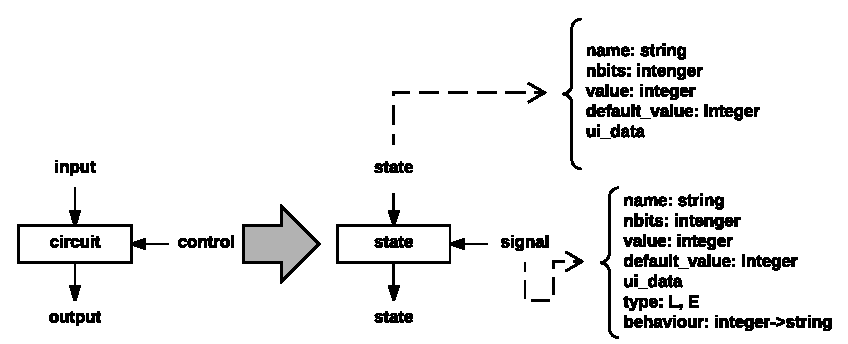
\includegraphics[width=14cm]{figures/hardware_model}
 	\caption{Modelado del hardware.}
	\label{fig:hardware_model_diagram}
\end{figure}

La figura \ref{fig:hardware_model_diagram} introduce el modelo propuesto. Cada elemento del circuito se describe como una caja negra con posibles entradas, posibles salidas y señales de control (que controlan las posibles transformaciones de las entradas a las salidas). El subsistema del modelo hardware transforma esta caja negra en dos conjuntos de objetos: estados y señales. Un estado tiene un identificador (el nombre), el valor (un valor entero) y un valor inicial (el valor por defecto). Los valores que puede tomar son valores naturales dentro de un rango, dado por el número de bits con los que se representa el estado. Una señal es un estado especial que controla el valor de otros estados o señales. Hay dos atributos asociados a las señales (y no a los estados): el tipo de señal (por nivel o por flanco) y su comportamiento. Para cada valor de señal una cadena de caracteres describe en un Lenguaje Simple lo que la señal mueve o transforma. Este Lenguaje Simple se compone principalmente de instrucciones que representan las operaciones elementales.

\begin{figure}[htbp]
 	\centering
 	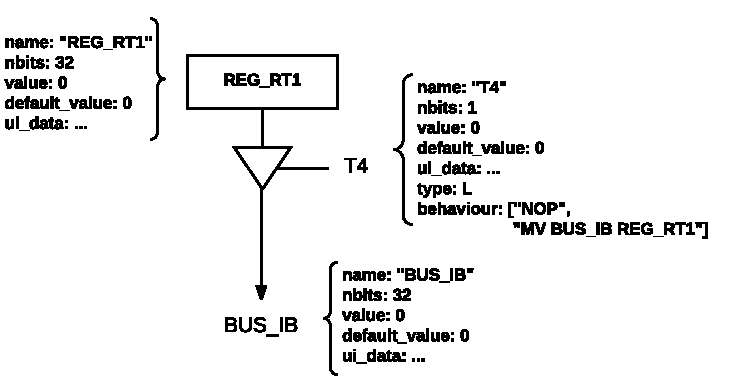
\includegraphics[width=14cm]{figures/hardware_example_tristate}
 	\caption{Ejemplo de modelado de una puerta triestado.}
	\label{fig:hardware_tristate_example}
\end{figure}

\begin{figure}[htbp]
 	\centering
 	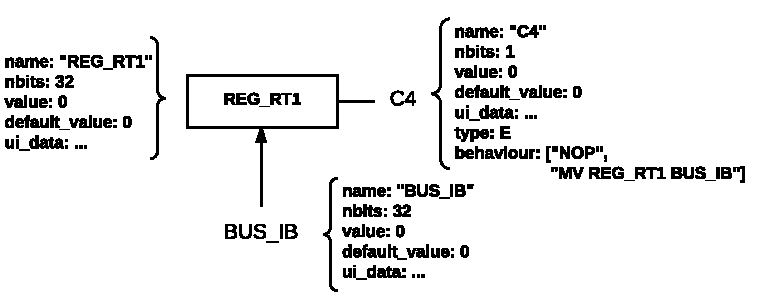
\includegraphics[width=14cm]{figures/hardware_example_register}
 	\caption{Ejemplo de modelado de un registro.}
	\label{fig:hardware_register_example}
\end{figure}

Las figuras \ref{fig:hardware_tristate_example} y \ref{fig:hardware_register_example} muestran dos ejemplos: un triestado y un registro.
El triestado controla dos estados: el estado del bus al que se conecta BUS IB y el estado del registro de entrada, REG RT1 en este caso. Ambos representan el valor a la salida de la puerta (BUS IB) y el valor del registro RT1 (REG RT1). La señal T4 se encarga de indicar cuándo el valor del registro RT1 se envía a la salida. Esta señal T4 es una señal por nivel (tipo: L), con valor cero no tiene efecto (comportamiento ``NOP''). Cuando el valor de la señal es uno entonces el comportamiento es el de copiar el valor del registro RT1 a la salida (comportamiento ``MV BUS IB REG RT1'').

El ejemplo con el registro (figura \ref{fig:hardware_register_example}) es similar. En este caso trabaja con dos estados: el contenido del registro RT1 y el contenido situado a la entrada (BUS IB). La señal C4 controla cuándo se almacena en el registro RT1 el valor que hay en la entrada. La diferencia está en el tipo de señal: C4 es una señal por flanco de bajada (tipo: E), por lo que al final del ciclo de reloj (pasa de uno a cero) si la señal vale uno entonces el comportamiento es el de copiar el valor situado a la entrada al registro (comportamiento ``MV REG RT1 BUS IB'').

El Lenguaje Simple usado para definir los comportamientos añade a las operaciones elementales otras operaciones necesarias. Por ejemplo disparar una señal (``FIRE C4'') que ayuda a propagar el efecto de una señal al revaluar la señal inmediata que podría verse afectada. Otro ejemplo lo encontramos en dos operaciones que pueden ser muy útiles a la hora de depurar: imprimir el valor de un estado (``PRINT E BUS IB'') e imprimir el valor de una señal (``PRINT S C4'').

\subsection{Modelo software}

Una vez definido el procesador elemental usando el modelo hardware propuesto, toca describir el conjunto de instrucciones que es capaz de ejecutar así como el microcódigo que lo orquesta. En un fichero de texto se define el formato de las instrucciones máquina junto con el cronograma asociado a la ejecución de cada una de las instrucciones máquina. La figura \ref{fig:software_format_example} muestra un ejemplo de definición para la instrucción li (load inmmediate), que almacena un valor inmediato en un registro.

\begin{figure}[htbp]
 	\centering
 	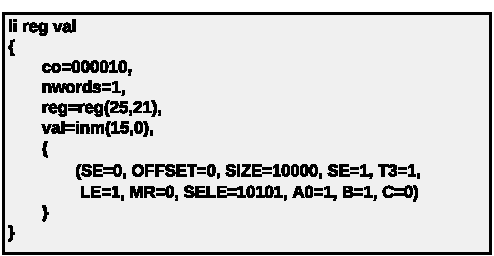
\includegraphics[width=10cm]{figures/instruction_example}
 	\caption{Ejemplo de formato de instrucción.}
	\label{fig:software_format_example}
\end{figure}

\vspace{10mm}

El fichero con el cronograma de fetch y todos los cronogramas de las instrucciones define el microcódigo para la plataforma WepSIM. El simulador permite la definición de diferentes juegos y formatos de instrucciones. Inicialmente se ha implementado un subconjunto de las instrucciones del MIPS, pero es posible definir instrucciones de otros conjuntos de forma similar. En este fichero se pueden asignar códigos simbólicos a los registros del banco de registros, lo que permite que en los programas escritos en ensamblador se puedan usar dichos  símbolos (por ejemplo, registro \$t3 en la figura \ref{fig:software_assembly_example}).

\begin{figure}[htbp]
 	\centering
 	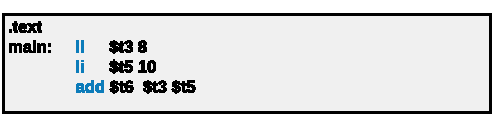
\includegraphics[width=10cm]{figures/example_assembly}
 	\caption{Ejemplo de código fuente en ensamblador.}
	\label{fig:software_assembly_example}
\end{figure}

El campo “co” identifica el código de instrucción máquina, que es un número binario de 6 bits. Esto permite definir hasta 64 instrucciones distintas. Dado que los últimos 4 bits de la instrucción pueden usarse para seleccionar la operación en la ALU, es posible seleccionar hasta 16 operaciones aritmético-lógicas con un mismo código de instrucción, por lo que se podrían tener 79 (63+16) instrucciones en total.

Cuando WepSIM carga el microcódigo, cada código de instrucción tiene asociado una dirección de comienzo en la memoria de control donde se almacena el cronograma asociado. Esta tabla con dos columnas (el código de instrucción y su dirección de comienzo asociada en la memoria de control) se carga en la ROM co2microAddr mostrada en la figura \ref{fig:wepsimCU_figure}.

El campo ``nwords'' define cuantas palabras precisa la instrucción para su definición y carga en memoria. Una palabra en WepSIM son 4 bytes.

Para cada campo de la instrucción se define el bit inicial, el bit final (ambos incluidos) y el tipo de campo (registro, valor inmediato, dirección absoluta y dirección relativa a PC). Una vez definido el formato, se definen todas las microinstrucciones que necesita la instrucción máquina definida para su ejecución. Todas las microinstrucciones se encuentran encerradas entre llaves y cada microinstrucción está formada por una lista de tuplas (señal, valor) encerradas entre paréntesis. Para la instrucción definida en la figura \ref{fig:software_format_example} se precisa de una sola microinstrucción, en la que se indican qué señales se activan durante un ciclo de reloj. Para las señales no indicadas se asume que su valor es 0 durante el ciclo de reloj correspondiente.

Una vez cargado el microcódigo en WepSIM, es posible cargar cualquier fichero ensamblador que haya sido codificado usando las instrucciones  máquina definidas anteriormente en el microcódigo.

En la figura \ref{fig:software_assembly_example} se muestra un ejemplo de código fuente en ensamblador que se puede usar en WepSIM. Este ejemplo en particular muestra un código estilo MIPS. Para que un programa en ensamblador pueda utilizar la instrucción de carga inmediata li (load inmmediate) y de suma add (addition), deben haber sido definidas previamente en el microcódigo. WepSIM puede comprobar los errores de sintaxis y construir el binario mediante el rellenado de los campos descritos en la definición del microcódigo correspondiente a la instrucción. La figura \ref{fig:software_assembly_traduction} muestra un ejemplo de traducción a binario para la instrucción li \$2 5 en función del formato definido en la figura \ref{fig:software_format_example}. También se debe haber definido en el fichero de microcódigo el valor del registro asociado a la etiqueta \$2 (00100 en este caso).

\begin{figure}[htbp]
 	\centering
 	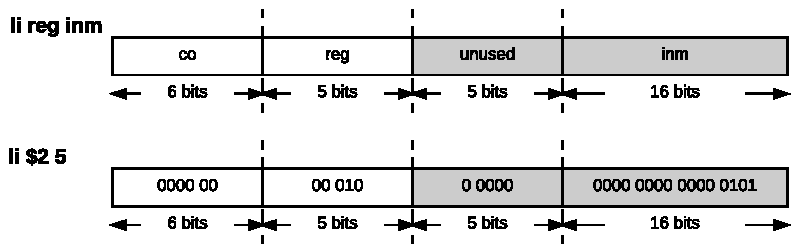
\includegraphics[width=14cm]{figures/instruction_example_traduction}
 	\caption{Formato de instrucción descrito en el microcódigo y ejemplo de su traducción en binario.}
	\label{fig:software_assembly_traduction}
\end{figure}

Una de las grandes ventajas del simulador WepSIM es que no está limitado a un conjunto de instrucciones concreto. Se puede definir un amplio conjunto de instrucciones de procesadores reales o inventados. Se puede usar para añadir por ejemplo, a un conjunto de instrucciones MIPS, otras instrucciones diferentes no incluidas en dicho conjunto de instrucciones.

\subsection{Kernel del simulador}
\label{sec:kernel_simulator}

El kernel del simulador, es el componente que integra la interfaz de usuario del simulador, el controlador del simulador, y el motor de simulación, siendo el encargado de hacer las funciones de controlador de la herramienta gestionando las comunicaciones de la interfaz de usuario con los modelos hardware y software. 

De esta forma cuando el usuario interacciona con la interfaz gráfica, el módulo encargado de la interfaz genera eventos que identifican las acciones que el usuario realiza. Estos eventos son generados a modo de peticiones al controlador de la simulación, que se encarga de identificar el evento generado, comprobar el contexto en el cual se encuentra, y enviar la acción correspondiente a realizar al motor del simulador. El motor del simulador, se encarga de comunicarse con los modelos hardware y software, de forma que estos puedan ejecutar correctamente la acción solicitada (Figura \ref{fig:kernel_diagram}).

\begin{figure}[htbp]
 	\centering
 	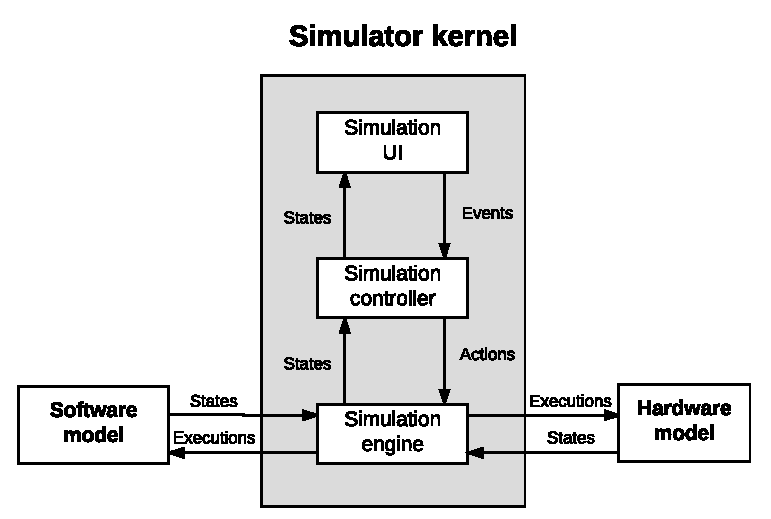
\includegraphics[width=10cm]{figures/kernel_diagram}
 	\caption{Arquitectura del kernel del simulador.}
	\label{fig:kernel_diagram}
\end{figure}

Por ejemplo, si el usuario selecciona la ejecución de un ciclo de reloj, la interfaz de usuario genera el evento correspondiente. El controlador del simulador, se encarga de identificar el evento, verificar que se cumplen todas las condiciones para poder ejecutarse un ciclo de reloj comprobando diferentes valores del estado del simulador. En caso de poder ser realizada la ejecución del ciclo de reloj, envía la orden al motor del simulador que se encarga de comunicarse con el  modelo hardware, realizando la ejecución de un ciclo de reloj actualizando los componentes del modelo hardware. Por último, la interfaz de usuario consulta el estado del modelo hardware actualizando la información necesaria para ser mostrada al usuario.





\lhead[\thepage]{CAPÍTULO \thechapter. IMPLEMENTACIÓN Y DESPLIEGUE}
\chead[]{}
\rhead[WepSIM: Simulador de procesador elemental con unidad de control microprogramada\leftmark]{\thepage}
\renewcommand{\headrulewidth}{0.5pt}

\lfoot[]{}
\cfoot[]{}
\rfoot[]{}
\renewcommand{\footrulewidth}{0pt}

%% This is an example first chapter.  You should put chapter/appendix that you
%% write into a separate file, and add a line \include{yourfilename} to
%% main.tex, where `yourfilename.tex' is the name of the chapter/appendix file.
%% You can process specific files by typing their names in at the 
%% \files=
%% prompt when you run the file main.tex through LaTeX.
\chapter{Implementación y despliegue}
\label{ch:implementation_and_deployment}
\markboth{}{IMPLEMENTATION}


Este capítulo trata de la implementación y despliegue del software. En cuanto a la implementación del sistema, se explican las partes más complicadas del código en (Sección  \ref{sec:implementation}, \textit{\nameref{sec:implementation}}). Por otro lado, explicamos los pasos necesarios para desplegar el sistema final (Sección \ref{sec:deployment}, \textit{\nameref{sec:deployment}})


\section{Implementación}
\label{sec:implementation}


Como hemos explicado en el capítulo \ref{ch:analysis}, \textit{\nameref{ch:analysis}}, hemos implementado el simulador utilizando el lenguaje de programación JavaScript junto con HTML5, CSS y las bibliotecas/frameworks JQuery, JQueryUI, JQuery Mobile, Knockout y BootStrap. El motor de simulación es el encargado de ejecutar cada uno de los ciclos de reloj del simulador, tomando como entradas tanto el modelo hardware como el modelo software, pero el desarrollador ha debido de diseñar e implementar el algoritmo que posibilita esta ejecución.

Además, hemos trabajado en conseguir una herramienta que sea capaz de generar la memoria de control mediante la definición del juego de instrucciones por parte del usuario, y de generar el código binario asociado al código ensamblador definido por el usuario; el cual depende del juego de instrucciones definido previamente. Para ello, se han diseñado e implementado dos compiladores diferentes, capaces de generar los binarios correspondientes además de las estructuras de datos necesarias para ayudar al motor de simulación a lo largo de la ejecución.

De esta forma, en \ref{alg:core_simulator_pseudocode} podemos ver el pseudocódigo de como se realiza una simulación, realizando la comprobación de segmentos de memoria, tipo de simulación, y ejecución del ciclo o instrucción correspondiente. En \ref{alg:firmware_compiler_pseudocode}, podemos observar el pseudocódigo del proceso de generación de la memoria de control, mientras que en \ref{alg:assembly_compiler_pseudocode} podemos ver el proceso de compilación del código ensamblador definido por el usuario en función de la memoria de control previamente generada.

\vspace{1cm}

\begin{algorithm}[h]
	\caption{Proceso de simulación}
	\label{alg:core_simulator_pseudocode}
  	\scriptsize
  	\setstretch{1.35}
	\begin{algorithmic}[1]
		\Function{run\_simulation}{ }
		  \If {(!possible\_execute())}
		    \State Return;
		  \EndIf		
		  \State change\_play\_button();
		  \State execute\_simulation\_inchain();
		\EndFunction
		\Function{execute\_simulation\_inchain}{ }
		   \If {(end\_code())}
		    \State Return;
		   \EndIf	
		   \If {(is\_breakpoint())}
		    \State Return;
		   \EndIf	
		   \If{(execute\_mode == microInstruction)}
		         \State{execute\_microInstruction();}
		   \EndIf
		   \If{(execute\_mode == instruction)}
		         \State{execute\_instruction();}
		   \EndIf	
		\EndFunction
		\Function{execute\_microInstruction()}{ }
		\If {(!possible\_execute())}
		    \State Return;
		\EndIf
		\State compute\_general\_behaviour(CLOCK); \Comment{execute cycle}
		\State update\_UI();		
		\EndFunction
		\Function{execute\_instruction()}{ }
		\If {(!possible\_execute())}
		    \State Return;
		\EndIf
		\Do
		\State compute\_general\_behaviour(CLOCK); \Comment{execute cycle}
		\doWhile{($reg\_microaddr$!=$0$ and $mem\_control$[$microAddr$]!=$undefined$)} \Comment{check next cycle}
		\State update\_UI(); \Comment{update user interface}
		\EndFunction
	\end{algorithmic}
\end{algorithm}

\clearpage

\begin{algorithm}[h]
	\caption{Proceso de compilación del juego de instrucciones}
	\label{alg:firmware_compiler_pseudocode}
  	\scriptsize
  	\setstretch{1.35}
	\begin{algorithmic}[1]
		\Function{work\_fetch}{ }
		\State $project = null$
		\While {time < max\_time}
		\For {each project $p$ in $projects$}
		\If {$p$ meets the requirements}
		\State $project = p$
		\EndIf
		\EndFor
		\If {$project$ and not $deadlines\_missed$}
		\State \Call{ask\_for\_work}{$project$}
		\EndIf		
		\State \Call{wait}{} $work\_fetch\_period$
		\EndWhile	
		\State \Call{signal}{} Client main process
		\State Return
		\EndFunction
	\end{algorithmic}
\end{algorithm}

\begin{algorithm}[h]
	\caption{Proceso de compilación de código ensamblador}
	\label{alg:assembly_compiler_pseudocode}
  	\scriptsize
  	\setstretch{1.35}
	\begin{algorithmic}[1]
		\Function{work\_fetch}{ }
		\State $project = null$
		\While {time < max\_time}
		\For {each project $p$ in $projects$}
		\If {$p$ meets the requirements}
		\State $project = p$
		\EndIf
		\EndFor
		\If {$project$ and not $deadlines\_missed$}
		\State \Call{ask\_for\_work}{$project$}
		\EndIf		
		\State \Call{wait}{} $work\_fetch\_period$
		\EndWhile	
		\State \Call{signal}{} Client main process
		\State Return
		\EndFunction
	\end{algorithmic}
\end{algorithm}


\section{Despliegue}
\label{sec:deployment}

En esta sección se presenta el despliegue de la herramienta. Para ello, indicamos las especificaciones técnicas recomendadas para que el usuario final obtenga la mejor experiencia posible con la herramienta:

\begin{itemize}

\item \textbf{Sistema Operativo}: Ubuntu 16.04.2 LTS (Linux distribution) /Windows 10 / MacOS 10.12.5.

\item \textbf{Procesador}: Intel(R) Core(TM) i3 CPU 6300 @3.8GHz or higher.

\item \textbf{\gls{ram}}: 4 GB or higher.

\item \textbf{Almacenamiento}: 1 GB of free space in the Hard Disk Drive (recomendado para el navegador web).

\item \textbf{Red}: La conexión a internet no es necesaria para la ejecución de la herramienta, únicamente para el acceso a ella.

\item \textbf{Software}: Los siguientes navegadores web son los recomendados para el uso de la herramienta:

	\begin{itemize}

	\item[1.] Mozilla Firefox.
	
	\item[2.] Google Chrome.
	
	\item[3.] Microsoft Edge.
	
	\item[4.] Safari.

	\end{itemize}

\end{itemize}

\begin{figure}[htbp]
 	\centering
 	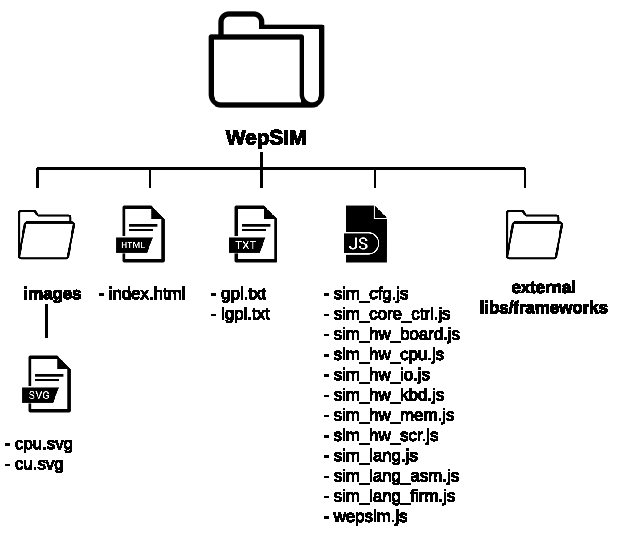
\includegraphics[width=10cm]{figures/folder_diagram}
 	\caption{Estructura de ficheros.}
	\label{fig:folder_structure}
\end{figure}

En caso de desear el usuario descargar el código fuente de la herramienta para realizar cualquier modificación en la definición del modelo hardware o cualquier otro módulo, es necesario explicar la estructura de ficheros que componen el simulador y las dependencias que existen entre sí. De esta forma, en \ref{fig:folder_structure} podemos ver los ficheros que componen la herramienta web, los cuales tienen una serie de dependencias indicadas en \ref{fig:files_dependencies}.

\begin{figure}[htbp]
 	\centering
 	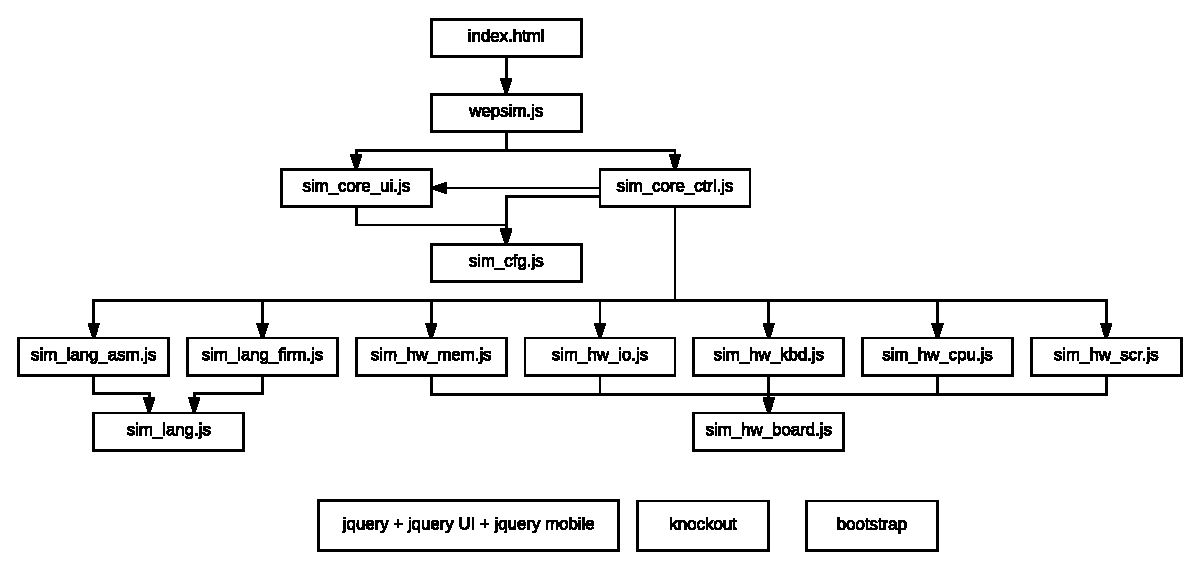
\includegraphics[width=15.5cm]{figures/dependencies_diagram}
 	\caption{Dependencias entre ficheros.}
	\label{fig:files_dependencies}
\end{figure}

Los ficheros que componen WepSIM son detallados a continuación:

\begin{itemize}

\item \textbf{index.html: } este fichero se encarga de la vista de la herramienta, generando la interfaz de usuario de la herramienta.

\item \textbf{gpl.txt y lgpl.txt: } estos ficheros contienen la especificación de las licencias del software.

\item \textbf{sim\char`_cfg.js} este fichero contiene las estructuras de datos de la configuración de la herramienta.

\item \textbf{sim\char`_core\char`_ctrl.js:}  este fichero contiene la implementación del motor de simulación de la herramienta.

\item \textbf{sim\char`_core\char`_ui.js: } este fichero contiene la implementación del motor de la interfaz de usuario de la herramienta.

\item \textbf{sim\char`_hw\char`_cpu.js: } este fichero contiene la definición del modelo hardware de la cpu del simulador.

\item \textbf{sim\char`_hw\char`_io.js: } este fichero contiene la definición del modelo hardware del módulo de generación de interrupciones del simulador.

\item \textbf{sim\char`_hw\char`_kbd.js: } este fichero contiene la definición del modelo hardware del módulo del teclado del simulador.

\item \textbf{sim\char`_hw\char`_scr.js: } este fichero contiene la definición del modelo hardware de la memoria principal del simulador.

\item \textbf{sim\char`_hw\char`_mem.js: } este fichero contiene la definición del modelo hardware de la pantalla del simulador.

\item \textbf{sim\char`_lang.js: } este fichero contiene la implementación de las funciones principales del parser de ficheros de la herramienta.

\item \textbf{sim\char`_lang\char`_asm.js: } este fichero contiene la implementación del compilador de código ensamblador de la herramienta.

\item \textbf{sim\char`_lang\char`_firm.js: } este fichero contiene la implementación del compilador de firmware de la herramienta.

\item \textbf{images/cpu.svg: } este fichero contiene la definición de la imagen vectorial de la cpu de la herramienta.

\item \textbf{images/cpu.svg: } este fichero contiene la definición de la imagen vectorial de la unidad de control de la herramienta.

\item \textbf{external folder: } este directorio contiene las bibliotecas y frameworks que necesita el simulador para su correcto funcionamiento, como son JQuery, JQueryUI, JQuery Mobile, Knockout y BootStrap.

\end{itemize}

En \cite{wepsimManualUser} se presenta el manual completo de usuario de la herramienta, que incluye la especificación del modelo hardware implementado y la explicación de uso del simulador, indicando algunos ejemplos docentes para aprender el uso de esta herramienta.

\afterpage{\blankpage} % blank page
\lhead[\thepage]{CAPÍTULO \thechapter. VERIFICACIÓN, VALIDACIÓN Y EVALUACIÓN}
\chead[]{}
\rhead[WepSIM: Simulador de un procesador elemental con unidad de control microprogramada\leftmark]{\thepage}
\renewcommand{\headrulewidth}{0.5pt}

\lfoot[]{}
\cfoot[]{}
\rfoot[]{}
\renewcommand{\footrulewidth}{0pt}

%% This is an example first chapter.  You should put chapter/appendix that you
%% write into a separate file, and add a line \include{yourfilename} to
%% main.tex, where `yourfilename.tex' is the name of the chapter/appendix file.
%% You can process specific files by typing their names in at the 
%% \files=
%% prompt when you run the file main.tex through LaTeX.
\chapter{Verificación, validación y evaluación}
\label{ch:verification_validation_and_evaluation}
\markboth{}{VERIFICACIÓN, VALIDACIÓN Y EVALUACIÓN}


Este capítulo detalla la verificación, validación y evaluación del proyecto. En primer lugar, presentamos la verificación y validación del simulador (Sección \ref{sec:verification_and_validation}, \textit{\nameref{sec:verification_and_validation}}), y detallamos una serie de pruebas que nos permitieron verificar que habíamos cumplido todos los requisitos establecidos en el Capítulo  \ref{ch:analysis}(\textit{\nameref{ch:analysis}}). Después de esto, mostramos la validación de los resultados de las simulaciones, demostrando que el simulador realiza simulaciones precisas y realistas.

Para la realización de las simulaciones, hemos tomado la definición de un juego de instrucciones base proporcionado por el coordinador de la asignatura Estructura de Computadores, pudiendo así validar que el funcionamiento del simulador es correcto al obtener los resultados esperados en cada una de las instrucciones y códigos simulados en la herramienta. 

\section{Verificación y validación}
\label{sec:verification_and_validation}

El principal objetivo de esta sección es verificar que todos los requisitos detallados en el Capítulo \ref{ch:analysis} (\textit{\nameref{ch:analysis}}) han sido cumplidos. Además, validamos los resultados obtenidos con \acrshort{wepsim}, comparándolos con los resultados teóricos esperados de la definición del juego de instrucciones de la asignatura Estructura de Computadores y los ejercicios especificados en el libro de la asignatura \cite{perez2015problemas}.


En la Ingeniería del \Gls{software}, la verificación y validación son los procesos de comprobar que un sistema de \gls{software} cumple con las especificaciones y que cumple con su propósito. Como se explica en el Capítulo \ref{ch:analysis} (\textit{\nameref{ch:analysis}}), el cliente fija inicialmente los requisitos deseados para el producto final (requisitos del usuario). A partir de ahí, los analistas especifican los requisitos de \gls{software} (requisitos funcionales y no funcionales). Para verificar que se cumplen los requisitos del proyecto, se necesitan procesos de verificación y validación (ver Figura \ref{fig:verification_validation}).

\vspace{1cm}

\begin{figure}[htb]
 	\centering
 	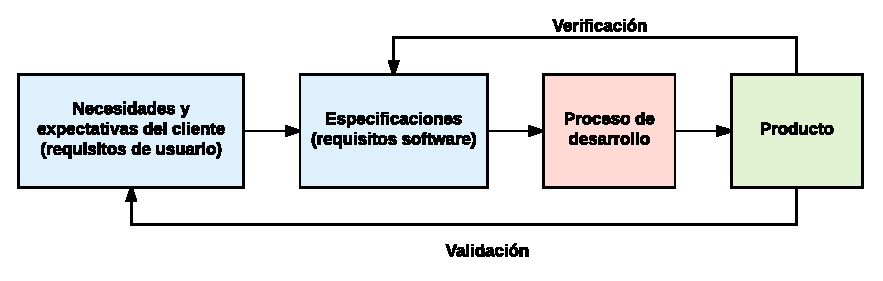
\includegraphics[width=12cm]{figures/verificacion_validacion_diagrama}
 	\caption{Verificación y validación \gls{software}.}
	\label{fig:verification_validation}
\end{figure}

\vspace{1cm}

\textit{Verificación \Gls{software}} Es el proceso de evaluación de los productos de trabajo (no el producto final real) de una fase de desarrollo para determinar si cumplen con los requisitos especificados para esa fase (los requisitos de \gls{software}). \textit{Validación \gls{software}} es el proceso de evaluación del producto final al final del proceso de desarrollo para determinar si satisface los requisitos especificados por el usuario al inicio del proyecto \cite{verification}.

\subsection{Pruebas de verificación}

Con el fin de realizar las pruebas de verificación, hemos seguido un proceso dinámico durante la fase de desarrollo del \gls{software}. Con estas pruebas queríamos responder a la pregunta: \emph{``¿Estamos construyendo el producto correctamente?''}. La Tabla \ref{tab:verification_tests} proporciona la plantilla utilizada para los test de verificación. Es necesario tener en cuenta que el formato del atributo ID es VET-XX, donde XX indica el número de test de verificación.
\clearpage

\begin{center}
\begin{table*}[htb]
\centering
\caption{Plantilla de pruebas de verificación.}
\begin{tabular}{@{}p{2.5cm} p{9cm}@{}} 
\toprule
\textbf{ID} 					& Test ID. \\
\midrule
\textbf{Nombre} 				& Nombre del test. \\
\midrule
\textbf{Requisitos} 		& Requisitos de \gls{software} cumplidos con este test. \\
\midrule
\textbf{Descripción} 		& Descripción del test. \\
\midrule
\textbf{Precondiciones}		& Las condiciones que siempre deben ser verdad antes de realizar el test. \\
\midrule
\textbf{Procedimiento}			& Una secuencia fija, paso a paso, de las actividades realizadas por el test. \\
\midrule
\textbf{Postcondiciones} 		& Las condiciones que siempre deben ser verdaderas justo después de realizar el test. \\
\midrule
\textbf{Evaluación} 			& \textit{OK} o \textit{Error}. \\
\bottomrule
\end{tabular}
\label{tab:verification_tests}
\end{table*}
\end{center}

A continuación, se especifican las pruebas de verificación.

\begin{center}
\begin{table*}[htb]
\centering
\caption{Test de verificación VET-01.}
\begin{tabular}{@{}p{2.5cm} p{13cm}@{}} 
\toprule
\textbf{ID} 					& VET-01. \\
\midrule
\textbf{Nombre} 				& Plataforma. \\
\midrule
\textbf{Requisitos} 		& SR-NF-PL01, SR-NF-PL02\\
\midrule
\textbf{Descripción} 		& Verificar que el \gls{software} puede ser utilizado en los navegadores especificados en los requisitos. \\
\midrule
\textbf{Precondiciones}		& 1. Utilizar un computador con sistema operativo Ubuntu 16.04 / Windows 10 / MacOS 10.2.5 .\\
							& 2. .Tener instalados los navegadores Microsft Edge 30+, Mozilla Firefox 45+, Google Chrome 50+ o Safari 10+. \\
\midrule
\textbf{Procedimiento}			& 1. Abrir el \gls{software} en cualquiera de los navegadores web especificados. \\
							& 2. Generar \gls{microcodigo}.\\
							& 3. Generar memoria principal.\\
							& 4. Ejecutar simulación.\\
\midrule
\textbf{Postcondiciones} 		&  La simulación ha sido completada satisfactoriamente sin ningún error de ejecución debido a la plataforma .\\
\midrule
\textbf{Evaluación} 			& OK \\
\bottomrule
\end{tabular}
\label{tab:vet01}
\end{table*}
\end{center}

\begin{center}
\begin{table*}[htb]
\centering
\caption{Test de verificación VET-02.}
\begin{tabular}{@{}p{2.5cm} p{13cm}@{}} 
\toprule
\textbf{ID} 					& VET-02. \\
\midrule
\textbf{Nombre} 				& Ejecución local. \\
\midrule
\textbf{Requisitos} 		& SR-NF-PL03, SR-NF-PL04\\
\midrule
\textbf{Descripción} 		& Verificar que el \gls{software} es ejecutado en local sin la necesidad de conexión a internet. \\
\midrule
\textbf{Precondiciones}		& 1. No tener acceso a Internet.\\
											& 2. Tener el código fuente de la herramienta descargado en local.\\
\midrule
\textbf{Procedimiento}			& 1. Abrir el \gls{software} en cualquiera de los navegadores web especificados. \\
							& 2. Generar \gls{microcodigo}.\\
							& 3. Generar memoria principal.\\
							& 4. Ejecutar simulación.\\
\midrule
\textbf{Postcondiciones} 		&  La simulación ha sido completada satisfactoriamente sin ningún error de ejecución debido a la conexión de red.\\
\midrule
\textbf{Evaluación} 			& OK \\
\bottomrule
\end{tabular}
\label{tab:vet02}
\end{table*}
\end{center}

\begin{center}
\begin{table*}[htb]
\centering
\caption{Test de verificación VET-03.}
\begin{tabular}{@{}p{2.5cm} p{13cm}@{}} 
\toprule
\textbf{ID} 					& VET-03. \\
\midrule
\textbf{Nombre} 				& Lenguaje de programación \acrshort{html}5. \\
\midrule
\textbf{Requisitos} 		& SR-NF-PL05\\
\midrule
\textbf{Descripción} 		& Verificar que el \gls{software} ha sido desarrollando utilizando \acrshort{html}5. \\
\midrule
\textbf{Precondiciones}		& 1. Tener el código fuente de la herramienta descargado en local. \\
\midrule
\textbf{Procedimiento}		& 1. Comprobar el código de los archivos fuente del simulador.\\
\midrule
\textbf{Postcondiciones} 		&  El simulador ha sido desarrollado mediante el lenguaje de programación \acrshort{html}5.\\
\midrule
\textbf{Evaluación} 			& OK \\
\bottomrule
\end{tabular}
\label{tab:vet03}
\end{table*}
\end{center}

\begin{center}
\begin{table*}[htb]
\centering
\caption{Test de verificación VET-04.}
\begin{tabular}{@{}p{2.5cm} p{13cm}@{}} 
\toprule
\textbf{ID} 					& VET-04. \\
\midrule
\textbf{Nombre} 				& Interfaz de usuario. \\
\midrule
\textbf{Requisitos} 		& SR-NF-UI01\\
\midrule
\textbf{Descripción} 		& Verificar que la interfaz del simulador es compatible tanto con \acrshort{pc} como con plataformas móviles. \\
\midrule
\textbf{Precondiciones}		& 1. Disponer de un \acrshort{pc} y de un dispositivo móvil. \\
											& 2. Los dispositivos deben tener instalados los navegadores web especificados previamente. \\
\midrule
\textbf{Procedimiento}			& 1. Abrir el \gls{software} en cualquiera de los navegadores web especificados. \\
							& 2. Generar \gls{microcodigo}.\\
							& 3. Generar memoria principal.\\
							& 4. Ejecutar simulación.\\
\midrule
\textbf{Postcondiciones} 		&  La interfaz del simulador es compatible tanto como \acrshort{pc} como con dispositivos móviles, visualizándose correctamente en cualquier pantalla de la herramienta.\\
\midrule
\textbf{Evaluación} 			& OK \\
\bottomrule
\end{tabular}
\label{tab:vet04}
\end{table*}
\end{center}

\begin{center}
\begin{table*}[htb]
\centering
\caption{Test de verificación VET-05.}
\begin{tabular}{@{}p{2.5cm} p{13cm}@{}} 
\toprule
\textbf{ID} 					& VET-05. \\
\midrule
\textbf{Nombre} 				& Tiempo medio por ciclo de reloj. \\
\midrule
\textbf{Requisitos} 		& SR-NF-P01\\
\midrule
\textbf{Descripción} 		& Verificar que el tiempo medio por ciclo de reloj del simulador no supera 0,1 segundos. \\
\midrule
\textbf{Precondiciones}		& 1. Disponer de un dispositivo con una versión de navegador web igual o superior a los indicados anteriormente. \\
\midrule
\textbf{Procedimiento}			& 1. Abrir el \gls{software} en cualquiera de los navegadores web especificados. \\
							& 2. Generar \gls{microcodigo}.\\
							& 3. Generar memoria principal utilizando un código \gls{ensamblador} que utiliza cada una de las partes de la arquitectura del simulador.\\
							& 4. Ejecutar simulación midiendo el tiempo de ejecución.\\
\midrule
\textbf{Postcondiciones} 		&  El tiempo de ejecución medio por ciclo de reloj excede 0,1 segundos.\\
\midrule
\textbf{Evaluación} 			& OK \\
\bottomrule
\end{tabular}
\label{tab:vet05}
\end{table*}
\end{center}

\begin{center}
\begin{table*}[htb]
\centering
\caption{Test de verificación VET-06.}
\begin{tabular}{@{}p{2.5cm} p{13cm}@{}} 
\toprule
\textbf{ID} 					& VET-06. \\
\midrule
\textbf{Nombre} 				& Arquitectura del simulador. \\
\midrule
\textbf{Requisitos} 		& SR-F-F01, SR-F-02, SR-F-03\\
\midrule
\textbf{Descripción} 		& Verificar que el \gls{software} simula una arquitectura de 32 bits con unidad de control microprogramable (con secuenciamiento implícito, saltos a nivel de microdirección y microsaltos condicionales). \\
\midrule
\textbf{Precondiciones}		& 1. Tener el código fuente de la herramienta descargado en local. \\
											& 2. Disponer de un dispositivo con una versión de navegador web igual o superior a los indicados anteriormente. \\
\midrule
\textbf{Procedimiento}		& 1. Comprobar el código de los archivos fuente del simulador que contienen el modelo \gls{hardware} a simular (sim\_hw\_*.js).\\
											& 2. Generar \gls{microcodigo} que define instrucciones de acceso a memoria, operaciones con el banco de registros, uso de los buses de la arquitectura del simulador, saltos a nivel de microdirección y microsaltos condicionales.\\
											& 3. Generar memoria principal utilizando un código \gls{ensamblador} que utiliza cada una de las partes de la arquitectura del simulador y las instrucciones de prueba definidas.\\
							& 4. Verificar que los resultados obtenidos de la ejecución son los resultados teóricos esperados.\\
\midrule
\textbf{Postcondiciones} 		&  El modelo \gls{hardware} ha sido definido correctamente, obteniendo los resultados esperados tras la simulación.\\
\midrule
\textbf{Evaluación} 			& OK \\
\bottomrule
\end{tabular}
\label{tab:vet06}
\end{table*}
\end{center}

\begin{center}
\begin{table*}[htb]
\centering
\caption{Test de verificación VET-07.}
\begin{tabular}{@{}p{2.5cm} p{13cm}@{}} 
\toprule
\textbf{ID} 					& VET-07. \\
\midrule
\textbf{Nombre} 				& Definición de juego de instrucciones. \\
\midrule
\textbf{Requisitos} 		& SR-F-F04, SR-F-F05, SR-F-F09, SR-F-F10, SR-F-F11, SR-F-F15\\
\midrule
\textbf{Descripción} 		& Verificar que el \gls{software} permite la definición del juego de instrucciones en el formato utilizado en la asignatura Estructura de Computadores. \\
\midrule
\textbf{Precondiciones}		& 1. Disponer de un dispositivo con una versión de navegador web igual o superior a los indicados anteriormente. \\
											& 2. Disponer de un juego de instrucciones base en el formato utilizado en la asignatura Estructura de Computadores. \\
											& 3. Disponer de un código \gls{ensamblador} que utiliza el juego de instrucciones utilizado en la asignatura Estructura de Computadores. \\
\midrule
\textbf{Procedimiento}		& 1. Generar \gls{microcodigo} mediante el juego de instrucciones proporcionado.\\
											& 2. Generar memoria principal utilizando el código \gls{ensamblador} proporcionado.\\
											& 3. Ejecutar simulación.\\
											& 4. Verificar que los resultados obtenidos de la ejecución son los resultados teóricos esperados.\\
\midrule
\textbf{Postcondiciones} 		&  La memoria de control y la memoria principal han sido generadas correctamente, realizándose la simulación de forma satisfactoria.\\
\midrule
\textbf{Evaluación} 			& OK \\
\bottomrule
\end{tabular}
\label{tab:vet07}
\end{table*}
\end{center}

\begin{center}
\begin{table*}[htb]
\centering
\caption{Test de verificación VET-08.}
\begin{tabular}{@{}p{2.5cm} p{13cm}@{}} 
\toprule
\textbf{ID} 					& VET-08. \\
\midrule
\textbf{Nombre} 				& Importación y exportación. \\
\midrule
\textbf{Requisitos} 		& SR-F-F07, SR-F-F08, SR-F-F13, SR-F-F14\\
\midrule
\textbf{Descripción} 		& Verificar que el \gls{software} permite tanto la importación como la exportación de/a fichero del juego de instrucciones y del código \gls{ensamblador}. \\
\midrule
\textbf{Precondiciones}		& 1. Disponer de un dispositivo con una versión de navegador web igual o superior a los indicados anteriormente. \\
											& 2. Disponer de un juego de instrucciones base en el formato utilizado en la asignatura Estructura de Computadores en un fichero. \\
											& 3. Disponer de un código \gls{ensamblador} que utiliza el juego de instrucciones utilizado en la asignatura Estructura de Computadores en un fichero. \\
\midrule
\textbf{Procedimiento}		& 1. Importar juego de instrucciones mediante el fichero proporcionado.\\
											& 2. Generar \gls{microcodigo}.\\
											& 3. Exportar juego de instrucciones.\\
											& 4. Importar código \gls{ensamblador} mediante el fichero proporcionado.\\
											& 5. Generar memoria principal.\\
											& 6. Exportar código \gls{ensamblador}.\\
											& 7. Verificar que la memoria de control y la memoria principal han sido generadas correctamente.\\
											& 8. Verificar que los ficheros exportados han sido generados correctamente.\\
\midrule
\textbf{Postcondiciones} 		&  La memoria de control, la memoria principal y los dos ficheros exportados han sido generados correctamente.\\
\midrule
\textbf{Evaluación} 			& OK \\
\bottomrule
\end{tabular}
\label{tab:vet08}
\end{table*}
\end{center}

\begin{center}
\begin{table*}[htb]
\centering
\caption{Test de verificación VET-09.}
\begin{tabular}{@{}p{2.5cm} p{13cm}@{}} 
\toprule
\textbf{ID} 					& VET-09. \\
\midrule
\textbf{Nombre} 				& Edición de texto. \\
\midrule
\textbf{Requisitos} 		& SR-F-F06, SR-F-F12\\
\midrule
\textbf{Descripción} 		& Verificar que el \gls{software} permite la edición del juego de instrucciones y del código \gls{ensamblador}. \\
\midrule
\textbf{Precondiciones}		& 1. Disponer de un dispositivo con una versión de navegador web igual o superior a los indicados anteriormente. \\
\midrule
\textbf{Procedimiento}		& 1. Definir un juego de instrucciones mediante la herramienta.\\
											& 2. Generar \gls{microcodigo}.\\
											& 3. Definir código \gls{ensamblador} mediante la herramienta.\\
											& 4. Generar memoria principal.\\
\midrule
\textbf{Postcondiciones} 		&  La memoria de control, la memoria principal  han sido generadas correctamente, pudiéndose editar desde la herramienta.\\
\midrule
\textbf{Evaluación} 			& OK \\
\bottomrule
\end{tabular}
\label{tab:vet09}
\end{table*}
\end{center}

\begin{center}
\begin{table*}[htb]
\centering
\caption{Test de verificación VET-10.}
\begin{tabular}{@{}p{2.5cm} p{13cm}@{}} 
\toprule
\textbf{ID} 					& VET-10. \\
\midrule
\textbf{Nombre} 				& Tipos de simulaciones. \\
\midrule
\textbf{Requisitos} 		& SR-F-F16, SR-F-F17, SR-F-F18, SR-F-F22\\
\midrule
\textbf{Descripción} 		& Verificar que el \gls{software} permite los tres tipos de simulación: ciclo a ciclo de reloj, instrucción a instrucción y simulación completa. \\
\midrule
\textbf{Precondiciones}		& 1. Disponer de un dispositivo con una versión de navegador web igual o superior a los indicados anteriormente. \\
											& 2. Tener la memoria de control y la memoria principal de la herramienta generadas. \\
\midrule
\textbf{Procedimiento}		& 1. Realizar la simulación del código cargado microinstrucción a microinstrucción.\\
											& 2. Reiniciar la simulación.\\
											& 3. Realizar la simulación del código cargado instrucción a instrucción.\\
											& 4. Reiniciar la simulación.\\
											& 5. Realizar la simulación completa del código cargado. \\
\midrule
\textbf{Postcondiciones} 		&  Las simulaciones han sido realizadas correctamente, obteniéndose los resultados teóricos esperados en ellas.\\
\midrule
\textbf{Evaluación} 			& OK \\
\bottomrule
\end{tabular}
\label{tab:vet10}
\end{table*}
\end{center}

\begin{center}
\begin{table*}[htb]
\centering
\caption{Test de verificación VET-11.}
\begin{tabular}{@{}p{2.5cm} p{13cm}@{}} 
\toprule
\textbf{ID} 					& VET-11. \\
\midrule
\textbf{Nombre} 				& Velocidad de simulación. \\
\midrule
\textbf{Requisitos} 		& SR-F-F19\\
\midrule
\textbf{Descripción} 		& Verificar que el \gls{software} permite la configuración de la velocidad de simulación. \\
\midrule
\textbf{Precondiciones}		& 1. Disponer de un dispositivo con una versión de navegador web igual o superior a los indicados anteriormente. \\
											& 2. Tener la memoria de control y la memoria principal de la herramienta generadas. \\
\midrule
\textbf{Procedimiento}		& 1. Realizar la simulación completa del código cargado.\\
											& 2. Reiniciar la simulación.\\
											& 3. Modificar velocidad de simulación. \\
											& 4. Realizar la simulación completa del código cargado.\\
\midrule
\textbf{Postcondiciones} 		&  Las simulaciones han sido realizadas correctamente, obteniéndose diferentes tiempos en función de la velocidad de simulación establecida.\\
\midrule
\textbf{Evaluación} 			& OK \\
\bottomrule
\end{tabular}
\label{tab:vet11}
\end{table*}
\end{center}

\begin{center}
\begin{table*}[htb]
\centering
\caption{Test de verificación VET-12.}
\begin{tabular}{@{}p{2.5cm} p{13cm}@{}} 
\toprule
\textbf{ID} 					& VET-12. \\
\midrule
\textbf{Nombre} 				& Información de las simulaciones. \\
\midrule
\textbf{Requisitos} 		& SR-F-F20, SR-F-21, SR-F-22\\
\midrule
\textbf{Descripción} 		& Verificar que el \gls{software} muestra los esquemas de la \acrshort{cpu} y la Unidad de control, modificando el color de las señales activas y buses actualizados y muestra la información del estado de los registros. \\
\midrule
\textbf{Precondiciones}		& 1. Disponer de un dispositivo con una versión de navegador web igual o superior a los indicados anteriormente. \\
											& 2. Tener la memoria de control y la memoria principal de la herramienta generadas. \\
\midrule
\textbf{Procedimiento}		& 1. Realizar la simulación del código cargado ciclo a ciclo de reloj.\\
\midrule
\textbf{Postcondiciones} 		&  Las simulaciones han sido realizadas correctamente, cambiándose el color de las señales activas y buses de datos actualizados en cada ciclo de reloj y mostrándose la información de los registros.\\
\midrule
\textbf{Evaluación} 			& OK \\
\bottomrule
\end{tabular}
\label{tab:vet12}
\end{table*}
\end{center}

\clearpage



La matriz de trazabilidad de las pruebas de verificación (Tabla \ref{tab:verification_matrix}) determina que todos los requisitos de \gls{software} se han verificado durante la fase de desarrollo del proyecto.

\vspace{2cm}


\begin{table}[htb]
\ra{1.3}
  \centering
  \caption{Matriz de trazabilidad de pruebas de verificación.}
  \begin{tabular}{@{}L{3cm}C{0.7cm}C{0.7cm}C{0.7cm}C{0.7cm}C{0.7cm}C{0.7cm}C{0.7cm}C{0.7cm}C{0.7cm}C{0.7cm}C{0.7cm}C{0.7cm}@{}}
    \toprule
     \thead{Requisitos} & \rothead{VET-01} & \rothead{VET-02} & \rothead{VET-03} & \rothead{VET-04} & \rothead{VET-05} & \rothead{VET-06} & \rothead{VET-07} & \rothead{VET-08} & \rothead{VET-09} & \rothead{VET-10} & \rothead{VET-11} & \rothead{VET-12}\\
    \midrule
    SR-F-F01 & - & - & - & - & - & \ding{51} & - & - & - & - & - & - \\
    SR-F-F02 & - & - & - & - & - & \ding{51} & - & - & - & - & - & - \\
    SR-F-F03 & - & - & - & - & - & \ding{51} & - & - & - & - & - & - \\
    SR-F-F04 & - & - & - & - & - & - & \ding{51} & - & - & - & - & - \\
    SR-F-F05 & - & - & - & - & - & - & \ding{51} & - & - & - & - & - \\
    SR-F-F06 & - & - & - & - & - & - & - &  & \ding{51} & - & - & - \\
    SR-F-F07 & - & - & - & - & - & - & - & \ding{51} & - & - & - & - \\
    SR-F-F08 & - & - & - & - & - & - & - & \ding{51} & - & - & - & - \\
    SR-F-F09 & - & - & - & - & - & - & \ding{51} & - & - & - & - & - \\
    SR-F-F10 & - & - & - & - & - & - & \ding{51} & - & - & - & - & - \\
    SR-F-F11 & - & - & - & - & - & - & \ding{51} & - & - & - & - & - \\
    SR-F-F12 & - & - & - & - & - & - & - & - & \ding{51} & - & - & - \\
    SR-F-F13 & - & - & - & - & - & - & - & \ding{51} & - & - & - & - \\
    SR-F-F14 & - & - & - & - & - & - & - & \ding{51} & - & - & - & - \\
    SR-F-F15 & - & - & - & - & - & - & \ding{51} & - & - & - & - & - \\
     SR-F-F16 & - & - & - & - & - & - & - & - & - & \ding{51} & - & - \\
    SR-F-F17 & - & - & - & - & - & - & - & - & - & \ding{51} & - & - \\
    SR-F-F18 & - & - & - & - & - & - & - & - & - & \ding{51} & - & - \\
    SR-F-F19 & - & - & - & - & - & - & - & - & - & - & \ding{51} & - \\
    SR-F-F20 & - & - & - & - & - & - & - & - & - & - & - & \ding{51} \\
    SR-F-F21 & - & - & - & - & - & - & - & - & - & - & - & \ding{51} \\
    SR-F-F22 & - & - & - & - & - & - & - & - & - & \ding{51} & - & \ding{51} \\
    SR-NF-PL01 & \ding{51} & - & - & - & - & - & - & - & - & - & - & - \\
    SR-NF-PL02 & \ding{51} & - & - & - & - & - & - & - & - & - & - & - \\
    SR-NF-PL03 & - & \ding{51} & - & - & - & - & - & - & - & - & - & - \\
    SR-NF-PL04 & - & \ding{51} & - & - & - & - & - & - & - & - & - & - \\
    SR-NF-PL05 & - & - & \ding{51} & - & - & - & - & - & - & - & - & - \\
    SR-NF-UI01 & - & - & - & \ding{51} & - & - & - & - & - & - & - & - \\
    SR-NF-P01 & - & - & - & - & \ding{51} & - & - & - & - & - & - & - \\
    \bottomrule
\end{tabular}
\label{tab:verification_matrix}
\end{table}    

\clearpage

\subsection{Pruebas de validación}


Para realizar las pruebas de validación, hemos comprobado el \gls{software} final, comparándolo con las necesidades del usuario especificadas en el Capítulo \ref{ch:analysis} \textit{\nameref{ch:analysis}}). Con estas pruebas queremos responder a la pregunta: \emph{``¿Hemos construido el producto adecuado?''}. La Tabla \ref{tab:validation_tests} proporciona la plantilla utilizada para los test de validación. Es necesario tener en cuenta que el formato del atributo ID es VAT-XX, donde XX indica el número de test de validación.


\begin{center}
\begin{table*}[htb]
\centering
\caption{Plantilla para test de validación.}
\begin{tabular}{@{}p{2.5cm} p{9cm}@{}} 
\toprule
\textbf{ID} 					& Test ID. \\
\midrule
\textbf{Nombre} 				& Nombre del test. \\
\midrule
\textbf{Requisitos} 		& Requisitos del usuario cumplidos con esta prueba. \\
\midrule
\textbf{Test de verificación} 	& Pruebas de verificación que nos ayudan a validar esta prueba. \\
\midrule
\textbf{Descripción} 		& Descripción de la prueba. \\
\midrule
\textbf{Precondiciones}		& Las condiciones que siempre deben ser verdad antes de realizar la prueba. \\
\midrule
\textbf{Procedimiento}			& Una secuencia fija, paso a paso, de las actividades realizadas por la prueba. \\
\midrule
\textbf{Postcondiciones} 		& Las condiciones que siempre deben ser verdaderas justo después de realizar la prueba. \\
\midrule
\textbf{Evaluación} 			& \textit{OK} o \textit{Error}. \\
\bottomrule
\end{tabular}
\label{tab:validation_tests}
\end{table*}
\end{center}


A continuación, especificamos las pruebas de validación.

\begin{center}
\begin{table*}[htb]
\centering
\caption{Test de validación VAT-01.}
\begin{tabular}{@{}p{2.5cm} p{9cm}@{}} 
\toprule
\textbf{ID} 					& VAT-01. \\
\midrule
\textbf{Nombre} 				& Juego de instrucciones. \\
\midrule
\textbf{Requisitos} 		& UR-C02, UR-C03 \\
\midrule
\textbf{Descripción} 		& Validar que el \gls{software} permite la definición del juego de instrucciones en el formato utilizado en la asignatura Estructura de Computadores mediante la carga de un fichero y la edición desde la herramienta, generando la memoria de control asociada y permitiendo la exportación del juego de instrucciones a un fichero. \\
\midrule
\textbf{Precondiciones}		& 1. Disponer de un dispositivo con una versión de navegador web igual o superior a los indicados anteriormente. \\
											& 2. Disponer de un juego de instrucciones base en el formato utilizado en la asignatura Estructura de Computadores. \\
\midrule
\textbf{Procedimiento}		& 1. Importar juego de instrucciones desde fichero.\\
											& 2. Editar el juego de instrucciones desde la herramienta.\\
											& 3. Generar memoria de control utilizando el juego de instrucciones cargado.\\
											& 4. Exportar el juego de instrucciones cargado a fichero. \\
\midrule
\textbf{Postcondiciones} 		&  La memoria de control ha sido generada correctamente, permitiéndose la carga desde fichero, la edición desde la herramienta y la exportación del juego de instrucciones a fichero.\\
\midrule
\textbf{Evaluación} 			& OK \\
\bottomrule
\end{tabular}
\label{tab:vat-01}
\end{table*}
\end{center}


\begin{center}
\begin{table*}[htb]
\centering
\caption{Test de validación VAT-02.}
\begin{tabular}{@{}p{2.5cm} p{9cm}@{}} 
\toprule
\textbf{ID} 					& VAT-02. \\
\midrule
\textbf{Nombre} 				& Código \gls{ensamblador}. \\
\midrule
\textbf{Requisitos} 		& UR-C04, UR-C05 \\
\midrule
\textbf{Descripción} 		& Validar que el \gls{software} permite la definición del código \gls{ensamblador} en el formato utilizado en la asignatura Estructura de Computadores mediante la carga de un fichero y la edición desde la herramienta, generando la memoria principal asociada y permitiendo la exportación del código \gls{ensamblador} a un fichero. \\
\midrule
\textbf{Precondiciones}		& 1. Disponer de un dispositivo con una versión de navegador web igual o superior a los indicados anteriormente. \\
											& 2. Disponer de un juego de instrucciones base en el formato utilizado en la asignatura Estructura de Computadores cargado en el simulador. \\
											& 3. Disponer de un código \gls{ensamblador} base en el formato utilizado en la asignatura Estructura de Computadores. \\
\midrule
\textbf{Procedimiento}		& 1. Importar código \gls{ensamblador} desde fichero.\\
											& 2. Editar el código \gls{ensamblador} desde la herramienta.\\
											& 3. Generar memoria principal utilizando el código \gls{ensamblador} cargado.\\
											& 4. Exportar el código \gls{ensamblador} cargado a fichero. \\
\midrule
\textbf{Postcondiciones} 		&  La memoria principal ha sido generada correctamente, permitiéndose la carga desde fichero, la edición desde la herramienta y la exportación del código \gls{ensamblador} a fichero.\\
\midrule
\textbf{Evaluación} 			& OK \\
\bottomrule
\end{tabular}
\label{tab:vat-02}
\end{table*}
\end{center}

\begin{center}
\begin{table*}[htb]
\centering
\caption{Test de validación VAT-03.}
\begin{tabular}{@{}p{2.5cm} p{9cm}@{}} 
\toprule
\textbf{ID} 					& VAT-03. \\
\midrule
\textbf{Nombre} 				& Simulación del modelo \gls{hardware} propuesto. \\
\midrule
\textbf{Requisitos} 		& UR-C01 \\
\midrule
\textbf{Descripción} 		& Validar que el \gls{software} permite la simulación del modelo \gls{hardware} propuesto. \\
\midrule
\textbf{Precondiciones}		& 1. Disponer de un dispositivo con una versión de navegador web igual o superior a los indicados anteriormente. \\
											& 2. Disponer de un juego de instrucciones base en el formato utilizado en la asignatura Estructura de Computadores cargado en el simulador. \\
											& 3. Disponer de un código \gls{ensamblador} base en el formato utilizado en la asignatura Estructura de Computadores cargado en el simulador. \\
\midrule
\textbf{Procedimiento}		& 1. Comprobar el código de los archivos fuente del simulador que contienen el modelo \gls{hardware} a simular (sim\_hw\_*.js).\\
											& 2. Ejecutar la simulación del código \gls{ensamblador}.\\
\midrule
\textbf{Postcondiciones} 		&  El modelo \gls{hardware} definido se corresponde con el modelo propuesto, siendo el resultado de la simulación el resultado teórico esperado.\\
\midrule
\textbf{Evaluación} 			& OK \\
\bottomrule
\end{tabular}
\label{tab:vat-03}
\end{table*}
\end{center}

\begin{center}
\begin{table*}[htb]
\centering
\caption{Test de validación VAT-04.}
\begin{tabular}{@{}p{2.5cm} p{9cm}@{}} 
\toprule
\textbf{ID} 					& VAT-04. \\
\midrule
\textbf{Nombre} 				& Tipos de simulaciones. \\
\midrule
\textbf{Requisitos} 		& UR-C06\\
\midrule
\textbf{Descripción} 		& Verificar que el \gls{software} permite los tres tipos de simulación: ciclo a ciclo de reloj, instrucción a instrucción y simulación completa. \\
\midrule
\textbf{Precondiciones}		& 1. Disponer de un dispositivo con una versión de navegador web igual o superior a los indicados anteriormente. \\
											& 2. Tener la memoria de control y la memoria principal de la herramienta generadas. \\
\midrule
\textbf{Procedimiento}		& 1. Realizar la simulación del código cargado microinstrucción a microinstrucción.\\
											& 2. Reiniciar la simulación.\\
											& 3. Realizar la simulación del código cargado instrucción a instrucción.\\
											& 4. Reiniciar la simulación.\\
											& 5. Realizar la simulación completa del código cargado. \\
\midrule
\textbf{Postcondiciones} 		&  Las simulaciones han sido realizadas correctamente, obteniéndose los resultados teóricos esperados en ellas.\\
\midrule
\textbf{Evaluación} 			& OK \\
\bottomrule
\end{tabular}
\label{tab:vat-04}
\end{table*}
\end{center}

\begin{center}
\begin{table*}[htb]
\centering
\caption{Test de validación VAT-05.}
\begin{tabular}{@{}p{2.5cm} p{9cm}@{}} 
\toprule
\textbf{ID} 					& VAT-05. \\
\midrule
\textbf{Nombre} 				& Velocidad de simulación. \\
\midrule
\textbf{Requisitos} 		& UR-C07\\
\midrule
\textbf{Descripción} 		& Verificar que el \gls{software} permite la configuración de la velocidad de simulación. \\
\midrule
\textbf{Precondiciones}		& 1. Disponer de un dispositivo con una versión de navegador web igual o superior a los indicados anteriormente. \\
											& 2. Tener la memoria de control y la memoria principal de la herramienta generadas. \\
\midrule
\textbf{Procedimiento}		& 1. Realizar la simulación completa del código cargado.\\
											& 2. Reiniciar la simulación.\\
											& 3. Modificar velocidad de simulación. \\
											& 4. Realizar la simulación completa del código cargado.\\
\midrule
\textbf{Postcondiciones} 		&  Las simulaciones han sido realizadas correctamente, obteniéndose diferentes tiempos en función de la velocidad de simulación establecida.\\
\midrule
\textbf{Evaluación} 			& OK \\
\bottomrule
\end{tabular}
\label{tab:vat-05}
\end{table*}
\end{center}

\begin{center}
\begin{table*}[htb]
\centering
\caption{Test de validación VAT-06.}
\label{tab:vat-06}
\begin{tabular}{@{}p{2.5cm} p{9cm}@{}} 
\toprule
\textbf{ID} 					& VAT-06. \\
\midrule
\textbf{Nombre} 				& Información de las simulaciones. \\
\midrule
\textbf{Requisitos} 		& UR-C08, UR-C09\\
\midrule
\textbf{Descripción} 		& Verificar que el \gls{software} muestra los esquemas de la \acrshort{cpu} y la Unidad de control, modificando el color de las señales activas y buses actualizados y muestra la información del estado de los registros. \\
\midrule
\textbf{Precondiciones}		& 1. Disponer de un dispositivo con una versión de navegador web igual o superior a los indicados anteriormente. \\
											& 2. Tener la memoria de control y la memoria principal de la herramienta generadas. \\
\midrule
\textbf{Procedimiento}		& 1. Realizar la simulación del código cargado ciclo a ciclo de reloj.\\
\midrule
\textbf{Postcondiciones} 		&  Las simulaciones han sido realizadas correctamente, cambiándose el color de las señales activas y buses de datos actualizados en cada ciclo de reloj y mostrándose la información de los registros.\\
\midrule
\textbf{Evaluación} 			& OK \\
\bottomrule
\end{tabular}
\end{table*}
\end{center}

\begin{center}
\begin{table*}[htb]
\centering
\caption{Test de validación VAT-07.}
\begin{tabular}{@{}p{2.5cm} p{9cm}@{}} 
\toprule
\textbf{ID} 					& VAT-07. \\
\midrule
\textbf{Nombre} 				& Plataforma. \\
\midrule
\textbf{Requisitos} 		& UR-R01, UR-R02\\
\midrule
\textbf{Descripción} 		& Verificar que el \gls{software} puede ser utilizado en los navegadores especificados en los requisitos. \\
\midrule
\textbf{Precondiciones}		& 1. Utilizar un computador con sistema operativo Ubuntu 16.04 / Windows 10 / MacOS 10.2.5 .\\
							& 2. .Tener instalados los navegadores Microsft Edge 30+, Mozilla Firefox 45+, Google Chrome 50+ o Safari 10+. \\
\midrule
\textbf{Procedimiento}			& 1. Abrir el \gls{software} en cualquiera de los navegadores web especificados. \\
							& 2. Generar \gls{microcodigo}.\\
							& 3. Generar memoria principal.\\
							& 4. Ejecutar simulación.\\
\midrule
\textbf{Postcondiciones} 		&  La simulación ha sido completada satisfactoriamente sin ningún error de ejecución debido a la plataforma .\\
\midrule
\textbf{Evaluación} 			& OK \\
\bottomrule
\end{tabular}
\label{tab:vat-07}
\end{table*}
\end{center}

\begin{center}
\begin{table*}[htb]
\centering
\caption{Test de validación VAT-08.}
\begin{tabular}{@{}p{2.5cm} p{9cm}@{}} 
\toprule
\textbf{ID} 					& VAT-08. \\
\midrule
\textbf{Nombre} 				& Interfaz de usuario. \\
\midrule
\textbf{Requisitos} 		& UR-R03\\
\midrule
\textbf{Descripción} 		& Verificar que la interfaz del simulador es compatible tanto con \acrshort{pc} como con plataformas móviles. \\
\midrule
\textbf{Precondiciones}		& 1. Disponer de un \acrshort{pc} y de un dispositivo móvil. \\
											& 2. Los dispositivos deben tener instalados los navegadores web específicados previamente. \\
\midrule
\textbf{Procedimiento}			& 1. Abrir el \gls{software} en cualquiera de los navegadores web especificados. \\
							& 2. Generar \gls{microcodigo}.\\
							& 3. Generar memoria principal.\\
							& 4. Ejecutar simulación.\\
\midrule
\textbf{Postcondiciones} 		&  La interfaz del simulador es compatible tanto como \acrshort{pc} como con dispositivos móviles, visualizándose correctamente en cualquier pantalla de la herramienta.\\
\midrule
\textbf{Evaluación} 			& OK \\
\bottomrule
\end{tabular}
\label{tab:vat-08}
\end{table*}
\end{center}

\begin{center}
\begin{table*}[htb]
\centering
\caption{Test de validación VAT-09.}
\begin{tabular}{@{}p{2.5cm} p{9cm}@{}} 
\toprule
\textbf{ID} 					& VAT-09. \\
\midrule
\textbf{Nombre} 				& Tiempo medio por ciclo de reloj. \\
\midrule
\textbf{Requisitos} 		& UR-R04\\
\midrule
\textbf{Descripción} 		& Verificar que el tiempo medio por ciclo de reloj del simulador no supera 0,1 segundos. \\
\midrule
\textbf{Precondiciones}		& 1. Disponer de un dispositivo con una versión de navegador web igual o superior a los indicados anteriormente. \\
\midrule
\textbf{Procedimiento}			& 1. Abrir el \gls{software} en cualquiera de los navegadores web especificados. \\
							& 2. Generar \gls{microcodigo}.\\
							& 3. Generar memoria principal utilizando un código \gls{ensamblador} que utiliza cada una de las partes de la arquitectura del simulador.\\
							& 4. Ejecutar simulación midiendo el tiempo de ejecución.\\
\midrule
\textbf{Postcondiciones} 		&  El tiempo de ejecución medio por ciclo de reloj excede 0,1 segundos.\\
\midrule
\textbf{Evaluación} 			& OK \\
\bottomrule
\end{tabular}
\label{tab:vat-09}
\end{table*}
\end{center}

\begin{center}
\begin{table*}[htb]
\centering
\caption{Test de validación VAT-10.}
\begin{tabular}{@{}p{2.5cm} p{9cm}@{}} 
\toprule
\textbf{ID} 					& VAT-10. \\
\midrule
\textbf{Nombre} 				& Ejecución local. \\
\midrule
\textbf{Requisitos} 		& UR-R05, UR-R06\\
\midrule
\textbf{Descripción} 		& Verificar que el \gls{software} es ejecutado en local sin la necesidad de conexión a internet. \\
\midrule
\textbf{Precondiciones}		& 1. No tener acceso a Internet.\\
											& 2. Tener el código fuente de la herramienta descargado en local.\\
\midrule
\textbf{Procedimiento}			& 1. Abrir el \gls{software} en cualquiera de los navegadores web especificados. \\
							& 2. Generar \gls{microcodigo}.\\
							& 3. Generar memoria principal.\\
							& 4. Ejecutar simulación.\\
\midrule
\textbf{Postcondiciones} 		&  La simulación ha sido completada satisfactoriamente sin ningún error de ejecución debido a la conexión de red.\\
\midrule
\textbf{Evaluación} 			& OK \\
\bottomrule
\end{tabular}
\label{tab:vat-10}
\end{table*}
\end{center}

\begin{center}
\begin{table*}[htb]
\centering
\caption{Test de validación VAT-11.}
\begin{tabular}{@{}p{2.5cm} p{9cm}@{}} 
\toprule
\textbf{ID} 					& VAT-11. \\
\midrule
\textbf{Nombre} 				& Tecnologías de desarrollo. \\
\midrule
\textbf{Requisitos} 		& UR-R07\\
\midrule
\textbf{Descripción} 		& Verificar que el \gls{software} ha sido desarrollando utilizando \acrshort{html}5. \\
\midrule
\textbf{Precondiciones}		& 1. Tener el código fuente de la herramienta descargado en local. \\
\midrule
\textbf{Procedimiento}		& 1. Comprobar el código de los archivos fuente del simulador.\\
\midrule
\textbf{Postcondiciones} 		&  El simulador ha sido desarrollado mediante el lenguaje de programación \acrshort{html}5.\\
\midrule
\textbf{Evaluación} 			& OK \\
\bottomrule
\end{tabular}
\label{tab:vat-11}
\end{table*}
\end{center}

\clearpage

La matriz de trazabilidad de las pruebas de validación (Tabla \ref{tab:validation_matrix}) determina que todos los requisitos de usuario han sido validados con el producto final.

\vspace{2cm}

\begin{table}[htb]
\ra{1.3}
  \centering
  \caption{Matriz de trazabilidad de pruebas de validación.}
  \begin{tabular}{@{}L{3cm}C{0.7cm}C{0.7cm}C{0.7cm}C{0.7cm}C{0.7cm}C{0.7cm}C{0.7cm}C{0.7cm}C{0.7cm}C{0.7cm}C{0.7cm}@{}}
    \toprule
     \thead{Requisitos} & \rothead{VAT-01} & \rothead{VAT-02} & \rothead{VAT-03} & \rothead{VAT-04} & \rothead{VAT-05} & \rothead{VAT-06} & \rothead{VAT-07} & \rothead{VAT-08} & \rothead{VAT-09} & \rothead{VAT-10} & \rothead{VAT-11}\\
    \midrule
    UR-C01 & - & - & \ding{51} & - & - & - & - & - & - & - & - \\
    UR-C02 & \ding{51} & - & - & - & - & - & - & - & - & - & - \\
    UR-C03 & \ding{51} & - & - & - & - & - & - & - & - & - & - \\
    UR-C04 & - & \ding{51} & - & - & - & - & - & - & - & - & - \\
    UR-C05 & - & \ding{51} & - & - & - & - & - & - & - & - & - \\
    UR-C06 & - & - & - & \ding{51} & - & - & - & - & - & - & - \\
    UR-C07 & - & - & - & - & \ding{51} & - & - & - & - & - & - \\
    UR-C08 & - & - & - & - & - & \ding{51} & - & - & - & - & - \\
    UR-C09 & - & - & - & - & - & \ding{51} & - & - & - & - & - \\
    UR-R01 & - & - & - & - & - & - & \ding{51} & - & - & - & - \\
    UR-R02 & - & - & - & - & - & - & \ding{51} & - & - & - & - \\
    UR-R03 & - & - & - & - & - & - & - & \ding{51} & - & - & - \\
    UR-R04 & - & - & - & - & - & - & - & - & \ding{51} & - & - \\
    UR-R05 & - & - & - & - & - & - & - & - & - & \ding{51} & - \\
    UR-R06 & - & - & - & - & - & - & - & - & - & \ding{51} & - \\
    UR-R07 & - & - & - & - & - & - & - & - & - & - & \ding{51} \\
    \bottomrule
\end{tabular}
\label{tab:validation_matrix}
\end{table}    

\lhead[\thepage]{CHAPTER \thechapter. PLANNING AND BUDGET}
\chead[]{}
\rhead[A Complete Simulator for Volunteer Computing Environments\leftmark]{\thepage}
\renewcommand{\headrulewidth}{0.5pt}

\lfoot[]{}
\cfoot[]{}
\rfoot[]{}
\renewcommand{\footrulewidth}{0pt}

%% This is an example first chapter.  You should put chapter/appendix that you
%% write into a separate file, and add a line \include{yourfilename} to
%% main.tex, where `yourfilename.tex' is the name of the chapter/appendix file.
%% You can process specific files by typing their names in at the 
%% \files=
%% prompt when you run the file main.tex through LaTeX.
\chapter{Planificación y presupuesto}
\label{ch:planning_and_budget}
\markboth{}{PLANNING AND BUDGET}

This chapter presents a detailed planning of the project (Section \ref{sec:planning}, \textit{\nameref{sec:planning}}). Then, we explain the project costs (Section \ref{sec:budget}, \textit{\nameref{sec:budget}}). At the end of the chapter, we comment on the socio-economic environment of the project ({Section \ref{sec:socioeconomic_environment}, \textit{\nameref{sec:socioeconomic_environment}}}).

\section{Planificación}
\label{sec:planning}

This section includes the complete project planning. First, we describe the software development methodology used. After that, we detail the time duration of each phase of the project, collecting all times in a Gantt chart.

\subsection{Justificación de la Metodología}

Due to its characteristics, we have divided our project into three iterations:

\begin{itemize}

\item \textbf{Basic functionality:} the first iteration has been to achieve the simulation of a simple distributed computing system. The aim of this phase has been to simulate client machines that exchange messages with a server through the a network.

\item \textbf{Client side:} this phase has been to incorporate all the necessary functionality on the client side (described in Chapter \ref{ch:design}, \textit{\nameref{ch:design}}).

\item \textbf{Server side:} this phase has been to incorporate all the necessary functionality on the server side (described in Chapter \ref{ch:design}, \textit{\nameref{ch:design}}).

\end{itemize}

It was necessary to have an iterative methodology used to develop each of the phases independently to join all together in the last stage and obtain the final product. For this purpose, we have analyzed three different software development methodologies: Software prototyping \cite{grimm1998}, the Waterfall model \cite{hebert1983} and the Spiral model \cite{boehm1988}. Software prototyping did not fit well because it requires building a prototype of the software in a short time. The Waterfall model is a sequential design process, used in software development processes, in which progress is seen as flowing steadily downwards (like a waterfall) through different phases. The problem with this methodology is that it does not allow iterations within the software development. Finally, the Spiral model allowed fragmenting the project into different iterations. The model combines the strengths of the other two models (simplicity and flexibility), and uses an iterative process. Although this model is slower than the other two, it allowed us to apply different iterations so we decided to apply it to the whole process.

\subsection{Ciclo de Vida}

The life cycle development process of the project has followed the Spiral lifecycle model \cite{boehm1988}. Figure \ref{fig:spiral_model} shows the Spiral model using a scheme.

\begin{figure}[htbp]
 	\centering
 	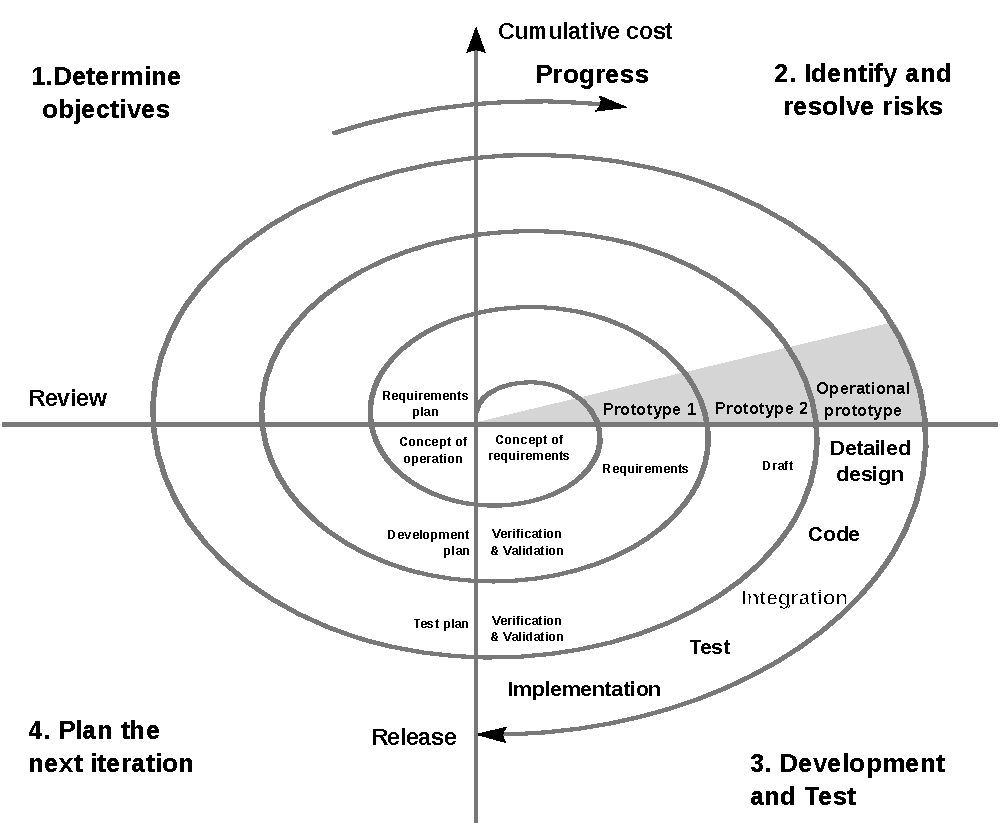
\includegraphics[width=12cm]{figures/spiral_model}
 	\caption{Spiral model (Boehm, 2000).}
	\label{fig:spiral_model}
\end{figure}

The Spiral model has four phases, which are repeated during the different iterations of the model. These phases are:

\begin{itemize}

\item \textbf{Planning} (Determine objectives in Figure \ref{fig:spiral_model}): the user requirements are gathered, a feasibility study of the system is performed, and the iteration objectives are determined. 

\item \textbf{Analysis} (Identify and resolve risks in Figure \ref{fig:spiral_model}): a full analysis of requirements is done and the potential risks are identified. This phase ends with a basic design.

\item \textbf{Development and Test}: Code implementation is done. Test cases and test results are performed.

\item \textbf{Evaluation} (Plan the next iteration in Figure \ref{fig:spiral_model}): Customers evaluate the software and provide their feedback. In this case, the student tries to get the supervisor's approval. This is  the \textit{critical task} of the life cycle, since we can only move on to the next iteration of the Spiral lifecycle model if this task is approved.

\end{itemize}

Each phase starts with a design goal and ends with the customer (the supervisor) reviewing the progress so far. As previously explained, we have divided the software development into three iterations: basic functionality, client side, and server side. In the last iteration, the complete software must undergo extensive testing in order to validate the simulator.


\subsection{Tiempo Estimado}

The Gantt chart (Figure \ref{fig:gantt}) shows all the tasks carried out during the project development. This project has been developed within a Collaboration in University Departments Scholarship \cite{colaboracion}, funded by the Spanish Ministry of Education, Culture, and Sport. The project began on November 2st, 2015, and ended on June 22, 2016, making a total of almost eight months of work. During this time, I have worked from Monday to Friday, four hours a day.

The Gantt chart shows all the tasks performed in each iteration of the spiral lifecycle model. Recall that the three iterations were: Basic functionality, Client side and Server side. In addition to the tasks (phases) mentioned above (Planning, Analysis, Development and Test, and Evaluation), we have included the Documentation task at the end of each iteration. The Documentation task has consisted mainly in drafting this bachelor thesis.


\begin{figure}[htbp]
 	\centering
 	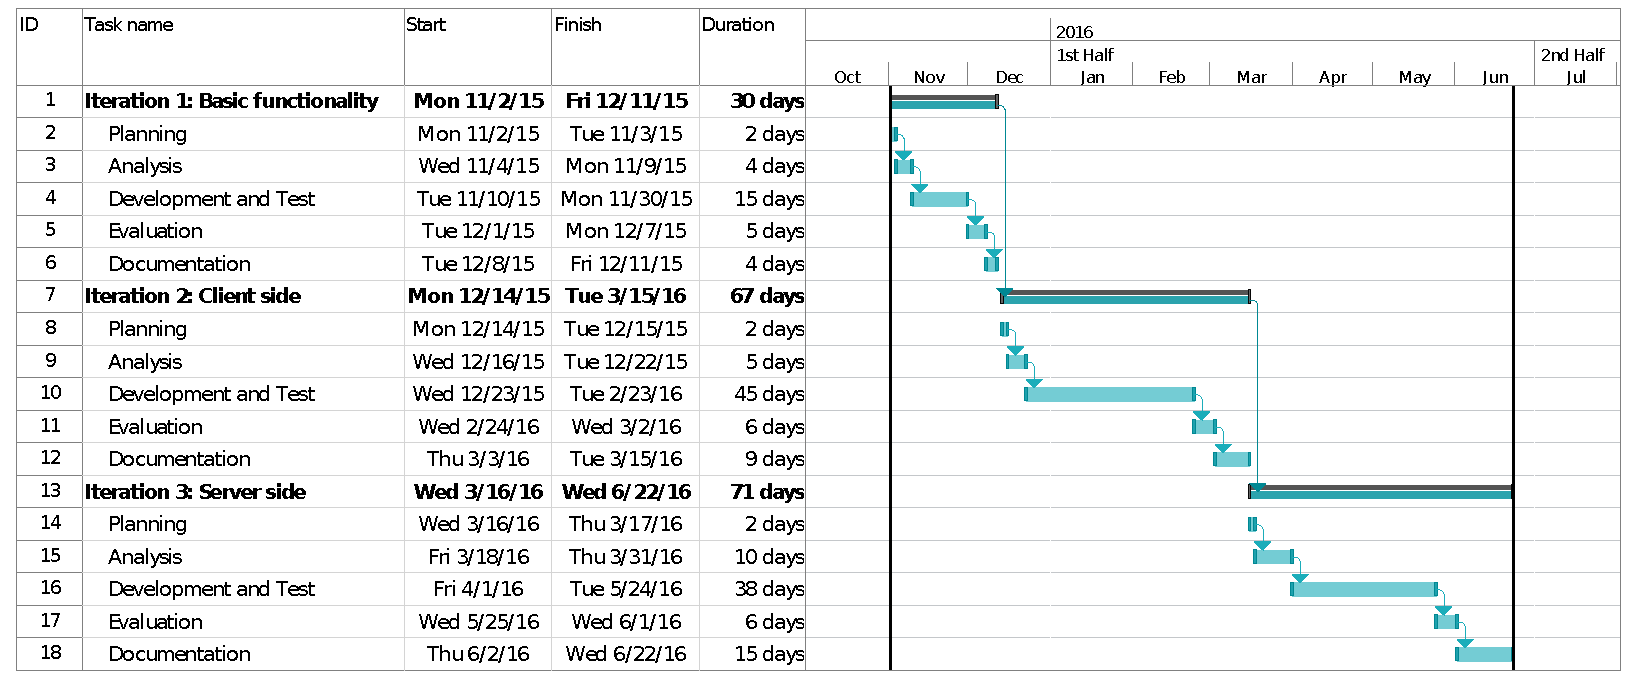
\includegraphics[width=16.5cm]{figures/gantt}
 	\caption{Gantt chart.}
	\label{fig:gantt}
\end{figure}

\section{Presupuesto}
\label{sec:budget}

This section details the overall project budget. On the one hand, we present the project costs and, on the other hand, we disclose the offer presented to the customer.

\subsection{Coste del Proyecto}

Table \ref{tab:project_information} summarizes the main features of the project including the total budget. 

\begin{center}
\ra{1.2}
\begin{table*}[htbp]
\centering
\begin{tabular}{@{}p{3.5cm} p{9cm}@{}} 
\toprule
\multicolumn{2}{c}{\textbf{\textit{Project Information}}}\\
\midrule
\textbf{Title} 					& A Complete Simulator for Volunteer Computing Environments \\
\midrule
\textbf{Author} 					& Saúl Alonso Monsalve \\
\midrule
\textbf{Department} 				& Computer Science and Engineering Department \\
\midrule
\textbf{Start date}				& 2nd of November of 2015 \\
\midrule
\textbf{End date}				& 22nd of June of 2016 \\
\midrule
\textbf{Duration} 				& 8 months \\
\midrule
\textbf{Indirect costs ratio} 	& 20 \% \\
\midrule
\textbf{Total budget} 			& 30,526.49 \\
\bottomrule
\end{tabular}
\caption{Project Information.}
\label{tab:project_information}
\end{table*}
\end{center}

Then the total budget of the project is broken down below.

\subsubsection{Costes Directos}

In this part, the direct costs of the project are presented. Table \ref{tab:dhrc} shows the direct costs caused by personnel costs, based on the planning presented in the previous section. The supervisor and the student have played the following roles:

\begin{itemize}

\item \textbf{Supervisor:} Project manager.

\item \textbf{Student:} Analyst, Developer, Tester.

\end{itemize} 

\begin{center}
\ra{1.2}
\begin{table*}[htbp]
\centering
\begin{tabular}{@{}p{3cm} R{3.5cm} R{2.2cm} R{2.4cm}@{}} 
\toprule
\textbf{Category} & \textbf{Cost per hour (\euro)} & \textbf{Hours} & \textbf{Total (\euro)} \\
\midrule
Project manager					& 60 						& 56			& 3,360 \\
Analyst			 				& 35							& 188		& 6,580 \\
Developer		 				& 35							& 316		& 11,060 \\
Tester		 					& 25							& 112		& 2,800 \\
\midrule
\textbf{\textit{Total}}			&							&			& \textbf{23,800.00}\\
\bottomrule
\end{tabular}
\caption{Human resources costs.}
\label{tab:dhrc}
\end{table*}
\end{center}

Table \ref{tab:dec} shows the direct costs caused by equipment acquisition and usage. The chargeable cost, C, is calculated using the following formula:

\begin{equation}
  C = \frac{d \cdot c \cdot u}{D}
\label{eq:costs}
\end{equation}

Where:

\begin{itemize}

\item \textbf{C:} Chargeable cost. It is equivalent to the depreciated value.

\item \textbf{d:} Time the equipment has been used.

\item \textbf{c:} Equipment cost. 

\item \textbf{u:} Project dedication. Percentage of time the equipment has been used.

\item \textbf{D:} Equipment depreciation period.

\end{itemize}

\begin{center}
\ra{1.2}
\begin{table*}[htbp]
\centering
\begin{tabular}{@{}p{2.5cm} C{1.8cm} C{2.1cm} C{2.1cm} C{2.7cm} C{2.3cm}@{}} 
\toprule
\textbf{Concept} & \textbf{Cost, c (\euro)} & \textbf{Dedication, u (\%)} & \textbf{Dedication, d (months)} & \textbf{Depreciation, D (months)} & \textbf{Chargeable cost, C (\euro)}\\
\midrule
Desktop \acrshort{pc}		 			& \multicolumn{1}{r}{799.99}		& \multicolumn{1}{r}{100}		& \multicolumn{1}{r}{8} 		& 	\multicolumn{1}{r}{36}	& 	\multicolumn{1}{r}{177.78} \\
Laptop 						& \multicolumn{1}{r}{529.99} 	& \multicolumn{1}{r}{25}			& \multicolumn{1}{r}{8} 		& 	\multicolumn{1}{r}{36}	& 	\multicolumn{1}{r}{29.44} \\
\acrshort{arcos} Tucan					& \multicolumn{1}{r}{89,501.60}	& \multicolumn{1}{r}{10}			& \multicolumn{1}{r}{6} 		& 	\multicolumn{1}{r}{60}	& 	\multicolumn{1}{r}{895.02} \\
\acrshort{arcos} Mirlo					& \multicolumn{1}{r}{2,469.99}	& \multicolumn{1}{r}{70}			& \multicolumn{1}{r}{6} 		& 	\multicolumn{1}{r}{60}	& 	\multicolumn{1}{r}{172.90} \\
Printer						& \multicolumn{1}{r}{399.24}		& \multicolumn{1}{r}{5}			& \multicolumn{1}{r}{3}		& 	\multicolumn{1}{r}{60}	& 	\multicolumn{1}{r}{1.00} \\
\midrule
\textbf{\textit{Total}}		&			&			& 			& &  \multicolumn{1}{r}{\textbf{1,276.14}}\\
\bottomrule
\end{tabular}
\caption{Equipment costs.}
\label{tab:dec}
\end{table*}
\end{center}

Furthermore, the equipment presented in Table \ref{tab:dec} is detailed below:

\begin{itemize}

\item \textbf{Desktop \acrshort{pc}:} All in One - Asus Z220ICUK, 21.5'', i5-6400T, 8GB, 1TB)		

\item \textbf{Laptop:} Toshiba L50D-C-19D, A10-8700P, 8GB \gls{ram} and 1TB.

\item \textbf{\acrshort{arcos} Tucan:} Cluster used by the research group \acrshort{arcos}.

\item \textbf{\acrshort{arcos} Mirlo:} Server used by the research group \acrshort{arcos}. 32GB \gls{ram} and eight i7 processors of 2.67GHz each.

\item \textbf{Printer:} HP LaserJet Enterprise P3015.

\end{itemize}

Other direct costs are shown in Table \ref{tab:odc}. These costs consist of office material, a toner for the printer, and the monthly travel pass. Office material includes: pencils, pens, notebooks, paper, tipex, and markers.

\begin{center}
\ra{1.2}
\begin{table*}[htbp]
\centering
\begin{tabular}{@{}p{5cm} R{3.5cm}@{}} 
\toprule
\textbf{Concept} & \textbf{Cost (\euro)} \\
\midrule
Office material					& 112.98				\\
Toner (x1) 			 			& 89.62				\\
Monthly travel pass (x8) 		& 160				\\
\midrule
\textbf{\textit{Total}}			& \textbf{362.60} 	\\
\bottomrule
\end{tabular}
\caption{Other direct costs.}
\label{tab:odc}
\end{table*}
\end{center}

\subsubsection{Resumen de Costes}

Table \ref{tab:cs} shows the complete summary of the project costs. Indirect costs (20\% of direct costs) consist of the electricity and water bills, telephone, Internet access, etc.

\begin{center}
\ra{1.2}
\begin{table*}[htbp]
\centering
\begin{tabular}{@{}p{5cm} R{5cm}@{}} 
\toprule
\multicolumn{2}{c}{\textbf{\textit{Costs summary}}}\\
\midrule
\textbf{Human resources} 				& 23,800.00 \\
\textbf{Equipment} 						& 1,276.14 \\
\textbf{Other direct costs} 				& 362.60 \\
\textbf{Indirect costs}					& 5,087.75 \\
\midrule
\textbf{\textit{Total budget}}			& \textbf{30,526.49} \\
\bottomrule
\end{tabular}
\caption{Costs summary.}
\label{tab:cs}
\end{table*}
\end{center}

The total budget for this project amounts to \textbf{30,526.49 \euro \ (thirty thousand five hundred twenty-six euro and forty-nine cent)}.

\subsection{Oferta de Proyecto Propuesta}

Table \ref{tab:offer} shows a detailed offer proposal. This offer includes the estimated risks (20\%), the expected benefits (15\%), and the Value Added Tax (Spanish \gls{iva}), which corresponds to 21\% \cite{iva2012}. After applying all theses concepts, the final amount for this project in case of sale to a third-party client is \textbf{50,973.14 \euro \ (fifty thousand nine hundred seventy-three euro and fourteen cent).}

\begin{center}
\ra{1.2}
\begin{table*}[htbp]
\centering
\begin{tabular}{@{}p{2.5cm} R{2.6cm} R{3.1cm} R{3.5cm}@{}} 
\toprule
\multicolumn{4}{c}{\textbf{\textit{Offer proposal}}}\\
\midrule
\textbf{Concept} & \textbf{Increment (\%)} & \textbf{Partial value (\euro)} & \textbf{Aggregated cost (\euro)} \\
\midrule
Project costs				& - 			& 30,526.49		& 30,526.49 \\
Risk			 				& 20			& 6,105.30		& 36,631.79 \\
Benefits		 				& 15			& 5,494.77		& 42,126.56 \\
IVA		 					& 21			& 8,846.58		& 50,973.14 \\
\midrule
\textbf{\textit{Total}}		&			&			& \textbf{50,973.14}\\
\bottomrule
\end{tabular}
\caption{Offer proposal.}
\label{tab:offer}
\end{table*}
\end{center}

\section{Entorno Socio-Económico}
\label{sec:socioeconomic_environment}

As commented in previous chapters, \gls{comsimboinc} can guide the design of \gls{boinc} projects. This means that \gls{boinc} project designers can perform accurate simulations using \gls{comsimboinc} before deploying the system. Thanks to this, designers can save money and resources, because they will know the performance of the system before deploying it. In addition, it can also save energy because designers will not need to perform tests using the original infrastructure, as they will only need to use \gls{comsimboinc} in order to analyze the functioning of different alternatives.

Moreover, \gls{boinc} operates as a platform for distributed applications in areas as diverse as mathematics, medicine, molecular biology, climatology, environmental science, and astrophysics. On the one hand, there are projects that help the scientific community, such as the SETI@home project \cite{Anderson2002SETI@home}, of which the purpose is to analyze radio signals, searching for signs of extraterrestrial intelligence; or the Citizen Science Grid project \cite{csgproject}, which is dedicated to supporting a wide range of research and educational projects. On the other hand, there are projects dedicated to the environmental care, such as the Climateprediction.net project \cite{climateprediction}, which studies climate. Therefore, our simulator indirectly contributes to both science and the environment.



\lhead[\thepage]{CAPÍTULO \thechapter. CONCLUSIONES Y TRABAJOS FUTUROS}
\chead[]{}
\rhead[WepSIM: Simulador de un procesador elemental con unidad de control microprogramada\leftmark]{\thepage}
\renewcommand{\headrulewidth}{0.5pt}

\lfoot[]{}
\cfoot[]{}
\rfoot[]{}
\renewcommand{\footrulewidth}{0pt}

%% This is an example first chapter.  You should put chapter/appendix that you
%% write into a separate file, and add a line \include{yourfilename} to
%% main.tex, where `yourfilename.tex' is the name of the chapter/appendix file.
%% You can process specific files by typing their names in at the 
%% \files=
%% prompt when you run the file main.tex through LaTeX.
\chapter{Conclusiones y trabajos futuros}
\label{ch:conclusions_and_future_work}
\markboth{}{CONCLUSIONS AND FUTURE WORK}

En este Capítulo presentamos las conclusiones del trabajo, revisamos los objetivos establecidos al principio de este documento, e incluimos algunas conclusiones personales. Además, discutiremos las principales contribuciones de nuestro trabajo, indicando también las publicaciones resultantes de este trabajo. Finalmente, discutimos el trabajo futuro.

\section{Conclusiones}

En este trabajo se ha descrito el diseño de WepSIM, un simulador de un procesador elemental con unidad de control microprogramada. Este trabajo presenta un nuevo simulador que resulta intuitivo, portable y extensible, sirviendo como complemento docente para la docencia en Estructura de Computadores. Este simulador, permite definir diferentes juegos de instrucciones y ejecutar y depurar código fuente que use el conjunto de instrucciones definido. También permite definir el comportamiento del procesador mediante microprogramación.

WepSIM, permite a los estudiante entender el funcionamiento de un procesador elemental de una forma sencilla, pudiendo ser usado desde un dispositivo móvil o un ordenador con un navegador Web moderno, sin la necesidad de ser instalado. De esta forma, los estudiantes pueden interactuar con el simulador aprendiendo y comprendiendo el funcionamiento del procesador elemental WepSIM, incluyendo los mecanismos de interacción con el software de sistema e integrando en una misma herramienta tanto la microprogramación como la programación en ensamblador.

El objetivo principal de este proyecto era desarrollar un simulador, que a diferencia de los existentes, pudiera simular de forma completa el comportamiento de un procesador elemental permitiendo comprobar el estado de los componentes en cada ciclo de reloj, de manera que ayudáse a los estudiantes a comprender y asimilar de forma sencilla y visual el funcionamiento de un procesador.  También hemos cumplido con todos los demás objetivos presentados en la introducción del documento:

\begin{itemize}

\item Simular la ejecución de el juego de instrucciones especificado en un computador denominado WepSIM desde el punto de vista de la micropogramación y la programación en ensamblador.

\item Permitir la especificación de diferentes juegos de instrucciones.

\item Permitir unificar la microprogramación y la programación en ensamblador.

\item Permitir al usuario la visualización en cada ciclo de reloj del estado y comportamiento del computador simulado.

\end{itemize}

A nivel personal, este trabajo me ha ayudado a empezar en el mundo de la investigación científica. He logrado aplicar una gran cantidad de los conocimientos adquiridos a lo largo del grado. Además, he aprendido importantes técnicas de modelado de hardware, compilación y simulación, las cuáles tienen una gran utilidad y complejidad y me han servido parar profundizar aún más en los conocimientos adquiridos en el grado. Por todo ello, es muy satisfactorio ver el resultado final obtenido, puesto que he logrado superar todos los problemas que han surgido a lo largo del proyecto.

\subsection{Contribuciones}

El proyecto llevado a cabo durante este Trabajo Fin de Grado encaja con muchas de las asignaturas estudiadas en el Grado en Ingeniería Informática de la Universidad Carlos III de Madrid, destacando los siguientes temas en particular:

\begin{itemize}

\item \textbf{Tecnología de Computadores} (asignatura obligatoria, Primer curso) en donde se introducen los componentes hardware y la lógica binaria.

\item \textbf{Estructura de Computadores} (asignatura obligatoria, Segundo curso) en donde se introducen las bases de la estructura y funcionamiento de un computador.

\item \textbf{Teoría de Autómatas y Lenguajes Formales} (asignatura obligatoria, Segundo curso) en donde se introducen las bases acerca de los lenguajes y gramáticas formales.

\item \textbf{Sistemas Operativos} (asignatura obligatoria, Segundo curso) en donde se introducen las bases del funcionamiento del sistema operativo.

\item \textbf{Arquitectura de Computadores} (asignatura obligatoria, Tercer curso) en donde se introducen las bases de la arquitectura de un computador.

\item \textbf{Diseño de Sistemas Operativos} (asignatura obligatoria, Tercer curso) en donde se introducen las bases del diseño de los distintos módulos de un sistema operativo.

\item \textbf{Dirección de proyectos de desarrollo de software} (asignatura obligatoria, Tercer curso) en donde se introducen las bases para la dirección y gestión de un proyecto de desarrollo de software.

\end{itemize}

El proyecto llevado a cabo durante esta tesis de licenciatura encaja con muchas de las materias estudiadas en el Grado de Informática e Ingeniería de la Universidad Carlos III de Madrid, destacando los siguientes temas en particular:

\subsection{Publicaciones}

Este Trabajo Fin de Grado ha hecho una importante contribución al campo de la docencia en Estructura y Arquitectura de Computadores. Las principales contribuciones de este trabajo se han publicado en dos artículos:

\begin{itemize}

\item \textbf{A. Calderón, F. García-Carballeira, and J. Prieto}, “WepSIM: Simulador modular e interactivo de un procesador elemental para facilitar una visión integrada de la microprogramación y la programación en ensamblador”, \textit{Enseñanza y aprendizaje de ingeniería de computadores}, vol. 6, 35-53,2016. \cite{mateos2016wepsim}

\item \textbf{J. Prieto, A. Calderón, F. García-Carballeira, and S. Alonso-Monsalve}, “WepSIM: simulador integrado de microprogramación y programación en ensamblador”, \textit{Jornadas sarteco 2016}. \cite{arcos2032}

\end{itemize}

Además, en el momento de la entrega de este documento también otro artículo enviado a la espera de su aceptación.

\section{Trabajos Futuros}

Actualmente, hay varias líneas de trabajos futuros en las cuáles estamos trabajando.

\begin{itemize}

\item En cuanto a mejoras en el modelo hardware:

\begin{itemize}

\item Introducir más elementos hardware, como por ejemplo una caché, de forma que se amplíen los contenidos de la asignatura incluídos en la herramienta.

\item Introducir un modelo hardware basado en \textit{pipeline}, permitiendo el uso de la herramienta en aquellas asignaturas que utilizan este modelo de arquitectura. 

\end{itemize}

\item En cuanto a mejoras en el modelo software:

\begin{itemize}

\item Añadir revisión semántica del código, permitiendo identificar y notificar los errores de programación al usuario.

\item Añadir nuevos juegos de instrucciones a la herramienta como por ejemplo el ensamblador ARM, permitiendo la utilización de diferentes lenguajes en la herramienta.

\item Estudiar el ensamblador de MIPS/ARM generado con GCC/Clang de forma que pueda ser usado directamente en WepSIM.

\end{itemize}

\item En cuanto a mejoras en la herramienta:

\begin{itemize}

\item Añadir un módulo de corrección automática de prácticas a la herramienta, de forma que los estudiantes puedan practicar con ella y comprobar la validez de sus ejercicios.

\item Migrar la herramienta como aplicación móvil mediante el \emph{plugin} Apache Cordova, de forma que la herramienta no quede ligada al uso mediante navegador web.

\end{itemize}

\end{itemize}



\lhead[\thepage]{APÉNDICE A. SUMMARY}
\chead[]{}
\rhead[WepSIM: Simulador de un procesador elemental con unidad de control microprogramada]{\thepage}
\renewcommand{\headrulewidth}{0.5pt}

\lfoot[]{}
\cfoot[]{}
\rfoot[]{}
\renewcommand{\footrulewidth}{0pt}

\appendix
\clearpage
\addappheadtotoc
\appendixpage
\chapter{Summary}
\label{ch:apendicea}

\section*{Introduction}

Teaching the topics related to the architecture of a computer is a basic and fundamental part of the training of computer science students. In these subjects, students achieve a low-level vision and understanding of the components of a computer. In order to facilitate the correctly understanding of the theoretical foundations, it is necessary to use practical classes, where the student should interact with the architecture of a computer in a similar way to that one explained in theory and also manage to extrapolate the theoretical foundations to the actual behavior.

One of the main problems when preparing these practical classes is to emulate the necessary resources seen in the theoretical classes. Currently, there are different tools that enable the emulation of different components of a computer. However, there is a lack of tools that unify the simulation of these components, being a problem when trying to obtain a global view of the operation of a computer.

These tools can be classified into two main types: emulators and simulators. An emulator is a software that imitates the behavior of a computer, so that programs designed for a particular architecture can be executed in a different one. On the other hand, a simulator is a software that aims to reproduce the behavior of a computer, but with a lower level of realism than the emulators.

There are different simulators that can be used in order to work with the main aspects treated in the subjects of ``Computer Architecture and Computer Sctructure'' such as assembler, cache, etc. Most of these simulators are focused on a specific type of simulation, which implies that, to obtain a global vision on the architecture of the computer several simulators are needed. Therefore, it is much better to count with a tool that offers a complete simulation of the architecture and combines the maximum possible functionalities.

We identify another important problem: most of the simulators are designed for running as PC applications. One of the goals we put forward with WepSIM is that it could be used in smartphones or tablets in order to offer greater flexibility in its usage to the student.

In addition to having a portable simulator, it must also be as self-contained as possible. Therefore, it must integrate support for its use inside the tool(not as a separate document that serves as a user manual to be printed), allowing the end-user to make full use of the application without the need of getting out of it.

In conclusion, we have considered how to offer a simulator that is simple and modular, and that at the same time allows to integrate the teaching of the microprogramming language with programming in assembly. In particular, it can be used to microprogram a customized instruction set and observe the basic operation of a processor, as well as to create assembler programs based on the assembler defined by the above microcode. This is of great help, for example, for system programing, since it is possible to follow how the software interacts in assembly with the hardware in the treatment of interruptions. The idea is to offer a simulator that offers a global vision of a computer, integrating both hardware and software components and also avoiding the extra time involved in learning different tools.


\section*{Objectives}

The main objective of this project is to design and develop a simulator, which, unlike the existing ones, can fully simulate the behavior of an elementary processor allowing to check the state of the components in each clock cycle, so that it helps the students to understand and assimilate in a simple and visual way the operation of a processor. The secondary objectives, derived from the main objective, are as follow:

\begin{itemize}

\item \textbf{O1:} Simulate the execution of the set of instructions specified in a computer called WepSIM from the point of view of microprogramming and programming in assembly.

\item \textbf{O2:} Allow the specification of different and customized sets of instructions.

\item \textbf{O3:} Allow unified microprogramming in a computer and programming in assembly language.


\item \textbf{O4:} Allow the user to display in each clock cycle the status and behavior of the simulated computer.

\end{itemize}

\section*{WepSIM Elemental Processor}

WepSIM is an elementary processor with an integrated microprogrammed control unit designed by the staff of the research group ARCOS of the University Carlos III of Madrid. This processor design is used for teaching in the subject ``Computer Structure''.

In Figure \ref{fig:wepsimCPU_figure_summary}, the structure of the WepSIM Elemental Processor is shown. WepSIM consists of a memory module, a keyboard device, a display device, and a generic I/O device that can be used to work with interrupts.

\begin{figure}[htbp]
 	\centering
 	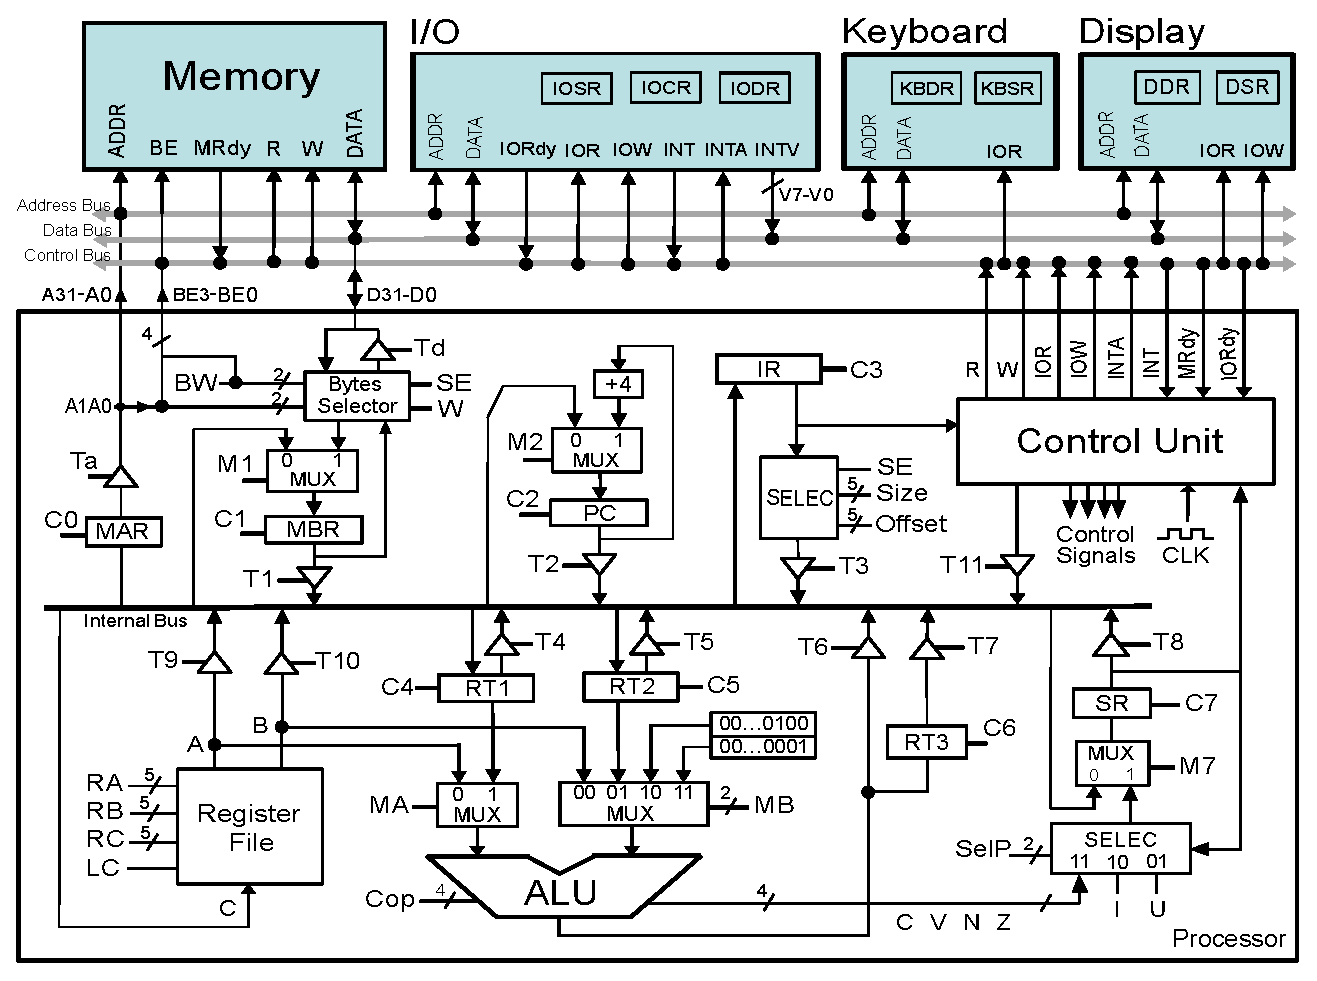
\includegraphics[width=11cm]{figures/processor6}
 	\caption{CPU Architecture WepSIM.}
	\label{fig:wepsimCPU_figure_summary}
\end{figure}

\begin{figure}[htbp]
 	\centering
 	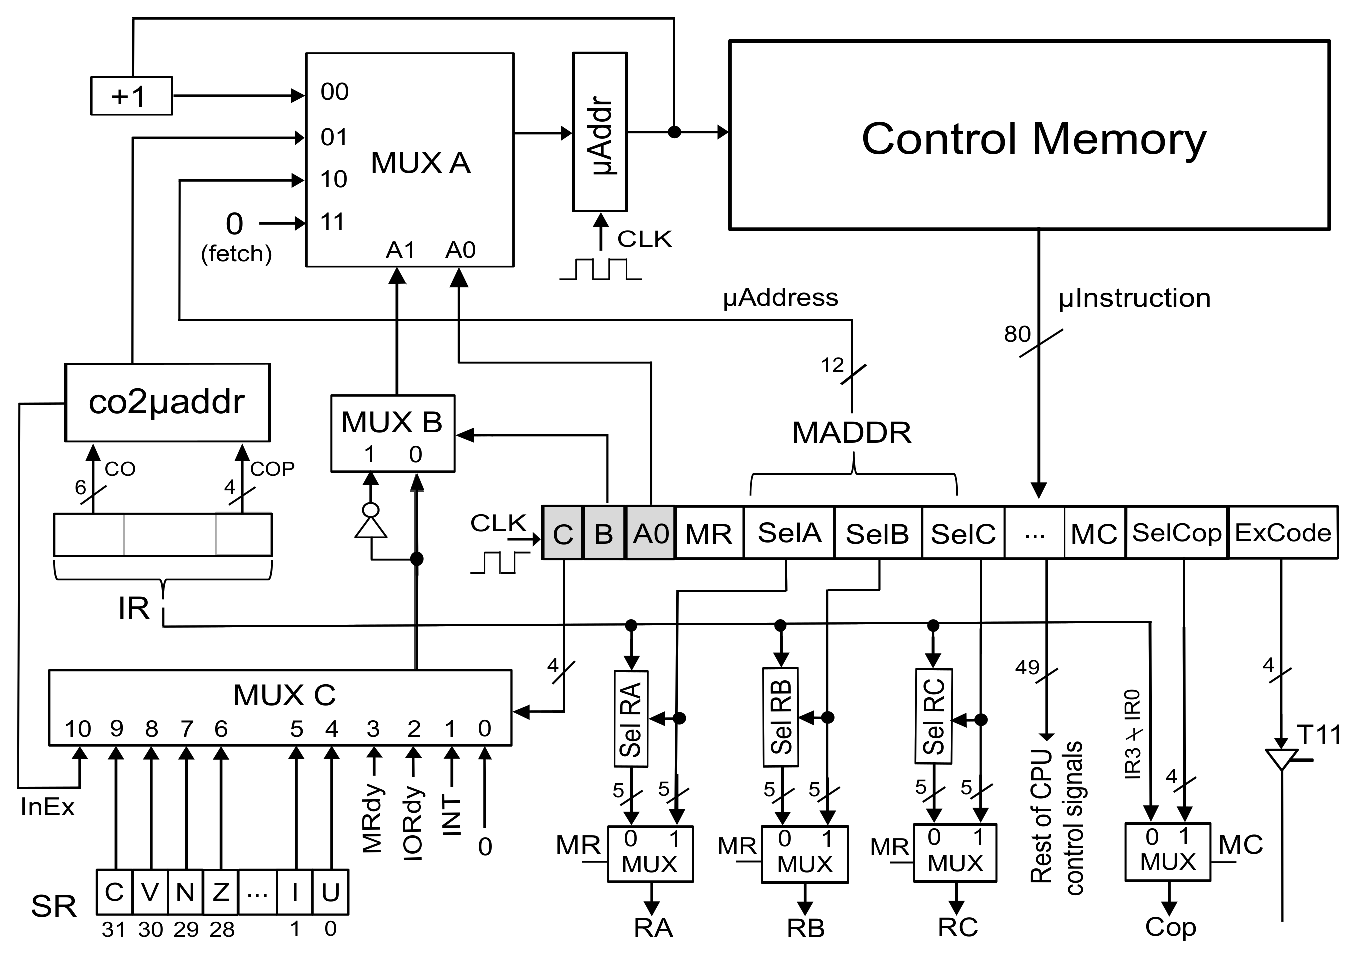
\includegraphics[width=11cm]{figures/controlunit6}
 	\caption{Control unit architecture in WepSIM.}
	\label{fig:wepsimCU_figure_summary}
\end{figure}


WepSIM incorporates a 32bit processor that includes a byte addressable memory,  a bank of 32 registers and two additional registers (\emph{RT1 and RT2}) that are not visible to the assembly programmer but allow temporary storage of data for the carrying out of intermediate operations. From the registers, it is possible to forward the values to operate in an \emph{ALU} that implements the 15 most common arithmetic-logic operations. The \emph{PC} registry has its own 4-add operator, so it is not necessary to make use of the \emph{ALU} for this operation. The result of the operations performed in the \emph{ALU} can be stored in a temporary register (\emph{RT3}) that is also invisible to the assembly programmer, or sent directly to the internal bus through the corresponding tristate.


The status register \emph{(SR)} can be updated with the resulting flags of the last operation of the \emph{ALU (O, N and Z)}. To do this, \emph{SELEC/SelP} represents a circuit block that allows indicating which part of the state register (\emph{SR}) must be updated. To the right of \emph{SELEC/SelP} the bits of the \emph{SR} status register enter (\emph{Input = ONZIU}) and \emph{SelP} allows to select which group of these bits will be updated in the status register: bits \emph{O, N and Z} with the values coming of the \emph{ALU}, the bit I with the indicated value or the bit \emph{U} with the indicated value for the same.

The instruction register (\emph{IR}) is associated with a selector module (higher level circuit than a multiplexer, etc.), which allows the selection of a segment of the binary value stored in the instruction register that will pass to \emph{T3}.

In particular, the position (offset, where 0 represents the least significant bit of the \emph{IR} register) and the number of bits (\emph{Size}) to be taken from that initial position is indicated, and wether if sign extension (\emph{SE}) is desired before passing the value to the \emph{T3} input.

The \emph{MAR} and \emph{MBR} registers are used to store the address and content associated with this address in read/write operations with memory. The memory is designed for synchronous or asynchronous operation. It currently works synchronously, but has the \emph{MRdy} signal for working asynchronously in the future. The selection circuit allows the user to indicate which portion of the memory word is the desired one (one byte, two bytes, or a complete four-byte word).

There are also three I / O devices: a keyboard, a display and a generic device that can be configured to generate various types of interrupts.

Finally, the Control Unit generates the control signals for each clock cycle. The Figure \ref{fig:wepsimCU_figure_summary} shows the Control Unit in more detail. It is a microprogrammed control unit with implicit sequencing. The control signals for the current clock cycle are stored in the micro-instruction register (the one with the fields \emph{A0, B, C, SelA}, etc.). The contents of this record come from the control memory, specifically from the content in the position to which the micro-address register points. The micro-address stored in this register can be modified using the ``MUX'' multiplexer. There are four options: the current micro-address plus one, a micro-address indicated in the micro-instruction itself (which overlaps with \emph{SelA, SelB} and partially with \emph{SelE}), the first micro-address associated with the operation code field of the instruction of the \emph{IR} register, and finally the value zero, which is the address of the control memory where the microprogram corresponding to the fetch is stored. The micro address can be selected conditionally by using the ``MUX C '' multiplexer that allows to select the status register bits (SR) or values of the I/O control signals. 

The \emph{SelRA, SelRB and SelRE} selector circuits are used to generate the values corresponding to the selector signals of the register bank \emph{RA, RB and RE}. These selectors take as input the 32 bits of the instruction register (\emph{IR}) on one side and the field \emph{SelA, SelB and SelE} on the other, so that they take \emph{SelX} as the displacement within the instruction register (from 0 to 32) from where Take the next 5 bits corresponding to the \emph{RA, RB or RE} signals. They thus allow to select 5 consecutive bits of the 32 bits of the instruction register.

The MR multiplexer is used to indicate whether the \emph{RA, RB and RE} signals are literally the values stored in \emph{SelA, SelB and SelE} (MR = 1) or if \emph{SelA, SelB and SelE} indicate the offset within the instruction where the values to be used for \emph{RA, RB and RE}. The latter allows the instruction to indicate the registers to be used as operands in the register bank, instead of indicating them from the micro-instruction.

For the \emph{Cop} signal (operation code in the \emph{ALU}), the \emph{MC} signal can be used to take the \emph{SelCop} value of the micro-instruction (\emph{MC} = 1) or the 4 least significant bits of the instruction register (MC = 0), ie \emph{IR3 -IR0}.

\section*{Simulator design}

In order for the teachers of the Computer Structure subject to use a tool that helps to explain the theoretical concepts of the subject, and that, at the same time, students can employ to understand the main concepts and to carry out the subject's practices later we propose the design and implementation of a web tool that realistically simulates an elementary processor with a microprogrammable control unit.

This simulator will be developed as a web tool due to the portability it provides, since it can be executed on a large number of different devices regardless of the operating system use, only needing a web browser for its correct operation. In this way, teachers and students will be able to use the tool without depending on their installation in the device to be used, even allowing the students to practice on mobile devices.

To achieve this portability, the simulator has been developed in HTML5 (HTML + JavaScript + CSS) making it possible to run on any platform (smartphones, tablets, PC, etc.) being compatible with Microsoft Edge, Mozilla Firefox, Google Chrome or Safari. In addition, the tool depends on the following frameworks or libraries: JQuery, JQueryUI, JQuery Mobile, Knockout, and BootStrap.

Therefore, the chosen solution is able to unify in a single tool all the features required for the teaching of Computer Structure with a high level of detail, with high availability by facilitating it as a web tool, and being portable, since it an be executed on a large number of different devices, always looking for a solution without the need for a server.

\subsection*{Simulator Architecture}

The architecture of the solution presented in this work consists of three main elements:

\begin{itemize}
\item \textbf{Hardware model:} allows the user to define the hardware to use.
\item \textbf{Software model:} allows the user to define the set of instructions to use.
\item \textbf{Simulation kernel:} simulates hardware operation by running the microcode / machine language previously defined.
\end{itemize}

The hardware model allows the user to define the typical elements of a computer (main memory, processor, etc.) in a modular way. The way in which these elements are defined balances two opposing objectives: it must be complete enough to imitate the main aspects of reality, but also minimal enough to facilitate its use. Above all, it is intended to be a didactic tool.

The software model allows defining the microcode and assembler based on this microcode as intuitively as possible. The assembly used is given by a set of instructions that can be defined by the user.These instructions try to be flexible enough to be able to define different types and sets of instructions, such as MIPS or ARM.

The third element of the proposed architecture is a kernel that takes as input the described hardware model and the working software model, and is responsible for showing the operation of the hardware with the given software.

\begin{figure}[htbp]
 	\centering
 	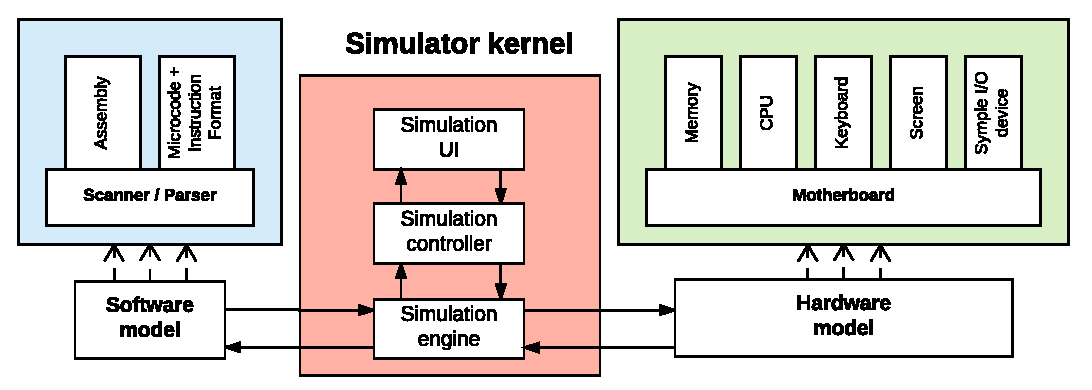
\includegraphics[width=14cm]{figures/architecture_diagram}
 	\caption{WepSIM Architecture.}
	\label{fig:architecture_diagram_summary}
\end{figure}

Figure \ref{fig:architecture_diagram_summary} summarizes the architecture of WepSIM. The starting point is the hardware model that describes the processor to be simulated. This includes the processor, memory, and some I/O devices such as keyboard, display, and a single I/O device that generates interrupts. The hardware model describes the overall state of the processor. From the processor's overall state, the simulation kernel updates the state in each clock cycle.

The simulated control unit stores the control signals of each cycle in a control memory. The control memory has all the microprograms for the instructions with which the processor works, and the fetch instruction to be able to read the instructions from the memory and to decode them.

The microcode (the contents of the control memory) together with the format of each instruction (fields of the instruction and its length) is described in a text file. The software model reads this file, translates it to binary and loads it into the processor. The definition of the assembly language to be used is described together with the microcode, and the software model allows to translate programs written in said assembler to binary.


The simulation kernel asks the subsystem of the software model for the defined microcode, the description of the instruction format and the contents of the main memory. The binaries are loaded into the elements of the hardware model, and then the simulation kernel updates the global state in each clock cycle.

WepSIM has a simulation controller that is responsible for updating the clock cycle and displaying the global status. The simulation interface subsystem updates the user interface. When the user uses the user interface to request an operation, the simulation interface subsystem moves the request to the simulation controller. In this way, a basic Model-View-Controller (MVC) design is used for the WepSIM architecture.

\section*{Conclusions and future work}

This section presents the conclusions obtained from the project, reviews the objectives set out at the beginning of this document, and includes some personal observations. In addition, we discuss the main contributions of our work, also indicating the publications resulting from this project. Finally, future work is discussed.

\section*{Conclusions}

In this work, we have described the design of WepSIM, an elementary processor simulator with a microprogrammed control unit. This work presents a new simulator that is intuitive, portable and extensible, serving as a teaching complement for teaching in Computer Structure. This simulator enables the definition of different sets of instructions and the execution and debugging of source code. It also allows to define the behavior of the processor by microprogramming instructions, also defined by the end-users.

WepSIM allows students to understand the operation of an elementary processor in a simple way, can be used from a mobile device or a computer with a modern Web browser without the need of being installed. In this way, students can interact with the simulator by learning and understanding the operation of the WepSIM elementary processor, including the mechanisms of interaction with the system software and integrating in the same tool both the microprogramming and the programming in assembler.

The main objective of this project was to develop a simulator, which, in contrast to existing ones, could completely simulate the behavior of an elementary processor, allowing to check the state of the components in each clock cycle, so that students understand and assimilate in a simple and visual way the operation of a processor. We have also met all the other objectives presented in the introduction of the document:

\begin{itemize}

\item \textbf{O1}, A tool has been designed that simulates the execution of the instruction set specified in a computer called WepSIM, from the point of view of microprogramming and assembly programming.

\item \textbf{O2}, The tool allows the specification of different instructions.

\item \textbf{O3}, The tool unifies the microprogramming of a computer and programming in assembly language.

\item \textbf{O4}, The tool allows the user to display in each clock cycle the state and behavior of the simulated computer.

\end{itemize}

On a personal level, this work has helped me to enter the world of scientific research. I have been able to apply a great deal of the knowledge acquired throughout the degree. In addition, I have learned important techniques of hardware modeling, compilation and simulation, which have a great utility and complexity and have served me to deepen even more in the knowledge acquired in the degree. For all this, it is very satisfying to see the final result obtained, since I have managed to overcome all the problems that have arisen throughout the project.

\subsection*{Contributions}

The project carried out during this Bachelor Thesis fits with many of the subjects studied in the Degree in Computer Engineering of the University Carlos III of Madrid, highlighting the following topics in particular:

\begin{itemize}

\item \textbf{Computer technology} (Compulsory subject, First course) Where the hardware components and binary logic are introduced.

\item \textbf{Computer structure} (Compulsory subject, Second course) Where the bases of the structure and operation of a computer are introduced.

\item \textbf{Formal languages and Automata theory} (Compulsory subject, Second course) Where the bases are introduced about the formal languages and grammars.

\item \textbf{Operating systems} (Compulsory subject, Second course) Where the bases of the operation of the operating system are introduced.

\item \textbf{Computer architecture} (Compulsory subject, Third course) Where the bases of the architecture of a computer are introduced.

\item \textbf{Operating systems design} (Compulsory subject, Third course) Where the bases of the design of the different modules of an operating system are introduced.

\item \textbf{Software development projects management} (Compulsory subject, Third course) Where the bases for the management and management of a software development project are introduced.

\end{itemize}

\subsection*{Publications}

This bachelor thesis has permitted to make an important contribution to the field of teaching in Structure and Computer Architecture. In addition, the following scientific articles have been published:

\begin{itemize}

\item \textbf{A. Calderón, F. García-Carballeira, and J. Prieto}, “WepSIM: Simulador modular e interactivo de un procesador elemental para facilitar una visión integrada de la microprogramación y la programación en ensamblador”, \textit{Enseñanza y aprendizaje de ingeniería de computadores}, vol. 6, 35-53,2016. \cite{mateos2016wepsim}

\item \textbf{J. Prieto, A. Calderón, F. García-Carballeira, and S. Alonso-Monsalve}, “WepSIM: simulador integrado de microprogramación y programación en ensamblador”, \textit{Jornadas sarteco 2016}. \cite{arcos2032}

\end{itemize}

In addition, at the time of delivery of this document, there is also another item sent waiting for its acceptance.

\clearpage

\section*{Future works}

Currently, there are many lines of future work in which we are working on:

\begin{itemize}

\item Regarding improvements in the hardware model:

\begin{itemize}

\item[1.] Introduce more hardware elements, such as a cache, in order to expand the contents of the subject included in the tool.

\item[2.] Introduce a hardware model based on a pipeline, allowing the use of the tool in those subjects that employ this architecture model.

\end{itemize}

\item Regarding improvements in the software model:

\begin{itemize}

\item[3.] Add semantic revision of the code, allowing to identify and notify the programming errors to the user.

\item[4.] Add new sets of instructions to the tool such as the ARM assembler, allowing the use of different languages in the tool.

\item[5.] Study the MIPS / ARM assembler generated with GCC/Clang so that it can be used directly in WepSIM.

\end{itemize}

\item Regarding improvements in the tool:

\begin{itemize}

\item[6.] Add an automatic correction module for practices to the tool, so that students can practice with it and check the validity of their exercises.

\item[7.] Migrate the tool to a mobile application using the Apache Cordova plugin, so that the tool is not limited to its usage in a web browser.

\end{itemize}

\end{itemize}



%\printglossary[type=\acronymtype,title=Abbreviations]
%\printglossary

%Some text between the list of acronyms and the glossary.

\printglossary
\addcontentsline{toc}{chapter}{Glossary}

\printglossary[type=\acronymtype]
\addcontentsline{toc}{chapter}{Acronyms}

\cleardoublepage
\phantomsection
\lhead[\thepage]{BIBLIOGRAFÍA}
\chead[]{}
\rhead[WepSIM: Simulador de procesador elemental con unidad de control microprogramada]{\thepage}
\renewcommand{\headrulewidth}{0.5pt}

\lfoot[]{}
\cfoot[]{}
\rfoot[]{}
\renewcommand{\footrulewidth}{0pt}

%% This defines the bibliography file (main.bib) and the bibliography style.
%% If you want to create a bibliography file by hand, change the contents of
%% this file to a `thebibliography' environment.  For more information 
%% see section 4.3 of the LaTeX manual.
\begin{singlespace}
\addcontentsline{toc}{chapter}{Bibliografía}
\bibliography{main}
\bibliographystyle{ieeetr}
\end{singlespace}


\end{document}